%%%%%%%%%%%%%%%%%%%%%%%%%%%%%%%%%%%%%%%%%%%%%%%%%%%%%%%%%%%%%%%%%
% LaTeX Template for 22.106 Notes
% J. Roberts
% Spring, 2011
% Note, requires LATEST version of memoir class 
%%%%%%%%%%%%%%%%%%%%%%%%%%%%%%%%%%%%%%%%%%%%%%%%%%%%%%%%%%%%%%%%%

%---------------------------------------------------------------%
% PREAMBLE
%---------------------------------------------------------------%

\documentclass[ letterpaper, 11pt, twoside, openany ]{memoir}
% NOTE: The option ``oneside'' is for one-sided printing and happens
%       to reduce several blank pages that would otherwise arise.
\usepackage{bm}
% This gives a bit more white space...possibly desirable.
%\OnehalfSpace

\usepackage{format106}
\usepackage{hyperref} 
\newcommand{\cov}{{$\, \mathbf{C}_{\sigma\sigma} \,$}}

\newcommand{\keff}{$k_{\text{eff}}$ }
\newcommand{\ie}{\textit{i.e. }}
\newcommand{\eg}{\textit{e.g. }}
%---------------------------------------------------------------%
% DOCUMENT
%---------------------------------------------------------------%

\begin{document}

%%%%%%%%%%%%%%%%%%%%%%%%%%%%%%%%%%%%%%%%%%%%%%%%%%%%%%%%%%%
% Insert Title
% \thispagestyle{empty}
% \titleTH
% 
% \frontmatter
% \addtocontents{toc}{\protect\thispagestyle{plain}}
% \tableofcontents*
% 
% \mainmatter 
% 
% \part{Nuclear Data}
% 
% \chapter{Microscopic Interactions}
\epigraph{  \begin{SingleSpace} Life is made up of small pleasures. Happiness is made up of those tiny successes. The big ones come too infrequently. And if you don't collect all these tiny successes, the big ones don't really mean anything. \end{SingleSpace} }{Norman Lear}
% \chapter{Macroscopic Interactions}
\label{lec:macro}
\epigraph{ \begin{SingleSpace}The whole is more than the sum of its parts.\end{SingleSpace} }{Aristotle}

% \chapter{Shielding and Moderation}
\epigraph{A little more moderation would be good. Of course, my life hasn't exactly been one of moderation.}{Donald Trump}

% \chapter{Neutron Detection and Spectroscopy}

% \chapter{Nuclear Data: a Black Box?}

% \chapter{R-Matrix Theory}

% \chapter{Neutron Thermalization}

% \chapter{Scattering Laws and S($\alpha$,$\beta$)}

% 
% \part{Monte Carlo Transport}
% 
% \chapter{Probability and Statistics}

% \chapter{Monte Carlo Methods}

% \chapter{Collision Physics and Sampling `Em}

% \chapter{Tallies and Uncertainties}
\epigraph{The only thing that makes life possible is permanent, intolerable uncertainty; not knowing what comes next.}{Ursula Le Guin}

\lstset{language=Fortran,caption=Main program for a Monte Carlo slab problem, label=list:MonteCarloSlab}
\lstinputlisting{MonteCarloSlab.f90}

\lstset{language=Fortran,caption=Subroutines for a Monte Carlo slab problem, label=list:MonteCarloSlabRoutines}
\lstinputlisting{MonteCarloSlabRoutines.f90}

% \chapter{Variance Reduction}

% \chapter[Criticality]{Criticality: Computing with Monte Caro and Safety Aspects}
\label{lec:criticality}

\begin{exercises}

  \item Write a short Monte Carlo program to determine the eigenvalue $k$ for an infinite slab of width $5$ with total cross-section $\Sigma = 1.0$, $\Sigma_S = 0.5$, and $\nu\Sigma_F$ = 0.8.  Compare your solution to an analytic diffusion solution using extrapolated conditions (i.e. $\tilde{a} = a+a_0$, where $a_0$ = 0.7104/$\Sigma$).
\end{exercises}
\chapter{Criticality Safety}
\label{lec:criticalitysafety}

In this lecture, we discuss the topic of \textit{criticality safety}, one 
of the most important physics-oriented aspects of nuclear engineering not 
specifically dealing with core physics, beginning with a brief  
overview.  Thereafter, the chief physical concerns related to criticality 
safety are described and illustrated with a simple example, and a few 
notable 
accidents over the past several decades are described.  Finally, 
computational aspects of criticality safety are discussed, and the topic 
of burnup credit is used as a case study to illustrate recent efforts in 
criticality safety analysis.

%------------------------------------------------------------------------------
% OVERVIEW
%------------------------------------------------------------------------------

\section*{Overview}

\textit{Nuclear criticality safety}, 
as defined by the American National Standard ANSI/ANS 8.1 \cite{ans8.1}, is 
the ``protection against the consequences of a criticality safety
accident, preferably by prevention of the accident,'' and it defines
a \textit{criticality accident} as ``the release of energy as a 
result of accdental production of a self-sustaining or
divergent neutron chain reaction.''

ANSI/ANS 8.1 provides general guidance for 
nuclear criticality safety applied to fissionable materials \textit{outside} 
of reactors.  In addition to ANSI/ANS 8.1, a number of more specialized 
standards exist, a few of which are 
summarized in Table \ref{tbl:ansstandard}. The interested 
student can request these standards from the library, but they tend to be 
expensive (and, admittedly, rather dry reading).  ANSI/ANS 8.1 has been
put on the 22.106 Stellar site.

\begin{table}[ht]
    \caption{Several ANSI/ANS Standards Applicable to Criticality Safety.}
    \begin{center} 
    \begin{tabular*}{1.00\textwidth}{@{\extracolsep{\fill}} p{3cm}p{0.9\textwidth-3cm} } 
      \toprule 
	Number-Revised    &  Title \\
      \midrule
       8.1-1998                  &  Nuclear Criticality Safety in Operations 
                                    with Fissionable Materials Outside 
                                    Reactors \\
       8.3-1997                  &  Criticality Accident Alarm System \\
       8.5-1996                  &  Guide for Nuclear Criticality Safety in 
                                    the Storage of Fissile Materials \\
       8.17-2004                 &  Criticality Safety Criteria for the 
                                    Handling, Storage, and Transportation 
                                    of LWR Fuel Outside Reactors \\
       8.24-2007                 &  Validation of Neutron Transport 
                                    Methods for Nuclear Criticality Safety 
                                    Calculations \\
       8.27-2008                 &  Burnup Credit for LWR Fuel \\
      \bottomrule 
    \end{tabular*} 
    \end{center} 
    \label{tbl:ansstandard}
\end{table}

The Nuclear Regulatory Commision (NRC) also offers guidance with 
respect to criticality safety.  NRC documents are most often found in 
the NUREG series, published by the NRC itself, by contractors, or through
international agreements.  

Additionally, the NRC provides \textit{regulation} through relevant 
portions of the Code of Federal Regulations (CFR).  Both DOE and NRC
share regulations under title 10, \ie those regulations beginning
with 10CFR.\footnote{That DOE and NRC share the same title is most likely
due their common origin: the Atomic Energy Commision.}
The parts of 10CFR most relevant to criticality safety are 10CFR-0, 1, 2,
20, and several between 50 and 75.  As an exercise, the student is
encouraged to find one or more of these regulations (or NUREG documents)
related to criticality safety and explain its relevance.

As a historical note, nuclear criticality safety as a discipline is 
about as old as other nuclear 
engineering areas; it began with the large scale chemical processing at
the K-25 gasseous diffusion plant in Oak Ridge, TN and the Hanford, WA site, 
both major components of the 
Manhatten Project.  Of course, the initial work at Los Alamos generated 
much knowledge before the larger scale projects were begun, and in fact, 
it was a young Richard Feynman who carried much of that experience from 
Los Alamos to Oak Ridge in 194X at the bequest of Oppenheimer 
\cite{something}. In Feynman's own words, he was told by Oppenheimer to
tell the Oak Ridge folks (stubborn military types), ``Los Alamos cannot 
accept the responsibility
for the safety of the Oak Ridge plant unless they are full informed as
to how it works.''  He delivered the message, and when they agreed to 
listen, he
``told them all about neutrons, how they worked, da da, ta ta ta,
there are too many neutrons together, you've got to keep the material
apart, cadmium absorbs \ldots'' and so forth.  The Oak Ridge folks
went back to the design board, and a ``practice'' was born.

%------------------------------------------------------------------------------
% PHYSICAL CONCERNS
%------------------------------------------------------------------------------

\section*{Physical Concerns}

When we analyze a system for criticality safety, what are the important 
characteristics the system?  An analyst must understand \textit{what} to
analyze before computational techniques become useful.

Several features can be intuited by any
student of reactor physics: the more fissile material one has, the easier
it is to achieve criticality.  That means increased 
\textit{mass}, \textit{concentration}, \textit{enrichment}, or 
\textit{volume} of a fissile material should bring
a system closer to criticality (or past it, unfortunately).

But there are other factors: what neutrons do we like in our typical light
water reactors?  Thermal ones, of course, and to get those, we need 
\textit{moderation}.  Moreover, those same reactors feature a layer of
water around the periphery, which \textit{reflect} neutrons back into
the core.  To reduce power in a reactor (or to shut it down), we insert
some level of \textit{absorption} via control rods, which limits
the \textit{interaction} of fissile assemblies with one another. 

These key chacteristics, easily remembered via the acronym 
MAGICMERV \cite{handbook}, are equally applicable to nuclear
criticality safety.  


%------------------------------------------------------------------------------
% ACCIDENTS
%------------------------------------------------------------------------------

\section*{Accidents}

What exactly \textit{is} a criticality accident?  In the simplest terms,
it is an excursion, an uncontrolled chain reaction.  To help understand
accidents
both qualitatively and quantitatively, let's review a few ideas from
reactor kinetics.  Recall that \textit{reactivity} measures a departure
from criticality, and is most often expressed via
\begin{equation}
 \rho = \frac{k-1}{k} \, .
\end{equation}
Postive $\rho$ denotes a supercritical state, negative $\rho$ a 
subcritical state, and $\rho = 0$ is equivalent to $k=1$ or a 
critical state.  We can further differentiate between a \textit{delayed
critical} state and a \textit{prompt critical} state.  The latter 
occurs when $\rho > \beta$, where $\beta$ is the delayed neutron
fraction.  This situation is to be avoided in all but a few specific
experimental situations, for in the prompt critical regime, 
the growth of the neutron population occurs on timescales close
to the prompt neutron lifetime (say $10^{-8}$ to $10^{-4}$ seconds in many
systems of interest).  

To get an idea of the orders of magnitude we deal with in an accident
situation, consider a critical system with a constant neutron population
of just one neutron.  Suddenly, a perturbation brings the system
into a prompt critical state for a short time $\Delta t$.  During this
time, the population grows as $n \propto n_o e^{(\rho-\beta)t/\Lambda}$.  
Assuming $\Lambda = 10^{-5}$ seconds, $\rho-\beta = 0.002$, and the perturbation 
lasts two tenths of second\footnote{the average human reaction time is
about 200 milliseconds. 
See \url{http://www.humanbenchmark.com/tests/reactiontime/stats.php}}, 
we estimate that the number of neutrons produced is 
roughly
\begin{equation}
\begin{split}
 N &= \int^{0.5}_0 dt e^{(\rho-\beta)t/\Lambda} \\
   &= \frac{10^{-5}}{0.002} (e^{40} - 1) \\
   &\approx 1 \cdot 10^{15} \, .
\end{split}
\end{equation}
Suppose a worker is about a half a meter from the neutron source, so that
the fluence is $\Phi \approx 10^{15} / (4\cdot \pi \cdot 50^2)$ n/cm$^2$.
Looking up neutron fluence-to-dose equivalent factors (see 10CFR-20
\footnote{\url{http://www.nrc.gov/reading-rm/doc-collections/cfr/part020/part020-1004.html}}) 
suggests
that a high energy (1 MeV) fission fluence of $27\cdot 10^6$  n/cm$^2$
corresponds
to a dose of 1 rem.  Hence, our excursion yields a dose of around
1200 rem (12 Sv).  For perspective, a dose of 4 Sv is lethal roughly 
half the time.  Of course, this is a crude example, but it gives a 
very clear picture of the issues at hand.

In fact, the example above is not too far different than one of the first
documented criticality accidents from August of 1945.
Figure \ref{fig:pu_sphere} shows
a 6.2 kg plutonium sphere coated with nickel and surrounded by
blocks of tungsten carbide for reflection.  In the accident, an 
experimenter was placing blocks to achieve criticality.  While
placing the last block, the detector reading suggested that 
the block would actual produce a supercritical state.  Unfortunately,
the experimenter dropped the brick onto the assembly, yielding
a prompt supercritical excursion of $10^{16}$ fissions
before he was able to remove the brick.  A later study estimated
the resulting dose to be 510 rem, which proved to be fatal some
28 days later.  The same assembly would be involved in a second
fatal accident just months later, where the experimenter handled
one of two beryllium hemisphere reflectors
 with his thumb (in a hole in the 
hemisphere) and a screwdriver, a procedure Feynman dubbed
``tickling the dragon's tail.''   The screwdriver, holding the 
reflectors apart, slipped and caused an excursion that led to 
the experimenter's death 9 days later and significant doses
to observers.

\begin{figure}[ht] 
    \centering
    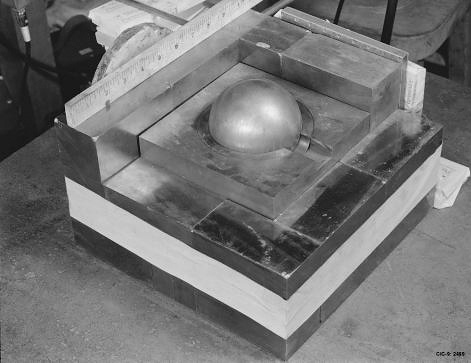
\includegraphics[keepaspectratio, width = 5.0 in]{images/pu_sphere}
    \caption{Plutonium sphere reflected by tungsten-carbide bricks.}
    \label{fig:pu_sphere}
\end{figure}

A second type of accident involves processing operations in which
fissile materials are in solution.  The first domestic processing
accident occured at the Y-12 plant in Oak Ridge, TN.  Y-12 
produces parts from HEU for use in nuclear weapons.  

The accident occured in a portion of the plant used to 
recover HEU from waste material and place it in tanks of favorable
geometry.  These tanks were to be emptied, cleaned, and leak-tested 
with water.  Before the leak-testing began, however, uranium 
solution had leaked from the process stream into the piping
below the storage tanks (and actually into one of the tanks,
as its release valve had been let open).  When the other tanks, full
of water, were emptied, the uranium solution and water accumulated
in a 55 gallon drum.  A nearby worker first noticed dark yellow
fumes followed by a blue flash.  Eight workers received significant
doses, though none died as a result of acute effects.

A rather complete history of criticality accidents in the U.S. and
around the world is contained in the latest edition of
 \textit{A Review of Criticality Accidents} from Los Alamos.  This
document is a really great piece of nuclear history, and students
are highly encouraged to skim through the many accidents covered.

%------------------------------------------------------------------------------
% Computational Aspects
%------------------------------------------------------------------------------

\section*{Computational Aspects}

The intent of this section to provide the reader with an 
overview of criticality safety analysis validation. A brief 
review of regulations and guidance pertinent to criticality safety of 
fissile materials outside reactors is given, with a particular emphasis on 
requirements for ensuring subcritical conditions. The traditional approach to 
bias determination is discussed, and one specific method used in practice
is described and demonstrated in an illustrative example. Subsequently, 
modern S/U-based validation techniques are discussed, and an 
illustrative example is provided and related to the traditional approach.

%------------------------------------------------------------------------------

\subsubsection{Subcritical Limits}

As noted above, ANSI/ANS-8.1 provides guidance 
for avoiding criticality accidents during handling of fissionable material 
outside of reactors \cite{ans8}. The standard provides basic safety principles 
in addition to several limits for simple systems of single isotopes.  
Specifically, the standard defines a \textit{subcritical limit} to be ``the 
limiting value assigned to a controlled parameter that results in a subcritical 
system under specified conditions. The parameter limit allows for 
uncertainties in the calculations and experiemental data used in the derivation 
but not for contingencies.''

These limits are \textit{absolute maxima}, and since they do not include 
contingencies, in practice, adminstrative margins are employed.  A typical 
value, as we'll see below, tends to be 5\% on \keff.

Table \ref{tbl:controlparams} gives several examples of single control 
parameters used in criticality safety analysis.  Note, while ANSI/ANS 8.1 
specifies limits in terms of a single parameter, in some cases, multiple 
parameter limits are also employed.  The standard suggests a few examples, and
cites the technical literature for further guidance. However, while less 
conservative, multiple 
parameter limits require additional adminstrative margins and may be harder to 
use in validation.

\begin{table}[ht]
    \caption{Example single parameters and subcritical limits.}
    \begin{center} 
    \begin{tabular*}{0.90\textwidth}{@{\extracolsep{\fill}} ll } 
      \toprule 
	parameter &  example limit \\
      \midrule
       fissile mass                    &  0.78 kg ${}^{235}$U in UO$_2$NO$_3$ \\
       dimension (width, volume, etc.) &  6.2   L ${}^{235}$U in UO$_2$NO$_3$ \\
       concentration                   &  11.6 g/L${}^{235}$U in UO$_2$NO$_3$ \\
       enrichment                      &  5\%     ${}^{235}$U in UO$_2$       \\
       fissile mass                    &  20.1 kg ${}^{235}$U in UO$_2$ 
                                          (w/ $\rho \leq 18.81$ g/cc) \\
      \bottomrule 
    \end{tabular*} 
    \end{center} 
    \label{tbl:controlparams}
\end{table}

%------------------------------------------------------------------------------


\subsection*{Criticality Safety Analysis Validation}

While the single parameter limits provide useful guidance, two questions 
naturally arise.  First, how does one actually establish these limits?  And 
second, how does one ensure subcriticality in systems that are much more 
complex than, for example, a sphere?  The answer in both cases is by using 
computational methods validated against experiment.

In addition to the single parameter limits, ANSI/ANS-8.1 provides 
requirements for ensuring computational methods used in criticality safety 
analyses are both valid and within the ``area of applicability'' for specific 
applications. The standard defines the area of applicability as ``limiting 
ranges of material compositions, geometric arrangements, neutron energy 
spectra, and other relevant parameters \ldots within which the bias of the 
calculational method is established'' \cite{ans8}.  In other words, an 
\textit{application} is the system of interest, such as a spent fuel canister 
for shipment and disposal. A computational method is \textit{applicable} if 
it is verified against a set of \textit{experiments} that are similar to the 
application with respect to composition, geometry, and so forth.

A \textit{computational bias} is the systematic 
discrepancy between and experimental data and calculated results. Biases 
have associated uncertainties, which quantify the accuracy and 
precision of calculated values and the uncertainty in measured data.

When computational tools are used in criticality safety analyses, the standard
requires that the bias be established.  Qualitatively, the bias must be 
determined via correlating data from critical experiments to computational 
models of the same experiments using the tool to be validated. 
Typically, the measured and 
computed values of \keff are related, but other physical quantities may 
also be used.  The bias is used to normalize a particular code within its 
area of applicability so that its results, after applying the bias, may be 
used to predict criticality within the bias uncertainty.

Another American National Standard, ANSI/ANS-8-17, further explicates 
use of computational tools by defining specific criteria for establishing 
subcriticality \cite{ans8_17}.  Whenever computational methods are 
used in criticality safety analyses, the standard requires that the calculated 
application multiplication factor $k_a$ must be less than or equal to the 
allowable multiplication factor.

The easiest way to think of this is to note that the largest, ``worst case'' 
value for $k_a$ must be below the smallest, least conservative computed 
estimate.  That is to say, the maximum expected application multiplication 
factor (\ie $k_a + \Delta k_a$) must be less than the minimum expected 
computed value (\ie $k_c - \Delta k_c$) for an applicable critical experiment, 
\ie a real, measured system whose \keff is unity, or an average computed 
\keff for several such experiments.  Mathematically, this can be written as
\begin{equation}
 k_a + \Delta k_a \leq k_c - \Delta k_c \, ,
\end{equation}
or
\begin{equation}
 k_a \leq k_c  - \Delta k_a - \Delta k_c \, .
\end{equation}
For added conservatism, the standard further requires that
\begin{equation}
 k_a \leq k_c - \Delta k_a - \Delta k_c - \Delta k_m \, ,
\label{eq:kapp}
\end{equation}
where the standard defines:

\begin{tabular}{rp{10cm}}
 $k_a$           & is the calculated \keff of the 
                   application system for all normal or credible 
                   abnormal conditions; \\
\end{tabular}

\begin{tabular}{rp{10cm}}
 $k_c$           & is the average \keff from the calculation of 
                   the benchmark criticality experiments. 
                   The experiments used 
                   should be neutronically similar to the application
                   system. If the application system has 
                   parameters beyond the area of applicability established 
                   by the benchmark experiments, then the area of 
                   applicability
                   may be extended using trends in the calculated values 
                   of $k_c$ as functions of those parameters; \vspace{12pt} \\
\end{tabular}

\begin{tabular}{rp{10cm}}
 $\Delta k_a$    & is an allowance for 
                 \begin{itemize}
                   \item statistical or convergence uncertainties in 
                         the computed $k_a$;
                   \item material and fabrication tolerances;
                   \item uncertainties due to geometry or material
                         simplifications and approximations;
                 \end{itemize}  \\
\end{tabular}

\begin{tabular}{rp{10cm}}
 $\Delta k_c$    & is a margin for uncertainty in $k_c$ that includes 
                   allowances for
                 \begin{itemize}
                   \item uncertainties in the critical experiments;
                   \item statistical or convergence uncertainties
                         in the computated $k_c$;
                   \item uncertainties due to extrapolation of $k_c$ 
                         outside the experimental data range;
                   \item uncertainties due to geometry or material
                         simplifications and approximations;
                 \end{itemize}
\end{tabular}

\begin{tabular}{rp{12cm}}
 $\Delta k_m$    & is an arbitrary ``administrative'' 
                   margin to ensure the subcriticality 
                   of $k_a$. \\
\end{tabular}

Eq. \ref{eq:kapp} can be rewritten as
\begin{equation}
 k_a + \Delta k_a + \Delta k_m - \beta + \Delta \beta \leq 1 \, ,
\label{eq:kallow}
\end{equation}
where $\beta = k_c - 1$ is the bias and $\Delta \beta = \Delta k_c$ is the 
uncertainty in the bias.  The definition of $\beta$ is based on the fact 
that critical experiments, by their definition, have \keff = 1, and hence 
the bias is just the difference between the computed value and unity.  By 
convention, the bias is defined such that a \textit{ negative} $\beta$ 
indicates an \textit{ underestimated} \keff\!, which is undesirable.

To ensure subcriticality in the application system, an \textit{ upper 
subcritical limit} is defined as
\begin{equation}
 USL = 1 - \Delta k_m + \beta - \Delta \beta \, ,
\label{eq:usl}
\end{equation}
and from Eq. \ref{eq:kallow}, it is apparent that $k_a + \Delta k_a \leq USL$ 
\cite{lichtenwalter1997cbg}.   Thus, the USL is the maximum value an 
application \keff (plus any uncertainties) may have for which the 
application can, with a high degree of confidence, be considered 
subcritical.  The value $1 - USL$  is the mathematical definition of the 
subcritical margin.  In the event the bias $\beta$ is positive, \ie the 
computed value $k_c$ overestimates \keff\!, current practice is to set 
the bias to zero rather than reduce the subcritical margin.

%------------------------------------------------------------------------------

\subsubsection{Traditional Bias Determination}

In the United States, biases and associated uncertainties and USL's have 
often been found through use of \textit{ trending analysis}.  A suite of 
critical experiments is selected for use in a specific safety analysis 
based on the similarity of the experiments to the safety analysis system.  
Traditionally, this similarity is based on physical parameters that include 
the fissile material, hydrogen-to-fissile atom ratio (H/X), average neutron 
energy group causing fission, and energy of average lethargy causing 
fission (EALF), among others \cite{broadhead2004sau}.

While various methods using trending analysis exist for determining the 
biases and USL's, one common approach, denoted USL$_1$ in the 
literature \cite{broadhead2004sau}, is discussed here to provide at least 
some background of current practice. The following description is largely 
adapted from the technical report in which it was first developed 
\cite{lichtenwalter1997cbg}. 

The method computes $k_c(x)$ as a function of a trending parameter $x$ 
using linear regression.  The bias, $\beta(x)$, is just $k_c(x) - 1$.  .  

A lower confidence band $w(x)$ is statistically computed using current 
experiments and uncertainties as well as a specified confidence.  This 
confidence band defines the value below which an additional computed 
\keff value (\ie not included in the analysis) must be for the additional 
system to be considered subcritical with a high degree of confidence.  
Equivalently, for a given value of the trending parameter $x$, $w(x)$ 
represents the value \textit{ above} which the additional computed value $k_c$ 
will be \textit{ if} the system in question is critical---and this consequently 
implies any negative $\beta(x)$ is no worse than $w(x) - 1$.  Hence, if our 
aim is to ensure the actual \keff of a system is subcritical, then its 
computed value should be \textit{ less} than the appropriate confidence band 
value.

To simplify analyses, the limiting width, $W$, of the confidence band is 
used, which (like $w(x)$) takes into account all uncertainties associated 
with the experiments (\eg experimental, stochastic, etc), and consequently, 
is a statistical measure of $\Delta \beta$.  The width $W$ of the 
confidence band is defined
\begin{equation}
 W = \mathrm{max} \Big \{ w(x) | x_{\mathrm{min}},x_{\mathrm{max}} \Big \} \, ,
\label{eq:confwidth}
\end{equation}
where
\begin{equation}
 w(x) = t_{1-\gamma} s_p \Bigg ( 1 + \frac{1}{n} + 
        \frac{(x-\bar{x})^2}{\sum^n_{i=1} (x_i - \bar{x})^2} \Bigg )^{1/2} \, ,
\end{equation}
and $n$ is the number of critical experiments included in the analysis, 
$t_{1-\gamma}$ is the student-t distribution statistic for $1-\gamma$ 
and $n-2$ degrees of freedom ($\gamma$ is the desired confidence level), 
$\bar{x}$ is the mean value of $x$ in the set of experiments, and $s_p$ 
is the pooled standard deviation for the set of calculations.

The pooled standard deviation $s_p$ is defined by
\begin{equation}
 s^2_p = s^2_{k(x)} + s^2_w \, ,
\end{equation}
where $s^2_{k(x)}$ is the mean-square error of the linear regression, 
defined as
\begin{equation}
 s^2_{k(x)} = \frac{1}{n-2} \Bigg ( \sum^n_{i=1} (k_i - \bar{k})^2 - 
              \frac{\Big(\sum^n_{i=1} (x_i-\bar{x})(k_i -\bar{k}) \Big )^2 }
                   {\sum^n_{i=1} (x_i - \bar{x})^2} \Bigg ) \, ,
\end{equation}
and $s^2_w$ is the variance of the data, defined as
\begin{equation}
 s^2_w = \frac{1}{n} \sum^n_{i=1} \sigma^2_i \, ,
\end{equation}
where  $\sigma_i$ is the uncertainty in the $i$th calculated value, 
accounting for method uncertainty (\eg Monte Carlo statistics) and 
estimated uncertainty due to cross-section uncertainty 
(see Section \ref{sec:uncanal}).

The width of the confidence $W$ is chosen to be the \textit{ maximum} value 
of $w$ at the limits of the range of $x$ corresponding to the experiments 
to be conservative, and moreover, it serves to simplify the definition of 
USL.  Current guidance is to define $W$ at the 95\% confidence level, 
\ie choose $\gamma = 0.95$.  See Section \ref{sec:exampletrends} below 
for an illustrative example of the USL$_1$ methodology.

%------------------------------------------------------------------------------

\subsubsection{S/U-Techniques}

Unfortunately, the proper selection of parameters over which to trend, 
and the experiments with which to trend, is largely based on expert 
judgement.  As experiments continue to become more expensive, use of 
computational methods will grow.  Furthermore, new applications will 
continue to extend beyond the areas of applicability of current 
experimental data, and consequently, methods to extend beyond these 
areas are needed.

For the past several years, ORNL has worked with the support of the 
NRC and the Department of Energy's (DOE) Nuclear Criticality Safety 
Program to develop ``a rigorous physics-based approach for the 
determination of system similarity'' for determining areas of 
applicability \cite{broadhead2004sau}.  Additionally, their efforts 
aimed to develop the methodology and computational tools needed for 
``determination of biases and uncertainties due to experimental 
descriptions, computational methods, and nuclear data.''

As an alternative to traditional trending analysis, work was done to 
develop S/U-based, easily-quantifiable parameters to measure the 
similarity of systems.  It is beyond our scope to describe the 
methods in detail.  Interested readers should see the exercises
of Lecture \ref{lec:the_adjoint_and_perturbation_theory} for some
basic theory needed to derive the results, and Ref. 
\cite{broadhead2004sau} for greater detail.

Skipping the theory, what we end up with is the sensitivity
of \keff to the various underlying nuclear data, 
\begin{equation}
 S_{k,\sigma_x} = \frac{\sigma_x}{k}\frac{\partial k}{\partial \sigma_x} 
 \label{eq:keffsens}
\end{equation}
where $x$ denotes some reaction of interest.  We express the sensitivity 
of \keff to all nuclides in a system as the vector $\mathbf{S}_k$,
which can implicitly represent dependence on multigroup data.

Sensitivity vectors can be used to compare both the qualitative and 
quantitative similarity between two systems with respect to single or 
several nuclide-reactions. Let the entire set of group-wise, nuclide-reaction 
cross-sections be denoted 
$\bm{\sigma} \equiv \sigma_i, \; \; n = 1,\;2,\ldots,N$, where $N$ is the 
total number of nuclide-reactions multiplied by the number of energy 
groups.  The $N\times N$ correlation (\ie relative covariance) matrix 
of $\bm{\sigma}$ is defined
\begin{equation}
\mathbf{C_{\sigma \sigma}} \equiv \Bigg[\frac{\mathrm{COV}(\sigma_i,\sigma_j)}
                                             {\sigma_i \sigma_j} \Bigg ] \, ,
\end{equation}
where $i$ and $j$ range from 1 to $N$, and 
\begin{equation}
\mathrm{COV} = \langle (\sigma_i - \bar{\sigma_i})(\sigma_j - 
               \bar{\sigma_j}) \rangle 
             = \langle \delta \sigma_i \delta \sigma_j \rangle \, ,
\end{equation}
where $\bar{\sigma_i}$ represents the expected value of the data $\sigma_i$.  

Because the components of \cov represent relative uncertainties, and because 
from above, we know the \keff sensitivity represents the relative change in 
\keff due to relative changes in some nuclide-reaction data, the relative 
uncertainty in \keff is therefore
\begin{equation}
\frac{\delta k}{k} = \sqrt{ \mathbf{S}_k \mathbf{C_{\sigma \sigma}} 
                     \mathbf{S}_k^T } \, ,
\end{equation}
where $T$ denotes the matrix transpose.  If several systems are of interest, 
then an $N \times I$  matrix of sensitivity vectors $\mathbf{\bar{S}}_k$ can 
be defined, where $I$ is the number of systems.  By folding 
$\mathbf{\bar{S}}_k$ with \cov, one obtains
\begin{equation}
 \mathbf{C}_{kk} =  \mathbf{\bar{S}}_k \mathbf{C_{\sigma \sigma}} 
                    \mathbf{\bar{S}}_k^T  \, ,
\label{eq:kunc}
\end{equation}
an $I\times I$ matrix consisting of each system's relative variance in 
\keff (\ie $(\Delta k/k)^2$) due to data uncertainties (the diagonal terms, 
$\alpha_{ii}$) and the relative covariances in \keff between systems 
(the off-diagonal terms, $\alpha_{ij}$).  These off-diagonal terms 
represent ``shared variance'' or ``shared uncertainty'' between systems.  

The correlation coefficient between system $i$ and $j$ is defined
\begin{equation}
 c_{k} =  \frac{\alpha^2_{ij}}{\alpha_i \alpha_j}  \, ,
\label{eq:ck}
\end{equation}
which, as is expected, takes on values between -1 
(completely anti-correlated) and 1 (completely correlated). 
A value $c_k = 0$ indicates no correlation between systems.  

The correlation of two systems is greatest if they share basic 
characteristics, \eg fuel type, moderator, other materials.  Two 
water-moderated thermal UO$_2$ systems would be expected to have 
a higher degree of correlation than would such a thermal system 
and a molten salt fast reactor.  Use of $c_k$ as a trending 
parameter in the USL$_1$ method is illustrated below.

%------------------------------------------------------------------------------

\subsubsection{Example Analyses}

To illustrate the USL$_1$ method using both traditional parameters 
and $c_k$, 25 thermal LEU systems were chosen for example analyses.  
Two additional systems were selected as ``applications'' for which 
the $\beta$, $\Delta \beta$, and the USL are determined\footnote{The 
minimum recommended number of experiments for trending with the 
USL$_1$ method is 25; here, just the minimum was used for these example 
cases.}. The experiments range from 2.35\% to 5\% enrichement, and have 
EALF values ranging from 0.017 to 2.24 eV.  %These parameters, along 
%with $c_k$ with respect to the two applications (LCT-079-002 and 
%LCT-050-001), are provided in Table \ref{tbl:exampletrend}. 
All experiments 
are included in the International Handbook of Evaluated Criticality Benchmark 
Experiments \cite{ihecsbe} and are low enriched uranium, thermal assemblies.
The LCT-079 and LCT-050 are experiments
of use to burnup credit, a topic discussed below; however, their use here
is purely for example.  

Figures \ref{fig:trend_ealf}-\ref{fig:trend_ck2} show the trending analysis 
for using EALF, enrichment, and $c_k$.  For both EALF and enrichment, only 
one analysis was needed for the applications since neither parameter depends 
on the application.  However, separate cases were run using $c_k$ values 
specific to the given application.  The experiments are the black dots, 
and the applications are red shapes.  For all cases, the uncertainty is 
computed using Eq. \ref{eq:kunc}, where the uncertainty for the system is 
its associated diagonal element of $\mathbf{C}_{kk}$, \ie the uncertainty 
in cross-sections propagated to \keff via use of sensitivity profiles.  
This is in line with previous analyses \cite{broadhead2004sau}.  Note, for 
the USL, an administrative margin of $\Delta k_m = 0.05$ was used.

% \begin{table}[hp]
%  \caption{Experiment and test application parameters.  Note (a) and (b) refer to the LCT-079 and LCT-050 experiments.}
%  \begin{center} 
%  \begin{tabular*}{0.95\textwidth}{@{\extracolsep{\fill}} ccccccc } 
%   \toprule 
%          Id.       &  \keff   & $\sigma_k$&  EALF (eV)&  Enrich.(\%) & $c_k$ (a) & $c_k$ (b)    \\ 
%    \midrule
%   LCT-010-005  &  0.9951  &  0.0050  &  3.89E-01  &  4.306  &  0.861  &  0.890  \\
%   LCT-010-016  &  0.9936  &  0.0058  &  2.92E-01  &  4.306  &  0.977  &  0.982  \\
%   LCT-010-017  &  0.9937  &  0.0058  &  2.86E-01  &  4.306  &  0.979  &  0.983  \\
%   LCT-010-018  &  0.9924  &  0.0058  &  2.81E-01  &  4.306  &  0.980  &  0.985  \\
%   LCT-010-019  &  0.9917  &  0.0058  &  2.74E-01  &  4.306  &  0.980  &  0.986  \\
%   LCT-017-003  &  0.9927  &  0.0055  &  9.57E-02  &  2.350  &  0.899  &  0.924  \\
%   LCT-017-004  &  0.9919  &  0.0052  &  2.17E-01  &  2.350  &  0.827  &  0.850  \\
%   LCT-017-005  &  0.9945  &  0.0053  &  1.89E-01  &  2.350  &  0.851  &  0.876  \\
%   LCT-017-006  &  0.9939  &  0.0054  &  1.78E-01  &  2.350  &  0.862  &  0.888  \\
%   LCT-017-007  &  0.9937  &  0.0053  &  1.69E-01  &  2.350  &  0.858  &  0.884  \\
%   LCT-042-001  &  0.9906  &  0.0054  &  1.73E-01  &  2.350  &  0.797  &  0.764  \\
%   LCT-042-002  &  0.9909  &  0.0055  &  1.79E-01  &  2.350  &  0.801  &  0.767  \\
%   LCT-042-003  &  0.9897  &  0.0054  &  1.86E-01  &  2.350  &  0.779  &  0.747  \\
%   LCT-042-004  &  0.9918  &  0.0054  &  1.84E-01  &  2.350  &  0.768  &  0.736  \\
%   LCT-042-005  &  0.9921  &  0.0057  &  1.81E-01  &  2.350  &  0.891  &  0.862  \\
%   LCT-049-001  &  0.9904  &  0.0057  &  2.02E+00  &  5.000  &  0.889  &  0.860  \\
%   LCT-049-002  &  0.9914  &  0.0057  &  2.03E+00  &  5.000  &  0.895  &  0.867  \\
%   LCT-049-003  &  0.9913  &  0.0055  &  2.15E+00  &  5.000  &  0.877  &  0.849  \\
%   LCT-049-004  &  0.9906  &  0.0058  &  2.24E+00  &  5.000  &  0.932  &  0.910  \\
%   LCT-049-005  &  0.9915  &  0.0059  &  1.14E+00  &  5.000  &  0.934  &  0.911  \\
%   LCT-049-006  &  0.9900  &  0.0055  &  1.15E+00  &  5.000  &  0.889  &  0.894  \\
%   LCT-049-007  &  0.9904  &  0.0053  &  1.11E+00  &  5.000  &  0.873  &  0.878  \\
%   LCT-049-008  &  0.9906  &  0.0053  &  1.19E+00  &  5.000  &  0.862  &  0.867  \\
%   LCT-049-009  &  0.9912  &  0.0053  &  7.39E-01  &  5.000  &  0.869  &  0.873  \\
%   LCT-049-010  &  0.9904  &  0.0053  &  7.47E-01  &  5.000  &  0.869  &  0.874  \\
%   \midrule
%   LCT-079-002  &  0.9897  &  0.0069  &  2.03E+00  &  4.310  &  1.000  &  na     \\
%   LCT-050-001  &  0.9906  &  0.0067  &  1.99E-01  &  4.738  &  na     &  1.000  \\
%   \bottomrule 
%  \end{tabular*} 
%  \end{center} 
%  \label{tbl:exampletrend}  
% \end{table}

\begin{figure}[htp] 
    \centering
    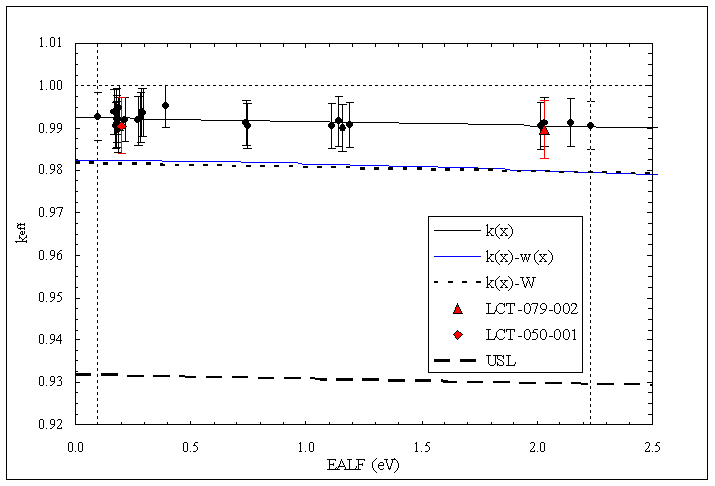
\includegraphics[keepaspectratio, width = 5 in]{images/trend_ealf}
    \caption{Example trending analysis using EALF.}
    \label{fig:trend_ealf}
\end{figure}


\begin{figure}[htp] 
    \centering
    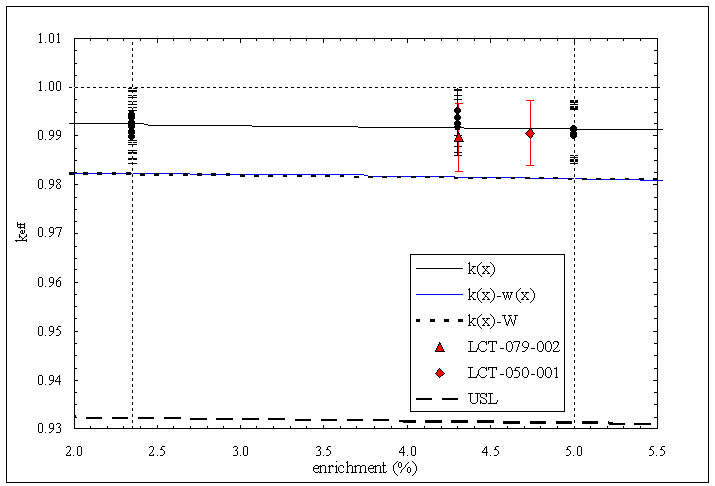
\includegraphics[keepaspectratio, width = 5 in]{images/trend_enrich}
    \caption{Example trending analysis using enrichment.}
    \label{fig:trend_enrich}
\end{figure}


\begin{figure}[htp] 
    \centering
    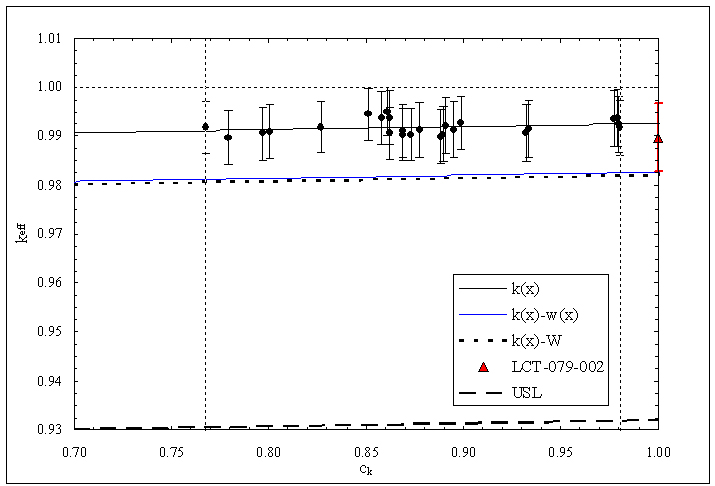
\includegraphics[keepaspectratio, width = 5 in]{images/trend_ck1}
    \caption{Example trending analysis using $c_k$ (for LCT-079-002).}
    \label{fig:trend_ck1}
\end{figure}


\begin{figure}[htp] 
    \centering
    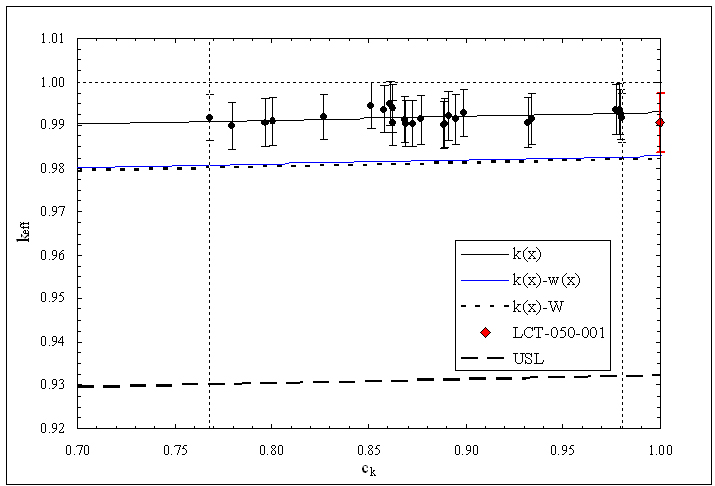
\includegraphics[keepaspectratio, width = 5 in]{images/trend_ck2}
    \caption{Example trending analysis using $c_k$ (for LCT-050-001).}
    \label{fig:trend_ck2}
\end{figure}

From the trends, the bias $k(x)-1$ (where $x$ is the parameter value 
for the application) and associated bias uncertainty (\ie $W$ from 
Eq. \ref{eq:confwidth}) can be computed in addition to the USL.  
Since the ``applications'' are known critical experiments, it is useful 
to compare the observed bias (\ie $k_{\mathrm{calc}} -1$) to the bias 
as predicted via trending.  Table \ref{tbl:trendbias} provides the 
observed and predicted biases (with uncertainty) and the USL for both 
applications.  For each application, all three methods yield very similar 
USL's, and all the biases are slightly underpredicted but well within 
one standard deviation of the observed biases.  

With such a large $\Delta k_m$, it is easy to wonder why we care 
about $\Delta \beta$. However, if we interpret subtracting $\Delta k_m$ 
from \keff as simply shifting the definition of critical, then it 
becomes clearer that $\Delta \beta$ is still important.

{\tiny
\begin{table}[hp]
 \caption{Observed and predicted biases ($\beta_{\mathrm{ob}}$ and 
         $\beta$), $\Delta \beta$, all in percent, and USL using 
         each trending technique.}
 \begin{center} 
 \begin{tabular*}{0.98\textwidth}{@{\extracolsep{\fill}} c|cccc|cccc } 
  \toprule
              & \multicolumn{4}{c}{LCT-079-002}          & \multicolumn{4}{c}{LCT-050-001} \\
   \midrule 
             & $\beta_{\mathrm{ob}}$ & $\beta$ & $\Delta \beta$  & USL & $\beta_{\mathrm{ob}}$& $\beta$  & $\Delta \beta$ & USL \\ 
   \midrule
       EALF  &  -1.08  &  -0.95  &  1.08  &  0.9298  &  -0.94  &  -0.77  &  1.08  &  0.9316 \\
    Enrich.  &  -1.08  &  -0.84  &  1.02  &  0.9314  &  -0.94  &  -0.85  &  1.02  &  0.9313 \\
      $c_k$  &  -1.08  &  -0.74  &  1.16  &  0.9306  &  -0.94  &  -0.71  &  1.07  &  0.9322 \\
  \bottomrule 
 \end{tabular*} 
 \end{center} 
 \label{tbl:trendbias}  
\end{table} 
}

\section*{Case Study: Burnup Credit}

\subsubsection*{Overview and Motivation}

The transportation and storage of used nuclear fuel is an integral component of any
nuclear fuel cycle. During handling of used nuclear fuel, strict attention must be paid
to criticality safety. The chief concern of criticality safety is to ensure the effective
multiplication factor \keff of the system in question is below unity at all times, i.e. to
ensure subcriticality.
For the case of used nuclear fuel, several factors affect the subcritical margin, i.e.
by how much a system is subcritical. Typical, unirradiated light water reactor (LWR)
fuel consists of uranium-oxide (UO2 ) enriched to 3-5\% ${}^{235}$U. During its time in the
reactor, nuclear fuel undergoes significant compositional changes, a process referred
to as burnup. Most importantly, the fissile isotope 235 U is depleted, generating various
fission products (FP's), many of which are parasitic neutron absorbers. Simultaneously,
${}^{235}$U breeds ${}^{239}$Pu which also undergoes fission and produces FP's. The net
effect of these compositional changes is to decrease the \keff of the fuel with increased
burnup. Accounting for this decrease in \keff (or equivalently, a decrease in reactivity)
in subcritical margins is often referred to as \textit{burnup credit}.

Historically, the so-called \textit{fresh fuel assumption} was used as a conservative bound
in criticality safety analysis of used nuclear fuel [1]. More recently, the Nuclear
Regulatory Commission (NRC) offered guidance for crediting the major (fissile) actinides
in such analyses in its Interim Staff Guidance - 8, revision 2 (ISG-8R2) report [2]. However,
even this results in a very conservative estimate of the subcritical margin of used
nuclear fuel.

Changes in the major actinides account for about 66-75\% of the net reduction
in reactivity; FP's account for the remainder, the percentages depending on burnup.
The FP's relevant to burnup credit, roughly in order of importance, include SM.
 
Why do we care?  Naturally, assuming a canister of some number of burned assemblies 
contains only fresh fuel is quite conservative.  Figure \ref{fig:loading_curve} shows 
loading curves for a generic used fuel canister with 32 WH 17x17 assemblies of varying 
initial enrichments and burnups.  Configurations below a given line do not meet subcritical 
limits under the given assumptions.  The reference case assumes fresh fuel, and each 
subsequence curve relaxes the assumptions.  

Considering that much of the current U.S. inventory of used fuel lies below the reference 
curve, a 32-assembly canister could not be widely used (and instead, canisters such as
the 21-assembly Transportation, Aging, and Disposal (TAD) canister intended for ultimate
disposition in Yucca Mountain would be required).  The cost of producing, loading, shipping, 
and disposing canisters is not negligible, and a study by Parks and Wagner suggest that
crediting the FP's in criticality safety analysis, thus allowing the high capacity
canisters, would potentially save upwards of \$200 million dollars in total disposal
costs \cite{parks2004csp}. 

\begin{figure}[ht] 
    \centering
    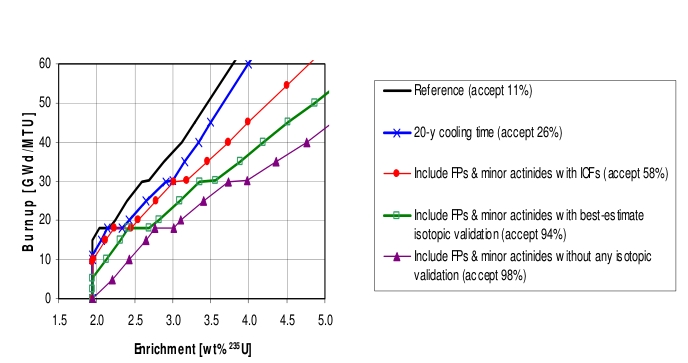
\includegraphics[keepaspectratio, width = 5.0 in]{images/loading_curve}
    \caption{Effect of calculational assumptions on loading curves for the GBC-32 and WH 17x17 assemblies.}
    \label{fig:loading_curve}
\end{figure}

\subsubsection*{Current Research}

To take into account the reduction in reactivity due to fission products,
called \textit{full burnup credit}, requires adequate knowledge of the 
isotopic content of the spent fuel (via validated depletion methods), and, 
our focus here, \textit{methods} to determine criticality and 
\textit{experiments} to validate those methods.

Current work has expanded on the S/U-based techniques
outlined above to develop methods for determinining biases of 
individual nuclides. While the details are beyond our scope, we give 
a brief description and several references for interested readers.

The basis of the work is the generalized linear least-square method (GLLSM).
GLLSM takes as input a set of nuclear data and covariances, the sensitivities 
of experiment models to nuclear data, the model \keff and uncertainty,
the experiment \keff and uncertainty (and any experiment correlation), 
and \textit{adjusts the nuclear data}
so that the the experiment and model \keff match.  It does so in a way that
minimizes the variation of all parameters (data and \keff) in terms of the
standard deviations of those parameters.  In other words, for all parameters
$p$, the method forces the experiment and model \keff to match while 
minimizing $\sum_i (\Delta p_i / \sigma_{p_i})^2$.  The adjustments can be 
propogated to an application's \keff via its model sensitivities, and the 
resulting difference is the bias.

To find biases of individual nuclides, the GLLSM method can be applied to 
so-called ``replacement experiments''.  These experiments consists of a single
reference case, and one or more cases that introduce some small perturbation
to the system, such as small foils of a fission product between fuel pellets 
\cite{buccx} or small concentrations of a fission product in a bulk
moderator \cite{french}.  GLLSM can then be applied to the reactivity 
difference between a reference-perturbation pair of models and experiements 
(rather than on the eigenvalue), since the sensitivities of the 
reactivity difference should be small for all but the perturbation 
material.  Consequently, the corresponding adjustment to the data should 
primarily be due to the test material, and as above, the adjustment can 
be propogated to the application to define a nuclide-specific bias.

\subsubsection{Limitations}

Two significant limitations apply to the methods under development.  First,
the methods require that relevant experiments are available.  However,
only a handful of experiments have been performed relevant to burnup credit,
and of those, the difference between reference and perturbation cases may 
be too high to extract partial biases.  Moreover, little data is available
for the correlation between experiments.  For the the reactivity difference
method described above, the resulting biases are extremely sensitive to 
the correlation between experiments. This suggests that future 
experiments should be designed with the various S/U methods as guidance.

A second, perhaps more significant issue is the general lack of reliable
nuclear covariance data.  Only for the most important isotopes does credible
data exist (such as uranium isotopes).  For isotopes of generally less
importance (like many fission products), little if any covariance data
exists.  Until reliable covariance data exists, the methods described
above are of limited value.
 
\section{Further Reading}

Much of the content in this lecture was inspired by Knief's 
\textit{Nuclear Criticality Safety: Theory and Practice} \cite{knief}.  Of
course, in one lecture, all that material cannot be covered, and the student
is directed to that book for more info most of the topics addressed here.
A more succinct overview of some of the topics is given by 
Peavey
in the \textit{Handbook of Nuclear Engineering} \cite{handbook}.  

For an overview of the application of sensitivity and uncertainty analysis
to criticality safety, see Broadhead et. al \cite{broadhead2004sau}, and
for the latest work on adjustment techniques applicable to full burnup
credit, see Rearden et al. \cite{reardenNT}.
% 
% \part{Deterministic Transport} 
% 
% \chapter{The Transport Equation}

In this lecture, we introduce general \textit{transport equations} and finish by developing the form used in neutron transport theory.  In the lectures to follow, we shall describe other aspects of the neutron transport equation and methods by which it can be solved both analytically and numerically.

\section*{Transport Theory}

Transport theory aims to describe mathematically the movement (i.e. ``transport'') of particles as they traverse a medium.  For example, we might describe the transport of high energy gammas through a lead shield, or the movement of neutrons through uranium dioxide pellets.  We might also describe the movement of particles in a dense gas as they navigate through a medium consisting of the gas itself.

In all cases, transport theory describes such processes in an \textit{average} sense.  For instance, we do not compute the individual trajectories of neutrons in a reactor via transport theory.  That, instead, would require molecular dynamics, in which Newton's equation of force is solved for the many-bodied problem of all neutrons in the vicinity of interest (an essentially impossible problem), or perhaps the Monte Carlo methods described in previous lectures, where a sample of individual particles are tracked to approximate ensemble averages (a difficult, but as we've seen, tractable problem).  Hence, the quantities we shall compute using the equations of transport theory should be recognized as expected and not exact values.

\section*{Fundamental Quantities}

We begin by defining several fundamental quantities.  It should be noted that the forms introduced at first are likely different from what you might have seen in a previous reactor physics course.  The purpose here is two-fold.  First, we wish to introduce the quantities and eventually the equations in a general way to make clear that transport theory is not restricted to the neutron transport equation.  Second, for those who might be familiar with e.g. the Boltzmann equation of gas dynamics (and not neutron transport), the notation will be familiar and lead smoothly into our more familiar form.

We first define the \textit{phase space density function}, the knowledge which we can use to compute essentially all quantities of interest:
\begin{center}
  \begin{tabular}{cp{7.0cm}}
    $n(\mathbf{r},\mathbf{v},t)d^3r d^3v \equiv $ &
    expected number of particles in  $d^3r$  about  $\mathbf{r}$  with velocity  $dv$ about  $\mathbf{v}$ at time $t$.  
  \end{tabular}
\end{center}
It is often most convenient to break the velocity into its scalar (speed) and vector (direction) components.  The scalar component is recast in the energy variable via $E = mv^2/2$, and the direction vector is defined $\mathbf{\Omega}=\mathbf{v}/|\mathbf{v}|$.  The phase space density can then be rewritten as
\begin{center}
  \begin{tabular}{cp{7.0cm}}
    $n(\mathbf{r},\mathbf{\Omega},E,t)d^3r d\Omega dE \equiv $ &
    expected number of particles in  $d^3r$  about  $\mathbf{r}$  going in the directions $d\Omega$ about $\mathbf{\Omega}$ with energy  $dE$ about  $E$ at time $t$.  
  \end{tabular}
\end{center}
In this form, $n(\mathbf{r},\mathbf{\Omega},E,t)$ is often referred to as the angular density.

\begin{wrapfigure}{r}{0.5\textwidth}
    \begin{center}
    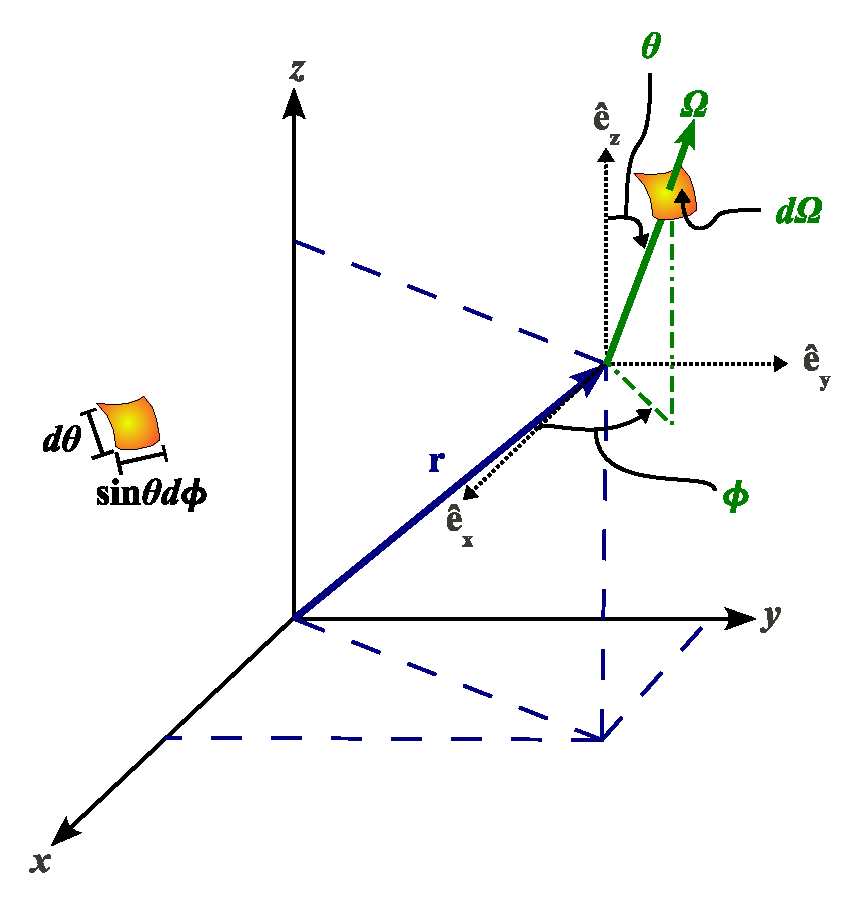
\includegraphics[keepaspectratio, width = 2.7 in]{images/phase_space}
    \end{center}
    \caption{Schematic of Phase Space.}
    \label{fig:phase_space}
\end{wrapfigure}

We can relate the phase space densities in terms of $\mathbf{v}$ and $(E,\mathbf{\Omega})$ via the relations
\begin{equation}
 \begin{split}
  n(\mathbf{r},E,\mathbf{\Omega},t) &= (v/m) n(\mathbf{r},\mathbf{v},t) \\
  n(\mathbf{r},E,\mathbf{\Omega},t) &= (1/mv) n(\mathbf{r},v,\mathbf{\Omega},t) \\
  n(\mathbf{r},v,\mathbf{\Omega},t) &= v^2 n(\mathbf{r},\mathbf{v},t) \, ,
 \end{split}
 \label{eq:densityrelations}
\end{equation}
proofs of which are left as exercises.

Figure \ref{fig:phase_space} depicts a schematic of the phase space used in terms of the position $\mathbf{r}$ and direction $\mathbf{\Omega}$.  The position vector is further broken down into the polar angle $\theta$ and azimuthal angle $\phi$.  The differential solid angle element $d\Omega$ is also shown, and can be expressed in terms of $\theta$ and $\phi$ via
\begin{equation*}
 d\Omega = \sin{\theta} d\theta d\phi \, .
\end{equation*}  
One might envision such solid angle elements as the small bumps on basketballs.  

A quantity closely related to the phase space density (or current density) is the \textit{angular current density}:
\begin{center}
  \begin{tabular}{cp{5.0cm}}
    $\mathbf{j}(\mathbf{r},\mathbf{v},t)\cdot d\mathbf{S} d^3v = \mathbf{v} n(\mathbf{r},\mathbf{v},t) \cdot d\mathbf{S} d^3v \equiv $ &
    expected number of particles that cross an area $dS$ per second with velocity $d^3v$ about $\mathbf{v}$ at time $t$.
  \end{tabular}
\end{center}

We can also define \textit{partial currents} with respect to a particular surface $S$ defined by an outward normal vector $\mathbf{\hat{e}}_s$:

\begin{center}
  \begin{tabular}{cp{5.0cm}}
    $J_{\pm}(\mathbf{r},t) = \pm \int_{\pm} d^3v  \mathbf{\hat{e}}_s \cdot \mathbf{j} (\mathbf{r},\mathbf{v},t) \equiv $ &
   the rate at which particles flow through $S$ in the outward (+) or inward (-) direction.
  \end{tabular}
\end{center}

The \textit{current density} $\mathbf{J}(\mathbf{r},t)$ is defined by integrating the angular current density over all velocities.  Then for our surface $S$, the net rate of particles passing outward through $S$ is just $\mathbf{J}(\mathbf{r},t) \cdot \mathbf{\hat{e}}_s$.  From our definition of partial currents, the net current passing outward must also be $J_+ - J_-$, yielding the useful identity
\begin{equation}
 \mathbf{J}(\mathbf{r},t) \cdot \mathbf{\hat{e}}_s = J_{+}(\mathbf{r},t) - J_{-}(\mathbf{r},t) \, .
 \label{eq:net2partial}
\end{equation}

%A point of caution: it should be noted that $n$ and $\mathbf{j}$ must have the same units but represent wholly different things since $n$ is a scalar quantity while $\mathbf{j}$ is a vector quantity.  This will be true also of $\mathbf{J}$ and the scalar flux $\phi$, which will be introduced

Of particular interest to us in the next section will be reaction rates, which can most easily be described using the \textit{angular flux}
\begin{center}
  \begin{tabular}{cp{2.0cm}}
    $ \psi (\mathbf{r},\mathbf{\Omega},E,t) = v n(\mathbf{r},\mathbf{\Omega},E,t) \equiv $ &
    angular flux
  \end{tabular}
\end{center}
and \textit{scalar flux}
\begin{center}
  \begin{tabular}{cp{2.0cm}}
    $ \phi (\mathbf{r},E,t) = \int_{4\pi} d\Omega \psi (\mathbf{r},\mathbf{\Omega},E,t)  \equiv $ &
    scalar flux.
  \end{tabular}
\end{center}

\section*{A General Transport Equation}

Consider an arbitrary volume $V$ with a surface $S$.  Our goal is to represent the time rate of change of the particle density $n(\mathbf{r},\mathbf{v},t)$ within the volume.  Neglecting external forces, the only factors affecting the density are collisions within the volume that change a particle's velocity, the streaming of particles into and out of the surface, and any internal source of particles.  This simple balance can be expressed mathematically as
\begin{equation}
\begin{split}
 \overbrace{ \frac{\partial}{\partial t} \Bigg ( \int_V d^3 r n(\mathbf{r},\mathbf{v},t) \Bigg ) }^{\text{total rate of change of }n\text{ in } V} 
      &=  - \overbrace{\int_S dS \mathbf{\hat{e}}_S \cdot \mathbf{j}(\mathbf{r},\mathbf{v},t) }^{\text{streaming rate}}
       + \overbrace{ \int_V d^3 r \Big( \frac{\partial n}{\partial t} \Big )_{\mathrm{coll}} }^{\text{collision rate}} \\
      &+ \underbrace{ \int_V d^3 r s(\mathbf{r},\mathbf{v},t) }_{\text{source emission rate}}  \, ,
\end{split}
\label{eq:balance}
\end{equation}
where $s$ represents a source inside the volume and $(\partial n/\partial t)_{\mathrm{coll}}$ is the time rate of change due to collisions, specific forms of which are application-dependent and will be discussed below.  Note the minus sign on the surface integral, i.e. the streaming term.  Since the integral describes the net rate of neutrons going \textit{out} of the surface, we negate it so that a positive net rate directed inward is a positive contribution to the total time rate of change of $n$ in $V$.

Eq. \ref{eq:balance} gives us a simple relation in terms of both volume and surface integrals.  Our life is always easiest if we have the same integration on both sides.  By the divergence (or Gauss') theorem, we can rewrite the streaming term
\begin{equation}
 \int_S dS \mathbf{\hat{e}}_S \cdot \mathbf{j}(\mathbf{r},\mathbf{v},t) = \int_V d^3r \nabla \cdot \mathbf{j}(\mathbf{r},\mathbf{v},t) \, .
\end{equation}
Since $\nabla$ acts on $\mathbf{r}$ and not $\mathbf{v}$, we note $ \nabla \cdot \mathbf{j} = \nabla \cdot (\mathbf{v} n) =  \mathbf{v} \cdot \nabla n + \overbrace{ n \nabla \cdot \mathbf{v}}^{\to 0} = \mathbf{v} \cdot \nabla n$.  Hence, the streaming term becomes
\begin{equation}
 \int_V d^3r \nabla \cdot \mathbf{j}(\mathbf{r},\mathbf{v},t) = \int_V d^3r \mathbf{v} \cdot \nabla n(\mathbf{r},\mathbf{v},t) \, .
\end{equation}

For a constant volume, $(\partial/\partial t) \int_V d^3 r n = \int_V d^3 (\partial n/\partial t)$, and so our balance equation can be rewritten as
\begin{equation}
\begin{split}
 \overbrace{  \Bigg ( \int_V d^3 r \frac{\partial}{\partial t}n(\mathbf{r},\mathbf{v},t) \Bigg ) }^{\text{total rate of change of }n\text{ in } V} 
      &=  - \overbrace{\int_V d^3r \mathbf{v} \cdot \nabla n(\mathbf{r},\mathbf{v},t)}^{\text{streaming rate}}
       + \overbrace{ \int_V d^3 r \Big( \frac{\partial n}{\partial t} \Big )_{\mathrm{coll}} }^{\text{collision rate}} \\
      &+ \underbrace{ \int_V d^3 r s(\mathbf{r},\mathbf{v},t) }_{\text{source emission rate}}  \, .
\end{split}
\label{eq:balance2}
\end{equation}
For an arbitrary volume $V$, the integrands of Eq. \ref{eq:balance2} must vanish, yielding a general transport equation:
\begin{equation}
  \frac{\partial}{\partial t}n(\mathbf{r},\mathbf{v},t) = -\mathbf{v} \cdot \nabla n(\mathbf{r},\mathbf{v},t) + \Big( \frac{\partial n}{\partial t} \Big )_{\mathrm{coll}} +  s(\mathbf{r},\mathbf{v},t) \, .
\end{equation}

\section*{Even More Generality}
We can skip the differential volume formulation by considering the material derivative of $n$ (using Cartesian coordinates):
\begin{equation}
 \begin{split}
 \frac{Dn}{Dt} &\equiv \frac{ \partial n}{\partial t} 
 + \frac{\partial x}{\partial t}\frac{\partial n}{\partial x} + \frac{\partial y}{\partial t}\frac{\partial n}{\partial y} + \frac{\partial z}{\partial t}\frac{\partial n}{\partial z} +  \frac{\partial v_x}{\partial t}\frac{\partial n}{\partial v_x} +  \frac{\partial v_y}{\partial t}\frac{\partial n}{\partial v_y} +  \frac{\partial v_z}{\partial t}\frac{\partial n}{\partial v_z} \\
               &= \frac{ \partial n}{\partial t} + \mathbf{v}\cdot \nabla n + \mathbf{a} \cdot \nabla_{\mathbf{v}} n \\
               &= \frac{ \partial n}{\partial t} + \mathbf{v}\cdot \nabla n + \frac{\mathbf{F}}{m} \cdot \nabla_{\mathbf{v}} n \, ,\\
 \end{split}
\end{equation}
where $\nabla_{\mathbf{v}}$ is the gradient operator with respect to velocity components (rather than spatial coordinates).  The material derivative is the total time rate of change, accounting for convective (streaming) effects as well as the influence of an external force $\mathbf{F}$, a factor we did not account for above.  

This total rate of change must be balanced by sources and sinks, which are the collision and internal source terms.  Hence, an even more general transport equation can be written
\begin{equation}
  \frac{\partial n}{\partial t} + \mathbf{v} \cdot \nabla n + \frac{\mathbf{F}}{m} \cdot \nabla_{\mathbf{v}} n =   \Big( \frac{\partial n}{\partial t} \Big )_{\mathrm{coll}} +  s \, .
 \label{eq:generalte}
\end{equation}

\section*{Neutron Transport}

To arrive at the neutron transport equation, we bring back the macroscopic cross-sections studied in Lecture \ref{lec:macro}.  Using our definition for the scalar flux, the volumetric collision rate at a particular point in phase space and time is simply
\begin{equation}
 R_{\text{coll}}(\mathbf{r},\mathbf{\Omega},E,t) = \psi(\mathbf{r},\mathbf{\Omega},E,t) \Sigma_t(\mathbf{r},E) \, .
\end{equation}
However, we know that neutrons at one energy and angle can scatter into another energy and angle, and so in general, the rate at which neutrons at any angle and energy are scattered into a particular energy and angle is
\begin{equation}
 R_{\text{in-scatter}}(\mathbf{r},\mathbf{\Omega},E,t) = \int^{\infty}_{0} dE' \int_{4\pi} d\Omega' \Sigma_s(\mathbf{r},\mathbf{\Omega}\cdot\mathbf{\Omega}',E'\to E)\psi(\mathbf{r},\mathbf{\Omega'},E',t) \, .
\end{equation}
The time rate of change due to collisions is thus
\begin{equation}
\begin{split}
 \Big( \frac{\partial n}{\partial t} \Big )_{\mathrm{coll}} &= -\psi(\mathbf{r},\mathbf{\Omega},E,t) \Sigma_t(\mathbf{r},E)  \\
  &+ \int^{\infty}_{0} dE' \int_{4\pi} d\Omega' \Sigma_s(\mathbf{r},\mathbf{\Omega}'\to \mathbf{\Omega},E'\to E)\psi(\mathbf{r},\mathbf{\Omega'},E',t) \, .
\end{split}
\end{equation}
Substituting this into the general transport equation, using $\psi = vn$, and neglecting any external forces, we find the neutron transport equation:
\begin{equation}
  \begin{split}
     \frac{1}{v}\frac{\partial \psi}{\partial t} &+ \hat{\Omega} \cdot \nabla \psi + \Sigma_t \psi(\mathbf{r},\mathbf{\Omega},E,t) = \\
           &+ \int^{\infty}_{0} dE' \int_{4\pi} d\Omega' \Sigma_s(\mathbf{r},\mathbf{\Omega}\cdot\mathbf{\Omega}',E'\to E)\psi(\mathbf{r},\mathbf{\Omega'},E',t) +s \, .
  \end{split}
  \label{eq:neutrontransport}
\end{equation}
Note, the source term $s$ has been used to represent internal sources but could also account for other sources such as fission (though the specific form is, of course, hidden).

\section*{Assumptions for the Neutron Transport Equation}
In writing down Eq. \ref{eq:neutrontransport} as we have, a number of assumptions have been made explicitly or implicitly.  These include:
\begin{enumerate}
   \item The neutron density is large so that it makes sense to be computing for mean values (which is all transport equations can provide)
   \item The neutrons are point particles, meaning that wave effects are insignificant
   \item Collisions are well-defined, two-body interactions that occur instantaneously (delayed neutrons from fission, which are not covered here, are a notable exception and deserve special treatment)
   \item Between collisions, neutrons stream with a constant velocity
   \item Neutron-neutron interactions are negligible
   \item The properties of the medium are assumed known and time-independent (burnup in a reactor is another exception)
   \item The medium is taken to be isotropic (i.e. no directional-dependence)
\end{enumerate}


\section*{Further Reading}
This lecture follows quite closely the treatment of transport theory in Chapter 1 of Duderstadt and Martin \cite{duderstadt1976tt}.  The reader is encouraged to read that chapter (uploaded to Stellar) and others (MIT libraries should have a copy for the eager beaver).  Bell and Glasstone \cite{bell1970nrt} give a more traditional derivation, as do Duderstadt and Hamilton \cite{duderstadt1976nra}.
 
\begin{exercises}
 
  \item Prove the relations given in Eq. \ref{eq:densityrelations}.

  \item In Lecture \ref{lec:criticality}, the eigenvalue problem, i.e. a problem without an external source, was introduced in operator form.  You probably also know the eigenvalue diffusion equation from reactor physics. 
  \begin{enumerate}[(a)]
   \item Write down the 1-d, one group transport equation for an eigenvalue problem in slab geometry (you need to determine the fission source term)
   \item Assuming isotropic scattering, and an infinite homogeneous, derive a simple expression for $k$ in terms of the cross-sections; what does this expression represent?
  \end{enumerate}


\end{exercises}

% \chapter[Boundary Conditions]{Boundary and Initial Conditions, and Some Other Transport Equations}

The last lecture introduced both general transport equations and the neutron transport equation.  In this lecture, we discuss several boundary and interface conditions for constraining the transport equation.  We finish by briefly describing two additional transport equations that help us recognize special features of the neutron transport equation.

\section*{Boundary and Initial Condtions}

In the last lacture, we finished with the Eq. \ref{eq:neutrontransport} neutron transport equation:
\begin{equation*}
  \begin{split}
     \frac{1}{v}\frac{\partial \psi}{\partial t} &+ \hat{\Omega} \cdot \nabla \psi + \Sigma_t \psi(\mathbf{r},\mathbf{\Omega},E,t) = \\
           &+ \int^{\infty}_{0} dE' \int_{4\pi} d\Omega' \Sigma_s(\mathbf{r},\mathbf{\Omega}\cdot\mathbf{\Omega}',E'\to E)\psi(\mathbf{r},\mathbf{\Omega'},E',t) +s \, .
  \end{split}
\end{equation*}
This is an integro-differential equation in 7 variables: 3 in space, 2 in angle, 1 in energy, and time.  Like all differential equations, the transport equation requires initial and boundary conditions. 

\subsection*{Initial Conditions}

Initial conditions for the transport equation are relatively straightforward.  At some initial time $t_0$, an initial condition is expressed as
\begin{equation}
 \psi(\mathbf{r},\mathbf{\Omega},E,t)|_{t=t_0} = f(\mathbf{r},\mathbf{\Omega},E) \, ,
\end{equation}
where $f$ represents a known function of space, angle, and energy.  

Time-dependent problems in neutron transport are often quite challenging due to the wide range of time scales involved.  A good example comes from the study of reactor kinetics, where the time scales range from prompt neutron lifetimes (on the order of 10$^{-5}$ seconds) to the delayed neutrons of longest lifetime (on the order of tens of seconds).  Any numerical scheme is effectively limited by the smallest time scale, leading to a ``stiff'' problem.  

Other neutron transport problems exhibit even more diverse time scales.  The time scale for nuclear weapons is perhaps most easily quantified with ``shakes'', that is 10$^{-8}$ seconds.  Isotopic changes in nuclear reactors due to irradiation can have profound effects on time scales ranging from hours (xenon production) up to months or years (burnup).

Frequently, we are interested in steady state values, so that $\frac{\partial \psi}{\partial t} = 0$.  If the source $s$ in Eq. \ref{eq:neutrontransport} includes an external source, then the problem is a \textit{fixed source problem}.  If $s$ does not include an external source (and includes only e.g. a fission source), then the problem becomes an \textit{eigenvalue problem}, which are studied in Lecture \ref{lec:criticality}.

\subsection*{Boundary Conditions}

The most straightforward boundary condition to enforce is the \textit{free surface} or \textit{vacuum} condition.  Physically, the condition represents the situation where no neutrons enter a volume from the outside.  In other words, the volume of interest can be thought to exist in a void.  Mathematically, the condition is expressed
\begin{equation}
 \psi(\mathbf{r},\mathbf{\Omega},E,t) = 0 \, , \, \, \, \,  \, \, \, \mathbf{\hat{n}} \cdot \mathbf{\Omega} < 0 \, ,
\end{equation}
where $\mathbf{\hat{n}}$ is the unit \textit{outward normal} vector to the surface of interest.  
% is there a better way to give nice wrapping??  
\begin{wrapfigure}{r}{0.3\textwidth}
    \begin{center}
    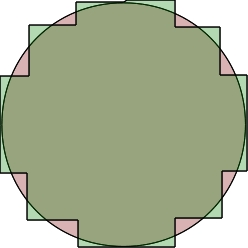
\includegraphics[keepaspectratio, width = 1.25 in]{images/squarecylinder}
    \end{center}
    \caption{A reentrant square cyclinder.}
    \label{fig:squarecylinder}
\end{wrapfigure}
Since $\mathbf{\hat{n}} \cdot \mathbf{\Omega}$ is just the cosine of the angle between the incident neutrons and the normal vector, we see the flux vanishes whenever that cosine is negative, or whenever the neutron direction is inward.

A point of warning: reentrant geometries must be avoided when using vacuum conditions.  Unless treated with special care, reentrant geometries lead to inconsistency.  Neutrons leaving one portion of the geometry could, in theory, reenter another portion, but since vacuum conditions disallow this, the true problem is not modeled correctly.  A common example of this occurs when ``squaring'' an exterior cylindrical boundary, as exhibited in Figure \ref{fig:squarecylinder}.

Another useful boundary condition is simply to specify the incident flux when it is known:
\begin{equation}
 \psi(\mathbf{r}_s,\mathbf{\Omega},E,t) = f(\mathbf{r}_s,\mathbf{\Omega},E,t) \, .
\end{equation}
In this way, boundary sources can be defined.

A \textit{reflective} or \textit{specular} condition is such that 
\begin{equation}
 \psi(\mathbf{r}_s,\mathbf{\Omega},E,t) = \psi(\mathbf{r}_s,\mathbf{\Omega}_R,E,t) \, , \, \, \, \,  \, \, \, \mathbf{\hat{n}} \cdot \mathbf{\Omega} < 0 \, ,
\end{equation}
where $\mathbf{\Omega}_R$ is the (mirror) reflection of $\mathbf{\Omega}$.  Reflective conditions are widely used in lattice physics, where pin cells or assemblies are modeled in an infinite array; the ``infinite'' is captured by the reflective conditions.  See Figure \ref{fig:reflectiveperiodic}.

A variation on reflective conditions is an \textit{albedo} condition, where
\begin{equation}
 \psi(\mathbf{r}_s,\mathbf{\Omega},E,t) = \alpha \psi(\mathbf{r}_s,\mathbf{\Omega}_R,E,t) \, , \, \, \, \,  \, \, \, \mathbf{\hat{n}} \cdot \mathbf{\Omega} < 0 \, .
\end{equation}
Here, $\alpha$ is the ``albedo'' and quantifies the strength with which neutrons stream back into the system after streaming out.  Historically, albedo conditions were highly useful since they can often capture the physics of reflectors with minimum computational cost.  The albedos for many materials were precomputed (or found experimentally), effectively eliminating a significant portion of phase space in e.g. reactor analysis.

Another approach is to use \textit{periodic} conditions, such that
\begin{equation}
 \psi(\mathbf{r}_1,\mathbf{\Omega},E,t) = \psi(\mathbf{r}_2,\mathbf{\Omega},E,t) \, ,
\end{equation}
Figure \ref{fig:reflectiveperiodic} illustrates both reflective and periodic boundary conditions.  Periodic conditions work well in infinite arrays that have assymetric unit cells (for which reflective conditions would represent an infinite but incorrect array).

\begin{figure}[h] 
    \centering
    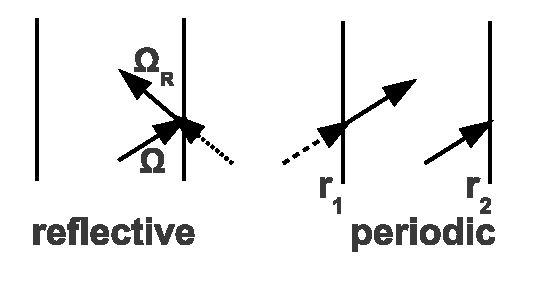
\includegraphics[keepaspectratio, width = 2.0 in]{images/reflectiveperiodic}
    \caption{Reflective and periodic boundary conditions.}
    \label{fig:reflectiveperiodic}
\end{figure}

The final boundary condition we mention is the \textit{white boundary condition}, a condition where all neutrons incident on a boundary reflect back isotropically in angle.  For this case,
\begin{equation}
\begin{split}
 \psi(\mathbf{r}_s,\mathbf{\Omega},E,t) &= \frac{ \int_{\mathbf{\hat{n}} \cdot \mathbf{\Omega}' > 0}   \mathbf{\hat{n}} \cdot \mathbf{\Omega}' \psi (\mathbf{r},\mathbf{\Omega}',E,t)d\Omega' } {  \int_{\mathbf{\hat{n}} \cdot \mathbf{\Omega}' > 0}  \mathbf{\hat{n}} \cdot \mathbf{\Omega}'  d\Omega'    }  \\
             &= \frac{ J_+ (\mathbf{r}_s,E,t) } {  \int_{\mathbf{\hat{n}} \cdot \mathbf{\Omega}' > 0}  \mathbf{\hat{n}} \cdot \mathbf{\Omega}'  d\Omega'    }\, , \, \, \, \,  \, \, \, \mathbf{\hat{n}} \cdot \mathbf{\Omega}' < 0 \, .
\end{split}
\end{equation}
Note the conditions on $\mathbf{\Omega}$ and $\mathbf{\Omega}'$.  The first corresponds to the left hand side and is limited to $\mathbf{\hat{n}} \cdot \mathbf{\Omega}' < 0$, i.e. incoming directions.  Contrarily, $\mathbf{\Omega}'$ is the dummy variable on the right hand side, and is always integrated over the domain where $\mathbf{\hat{n}} \cdot \mathbf{\Omega}' > 0$, i.e. outgoing directions.  This is so because we integrate the entire outgoing neutron population (which is proportional to the outgoing partial current) and then redistribute that number uniformly over all incident directions, i.e. isotropically.

White boundary conditions have had use in lattice physics where an isotropic angular distribution is sometimes relatively accurate.  In particular, the white boundary condition provides a useful fix for reflective conditions in Wigner-Seitz cells, which convert square pin cells into equivalent cylindrical cells, since cylindrical cells can be treated with 1-d methods.  However, while in square cells the reflective conditions work fine, they do not work well in cylindrical geometries (see Figure \ref{fig:wignerseitz}), since neutrons entering at certain angles can spend too much time in the moderator before colliding.  This consequently leads to overprediction of the moderator flux, an artifact known as the Newmarch effect. As a result, white conditions are used.


\begin{figure}[h] 
    \centering
    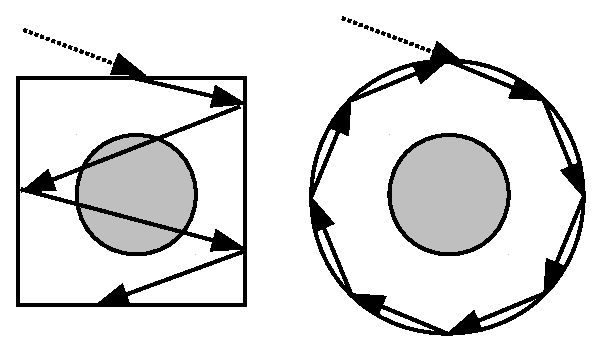
\includegraphics[keepaspectratio, width = 3.0 in]{images/wignerseitz}
    \caption{Square pin cell and equivalent Wigner-Seitz cell.  Same incident direction and location.}
    \label{fig:wignerseitz}
\end{figure}

\section*{Other Transport Equations}

We finish this lecture by presenting in brief two other important transport equations.

\subsection*{Photon Transport}

Photon transport is fundamental to radiation hydrodynamics (an integral aspect of ``bomb'' physics) and astrophysics.  Photon transport can largely be divided into two classes of problems: \textit{radiative transfer}, which consists of the propogation of soft (low energy) x-rays, and \textit{high energy} photon transport, which can largely be treated as we do neutrons.  We briefly describe the former.

The quantity of interest is the intensity, essentially an ``energy angular flux'', and is defined
\begin{equation}
 I_{\nu}(\mathbf{r},\mathbf{\Omega},t) = (h\nu)cn(\mathbf{r},\mathbf{\Omega},E,t) \, ,
\end{equation}
where $h\nu$ is the photon energy.  The ``radiative transfer equation'' is
\begin{equation}
 \frac{1}{c}\frac{\partial I_{\nu}}{\partial t} + \Omega \cdot \nabla I_{\nu} = \rho(\varepsilon_{\nu} - \kappa_{\nu}I_{\nu}) \, ,
 \label{eq:radiative}
\end{equation}
where $\varepsilon$ is a mass emission coefficient (a source term), and $\kappa$ is a mass attenuation coefficient (a loss term).  The radiative transfer equations are nonlinear due to the temperature-dependence of the underlying interaction coefficients (the ``cross-sections), particularly the emission term (which is not explicitly represented in Eq. \ref{eq:radiative}).

For the case of local thermodynamic equilibrium (LTE), Eq. \ref{eq:radiative} is simplified somewhat.  Local thermodynamic equilibrium exists when the quantity $S_{\nu} = \varepsilon_{\nu}/\kappa_{\nu} = B_{\nu}$, where $B_{\nu}$ is the Planck distribution (i.e. the black body spectrum).  In this case, Eq. \ref{eq:radiative} takes the form
\begin{equation}
 \frac{1}{c}\frac{\partial I_{\nu}}{\partial t} + \Omega \cdot \nabla I_{\nu} = \rho \kappa_{\nu} (B_{\nu} - I_{\nu}) \, .
 \label{eq:radiativelte}
\end{equation}

Radiative transfer is inherently a frequency-dependent process: the coefficients depend on the frequency, and a medium emits photons of a wide range of frequencies.  A frequently used approximation is to neglect this dependence in what is called the \textit{grey approximation}, similar to the one-speed studies in neutron transport we will study in the next several lectures.  ``Black bodies'' are also often used; these are pure absorbers whose emission spectrum is the Planck distribution.

To determine the temperature (dependence on which is implicit in all the quantities of Eq. \ref{eq:radiative}), an energy conservation equation is used.  As an example, using the grey approximation and assuming temperature- and spatially-independent coefficients, Eq. \ref{eq:radiative} becomes
\begin{equation}
 \frac{1}{c}\frac{\partial I}{\partial t} + \Omega \cdot \nabla I(\mathbf{r},\mathbf{\Omega},t) = \rho \kappa (acT^4(\mathbf{r},t)- I) \, ,
 \label{eq:radiativegrey}
\end{equation}
where $a$ is the emissivity (as in the Stefan-Boltzmann law) and $T$ is the temperature.  The corresponding energy conservation equation is
\begin{equation}
 \overbrace{c_v \frac{\partial T}{\partial t}}^{\text{energy rate of change}} = \overbrace{\rho \kappa}^{\text{abs. coef.}} \overbrace{\int_{4\pi} I(\mathbf{r},\mathbf{\Omega},t) d\Omega}^{\text{energy flux}} - \overbrace{\rho \kappa a c T^4(\mathbf{r},t)}^{\text{loss due to emission}} + \overbrace{Q(\mathbf{r},t)}^{\text{gains from outside}} \, ,
\end{equation}
where $c_v$ is the specific heat and $Q$ represents any external energy source.


\subsection*{Plasma Transport}

Another area of interest for nuclear engineers is plasma physics.  Let us apply Eq. \ref{eq:generalte} to electrons in a plasma, where we substitute in the Lorentz force for $\mathbf{F}$:
\begin{equation}
  \frac{\partial n}{\partial t} 
   + \mathbf{v} \cdot \nabla n + \frac{e}{m} \Big ( \mathbf{E}+(\mathbf{v}\times \mathbf{B} ) \Big ) \cdot \nabla_{\mathbf{v}} n =   \Big( \frac{\partial n}{\partial t} \Big )_{\mathrm{coll}} +  s \, .
\end{equation}
If we neglect sources and collisions, we arrive at the Vlasov equation:
\begin{equation}
  \frac{\partial n}{\partial t} 
   + \mathbf{v} \cdot \nabla n + \frac{e}{m} \Big ( \mathbf{E}+(\mathbf{v}\times \mathbf{B} ) \Big ) \cdot \nabla_{\mathbf{v}} n =  0 \, .
\end{equation}
Augmented with Maxwell's equations, the Vlasov equation gives a rather complete description of collisionless plasmas.  

\section*{Further Reading}

The treatment of boundary conditions is rather straightforward, but the student may wish to consult e.g. Duderstadt and Martin \cite{duderstadt1976tt} or Lewis and Miller \cite{lewis1993cmn}.  The discussion of white boundary conditions and the Wigner-Seitz dilemma follows that of H\'{e}bert \cite{hebert2009arp}, and the Newmarch effect is identified by Stamm'ler and Abbate \cite{stammler1983mss}.   

The discussion of photon and plasma transport largely follows that of Duderstadt and Martin \cite{duderstadt1976tt}.  The example grey approximation equations are given in a paper by Miller and Lewis \cite{miller1987nrm}, and there is a wealth of literature on the subject.  For those interested in radiative transfer as it applies to atmospheres, see MIT course 12.815.




% \chapter{Analytical Solutions}
\label{lec:analytical}

In this lecture, we analyze the neutron transport equation analytically for several simple cases.  In particular, we investigate neutron streaming in a vacuum and in a purely absorbing slab.  The next lecture offers further analytical and semi-analytical treatments using the integral form of the transport equation.  These two lectures ultimately show the difficulty with which realistic problems can be addressed by ``pen and paper'' and serve to motivate our later discussions of deterministic numerical methods.

\section*{One-Speed Transport}

Before we consider solutions to the transport equation, we first eliminate the energy dependence.  The reason for this is simple: \textit{the energy is simply too hard to deal with directly}.  The dependence of the various cross-sections on the energy is erratic, and, as we have seen in previous lectures, there are isotopes whose dependence on energy in certain energy ranges cannot even be resolved!

We can eliminate $E$ in two ways.  First, we can assume that $\psi$ and the cross-sections are constant in energy within an energy range $E_g < E < E_{g-1}$; this is the multi-group method, which has been the workhorse of deterministic transport methods for decades\footnote{A new methodology being developed here at MIT is a generalization of the multigroup method where instead of flat fluxes within groups (a ``zeroth`` order representation), the fluxes can have higher order dependences (linear, parabolic, etc.) using discrete Legendre polynomial expansions.}.  A second, somewhat superficial approach is to multiply the energy-dependent transport equation by $\delta(E-E_0)$.   Since $f(x)\delta(x-x_0) = f(x_0)$, we have for $E_0$ (or a groups $g$) the time- and energy-independent or \textit{one-speed transport equation}:
\begin{equation}
     \hat{\Omega} \cdot \nabla \psi(\mathbf{r},\mathbf{\Omega})  + \Sigma_t \psi(\mathbf{r},\mathbf{\Omega}) =   \int_{4\pi} d\Omega' \Sigma_s(\mathbf{r},\mathbf{\Omega}\cdot\mathbf{\Omega}')\psi(\mathbf{r},\mathbf{\Omega'}) + s(\mathbf{r},\mathbf{\Omega})  \, .
\end{equation}

\section*{Streaming in Vacuum}

Perhaps the easiest class of problems to consider are those whose medium is vacuum.  In this case, there are no particle interactions, and all we need to do is follow particles along trajectories from sources.  These trajectories are called \textit{characteristics}, and in general, the \textit{method of characteristics} is the mathematical technique we can use to find $\psi$.  Note, a more general use of the \textit{method of characteristics} applies to arbitrary media and is fast becoming the standard transport method in lattice physics.

\section*{The Streaming Term}

Consider the streaming of neutrons in a sourceless vacuum:
\begin{equation}
     \hat{\Omega} \cdot \nabla \psi(\mathbf{r},\mathbf{\Omega}) =   0  \, .
\end{equation}
What form does the streaming term $ \hat{\Omega} \cdot \nabla \psi $ have?  It depends crucially on the underlying coordinate systems.  

It helps to note that  $\mathbf{\hat{\Omega}} \cdot \nabla \psi$ is just the spatial rate of change of $\psi$ along the direction of travel, i.e. along the characteristic.  Suppose we have a particle originally at a location $\mathbf{r}_0$  going in a direction $\mathbf{\Omega}$.  Then upon traveling a distance $s$, the location $\mathbf{r} = \mathbf{r}_0 + s\mathbf{\Omega}$.  Accordingly, the spatial rate of change of $\psi$ can be written
\begin{equation}
    \frac{d}{ds} \psi(\mathbf{r}_0 +s\mathbf{\Omega},\mathbf{\Omega}) =   0  \, .
    \label{eq:spaceratepsi}
\end{equation}

We can also show more explicitly that $\frac{d\psi}{ds} = \hat{\Omega} \cdot \nabla \psi$.  In general, the direction vector $\mathbf{\Omega}$ has the basic form
\begin{equation}
 \mathbf{\Omega} = \mu \mathbf{\hat{e}}_{\mu} + \eta \mathbf{\hat{e}}_{\eta} + \xi \mathbf{\hat{e}}_{\xi} \, ,
\end{equation}
where $\mu$, $\eta$, and $\xi$ are directional cosines and the $\mathbf{\hat{e}}$'s are corresponding coordinate vectors.  In general, $\mathbf{\Omega}$ depends on three spatial coordinates $p_1$, $p_2$, and $p_3$ and two angular coordinates, usually parameterized as the cosine of the polar angle $\chi = \cos(\theta)$\footnote{We use $\chi$ to represent the polar angle cosine in general rather than $\mu$, since $\mu$ here will be the directional cosine with respect to the $x$ axis.} and the azimuthal angle $\phi$.  Hence,
\begin{equation}
 \frac{d}{ds} = \frac{dp_1}{ds}\frac{\partial}{\partial p_1} + \frac{dp_2}{ds}\frac{\partial}{\partial p_2} + \frac{dp_3}{ds}\frac{\partial}{\partial p_3} + \frac{d\mu}{ds}\frac{\partial}{\partial \mu} + \frac{d\phi}{ds}\frac{\partial}{\partial \phi} \, .
 \label{eq:totalsderivative}
\end{equation}
The various derivatives in Eq. \ref{eq:totalsderivative} may or may not vanish, depending on the geometry.  Consider Cartesian geometry where $p_1 = x$ and so on.  The Cartesian spatial and angular system was given in Figure \ref{fig:phase_space}, where the polar angle was defined with respect to the $z$ axis and the azimuth with respect to the $x$ axis.  Any incremental movement $ds$ along the direction $\mathbf{\Omega}$ can be seen  to change neither $\theta$ (nor its cosine $\xi$) nor $\phi$, since the angular coordinate system is invariant as the particle moves.  All this means is that $\mathbf{\Omega}$ at $\mathbf{r}_0$ is the same as the $\mathbf{\Omega}$ at $\mathbf{r}_0 + ds\mathbf{\Omega}$.  Hence, $d\xi/ds = d\phi/ds = 0$ and
\begin{equation}
 \frac{d}{ds} = \frac{dx}{ds}\frac{\partial}{\partial x} + \frac{dy}{ds}\frac{\partial}{\partial y} + \frac{dz}{ds}\frac{\partial}{\partial z} \, ,
\end{equation}
but $dx/ds$ is just the directional cosine with respect to the $x$ axis, $\mu$, and likewise $dx/ds = \eta$ and $dz/ds = \xi$ so that
\begin{equation}
 \frac{d}{ds} = \mu \frac{\partial}{\partial x} + \eta \frac{\partial}{\partial y} + \xi \frac{\partial}{\partial z} = \mathbf{\Omega} \cdot \nabla  \, .
\end{equation}

For other geometries, the streaming term is not as simple, since the angular coordinate system does depend on the position $\mathbf{r}$.  The spherical spatial and angular system is given if Figure \ref{fig:spherical_phase_space}.  The three spatial coordinates are $r$, $\theta_r$ and $\phi_r$.  The angular coordinate system is such that the polar angle is defined with respect to $\mathbf{r}$.  The azimuth and secondary coordinates are defined somewhat arbitrarily.

\begin{figure}[ht] 
    \centering
    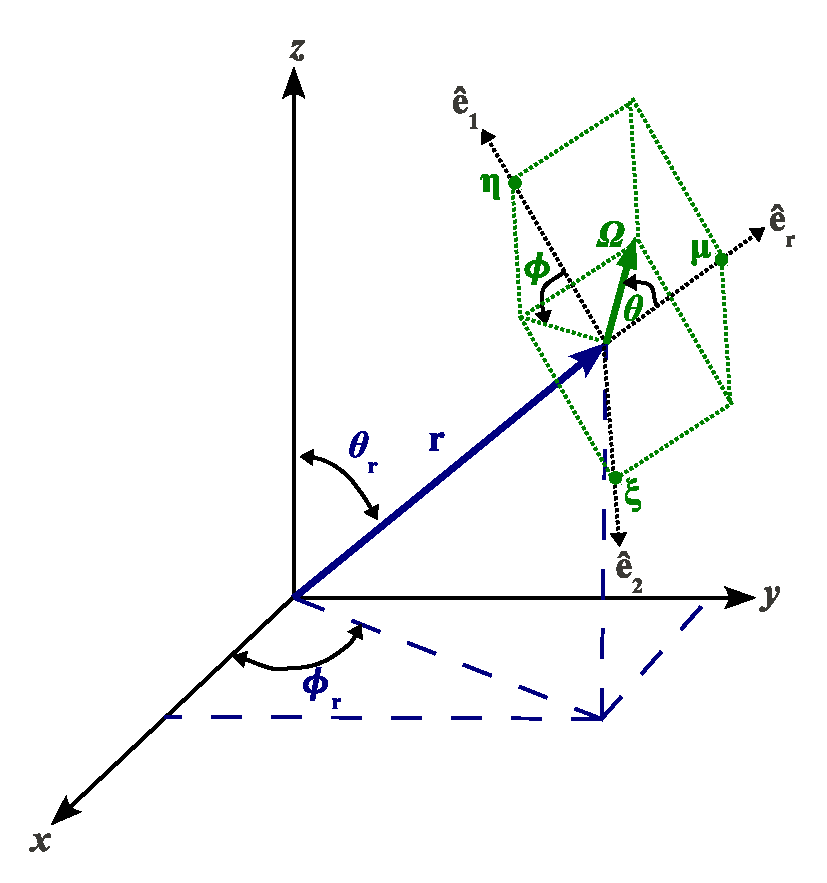
\includegraphics[keepaspectratio, width = 3.0 in]{images/spherical_phase_space}
    \caption{Spherical phase space.}
    \label{fig:spherical_phase_space}
\end{figure}

The streaming operator in spherical coordinates is defined generally as 
\begin{equation}
 \frac{d}{ds} = \frac{dr}{ds}\frac{\partial}{\partial r} + \frac{d\theta_r}{ds}\frac{\partial}{\partial \theta_r} + \frac{d\phi_r}{ds}\frac{\partial}{\partial \phi_r} + \frac{d\mu}{ds}\frac{\partial}{\partial \mu} + \frac{d\phi}{ds}\frac{\partial}{\partial \phi} \, .
\end{equation}
As a simple example, consider the case of 1-d transport in spherical coordinates, for which we assume the flux is independent of the spatial coordinates $\theta_{r}$ and $\phi_{r}$, which eliminates the derivatives with respect to $\theta_r$ and $\phi_r$.  Moreover, if we look at the angular coordinates, we see that if $r$ is the only spatial variable, then there should be dependence only on $\mu$.  A dependence on the azimuthal angle would require a non-uniform particle distribution in the other spatial directions.  Hence, the derivative with respect to $\phi$ also vanishes, leaving
\begin{equation}
 \frac{d}{ds} = \frac{dr}{ds}\frac{\partial}{\partial r} + \frac{d\mu}{ds}\frac{\partial}{\partial \mu}  \, .
\end{equation}
From Figure \ref{fig:spherical_phase_space}, we can immediately see that
\begin{equation}
 \frac{dr}{ds} = \mu \, .
 \label{eq:drds}
\end{equation}
Less obvious is $d\mu/ds$.  First note that $r d\theta = -ds \sin\theta$, which we can see directly from Figure \ref{fig:spherical_angle_with_r}.  The negative sign arises because a positive $ds$ leads to a decrease $\theta$. Then, noting that $\mu = \cos{\theta}$ so that $d\mu = -\sin{\theta} d\theta$, we can show
\begin{equation}
 \frac{d\mu}{ds} = \frac{1-\mu^2}{r} \, ,
 \label{eq:dmuds}
\end{equation}
and
\begin{equation}
 \frac{d\psi}{ds} = \mathbf{\Omega} \cdot \nabla_{\text{1d}} \psi = \mu \frac{\partial \psi}{\partial r} +  \frac{1-\mu^2}{r}\frac{\partial \psi}{\partial \mu} \, .
\end{equation}


\begin{figure}[ht] 
    \centering
    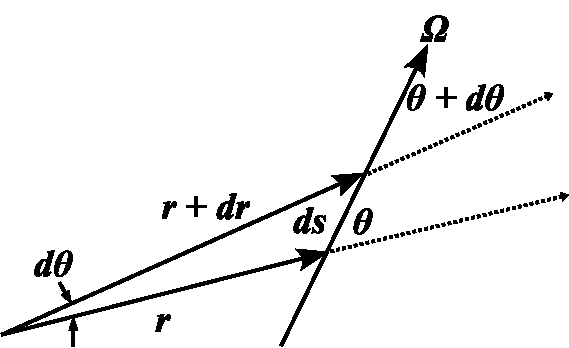
\includegraphics[keepaspectratio, width = 2.5 in]{images/spherical_angle_with_r}
    \caption{Change in $r$ and $\theta$ as a particle streams.}
    \label{fig:spherical_angle_with_r}
\end{figure}


\section*{Example 1: Meandering from a Plane Source in a Vacuum Slab}

As a first example, consider the case of neutrons streaming in a 1-d slab for $x>0$ where the source is an isotropic planar source at $x=0$ which we will use as a boundary condition rather than a source term. The Cartesian streaming term above simplifies in 1-d to
\begin{equation}
 \mu \frac{\partial \psi}{\partial x} = 0 \, ,
\end{equation}
subject to
\begin{equation}
 \psi(0,\mu) = \frac{S_0}{2} \, .
\end{equation}
In 1-d slab geometry, we essentially integrate out the 2$\pi$ associated with the azimuthal angle.  Hence, isotropic sources of strength $S$ become $S/2$ instead of $S/4\pi$.  The units of $\psi$ are slightly different, and one must divide by $2\pi$ [rad] in order to obtain units appropriate in 3-d.  Integrating the equations shows that
\begin{equation}
 \psi(x,\mu) = c \, , \, \, \, \, \mu > 0 \, ,
\end{equation}
for some constant $c$.  At $x = 0$, we must have $\psi(0,\mu) = S/2$, and so for all $x > 0$, $\psi(x,\mu) = S/2$.  The same holds for negative $x$ and $\mu$.

\section*{Example 2: Playing in Vacuum Outside a Spherical Shell Source}

We now consider a neutrons streaming in a vacuum due to an isotropic spherical shell source of radius $r_0$.  We focus only on $r > r_0$.  The transport equation can be written
\begin{equation}
 \mu \frac{\partial \psi}{\partial r} + \frac{1-\mu^2}{r} \frac{\partial \psi}{\partial \mu} = \frac{S_0\delta(r-r_0)}{4\pi r_0} \, .
\end{equation}
From Eqs. \ref{eq:drds} and \ref{eq:dmuds}, we have
\begin{equation}
 ds = \frac{d\mu}{ (1-\mu^2)/r } = \frac{dr}{\mu} \, ,
\end{equation}
or
\begin{equation}
 \frac{dr}{r} = \frac{\mu d\mu}{1-\mu^2} \, .
\end{equation}
We integrate from initial coordinates $r_s$ and $\mu_s$, as shown in Figure \ref{fig:sphere_example}, and rearrange to obtain
\begin{equation}
 \mu = \sqrt{ 1 - (1-\mu^2_s)\Big (\frac{r_s}{r} \Big )^2  } \, .
 \label{eq:angularrestribution}
\end{equation}
\begin{figure}[ht] 
    \centering
    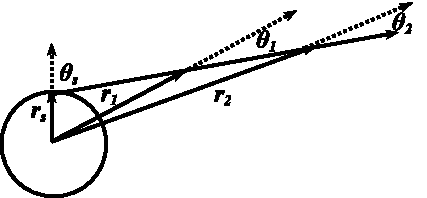
\includegraphics[keepaspectratio, width = 2.5 in]{images/sphere_example}
    \caption{Streaming of particles from spherical shell source.}
    \label{fig:sphere_example}
\end{figure}

Eq. \ref{eq:angularrestribution} shows explicitly how $\mu$ changes as a function of $r$.  This phenomenon is often called angular redistribution and leads to collimation of the flux away from the source.  Since $d\psi/ds$ must equal the source, we can write
\begin{equation}
 ds = \frac{d\mu}{ (1-\mu^2)/r } = \frac{d\psi}{ \frac{S_0\delta(r-r_0)}{4\pi r_0}  } \, ,
\end{equation}
or 
\begin{equation}
\frac{d\psi}{dr} = \frac{S_0\delta(r-r_0)}{4\pi r_0} \, .
\end{equation}
Then
\begin{equation}
 \int^{r,\mu}_{r_s,\mu_s} \frac{d\psi}{dr}  = \int^r_{r_s} dr \frac{S_0\delta(r-r_0)}{4\pi r_0} \, ,
\end{equation}
or
\begin{equation}
 \psi(r,\mu)-\psi(r_s,\mu_s) = \frac{S_0}{8\pi r^2_s} \frac{1}{\sqrt{1-(1-\mu^2_s)}} \, .
\end{equation}
We take the boundary flux to be $\psi(r_s,\mu_s) = 0$, which implies that $\mu_s$ is limited to $\mu_s \leq 0 \leq \pi/2$. If $\mu_s$ spanned through $\pi$, then particles could be born into the sphere and stream out of another location, a complication we care to avoid in this example.  From Eq. \ref{eq:angularrestribution}, we have $(1-\mu^2_s)=(r/r_s)^2(1-\mu^2)$.  We note that for $\mu_s = 0$, $\mu=\sqrt{1-(r_s/r)^2}$ and when $\mu_s=1$, $\mu=1$.  Finally, we have
\begin{equation}
 \psi(r,\mu) = \frac{S_0}{8\pi} \frac{1}{\sqrt{r^2_s - r^2(1-\mu^2)}} \, , \, \, \, \, \, \sqrt{1-\Big ( \frac{r_s}{r} \Big )^2 } \leq \mu \leq 1 \, .
 \label{eq:spherepsi}
\end{equation}

To illustrate the behavior of $\psi$, we have taken $r_s = 1$ and $S_0 = 8\pi$.  Figure \ref{fig:sphere_psi_radius} shows $\psi$ as a function of radius for several $\mu$ values.  Of course, we see that as neutrons move farther from the source, the flux at larger $\theta$ values (smaller $\mu$ values) diminishes, as we expect due to angular redistribution. Figure \ref{fig:sphere_psi_mu} shows $\psi$ as a function of $\mu$ for several values of $r$.  We see effects of the same phenomenon, in that the angular distribution becomes more collimated about $\mu = 1$ for larger $r$.
\begin{figure}[ht] 
    \centering
    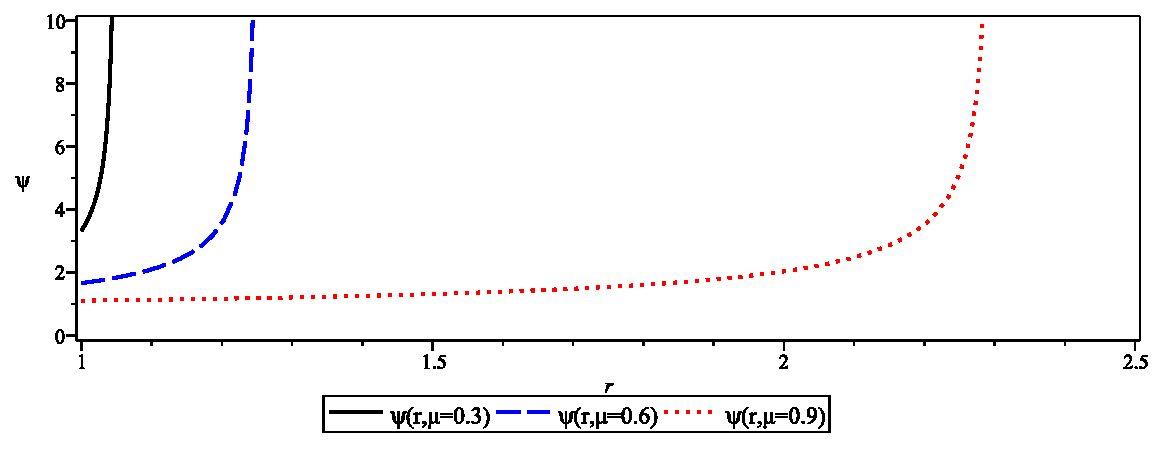
\includegraphics[keepaspectratio, width = 5.0 in]{images/sphere_psi_radius}
    \caption{Angular flux as a function of radius for certain $\mu$ values.}
    \label{fig:sphere_psi_radius}
\end{figure}

\begin{figure}[ht] 
    \centering
    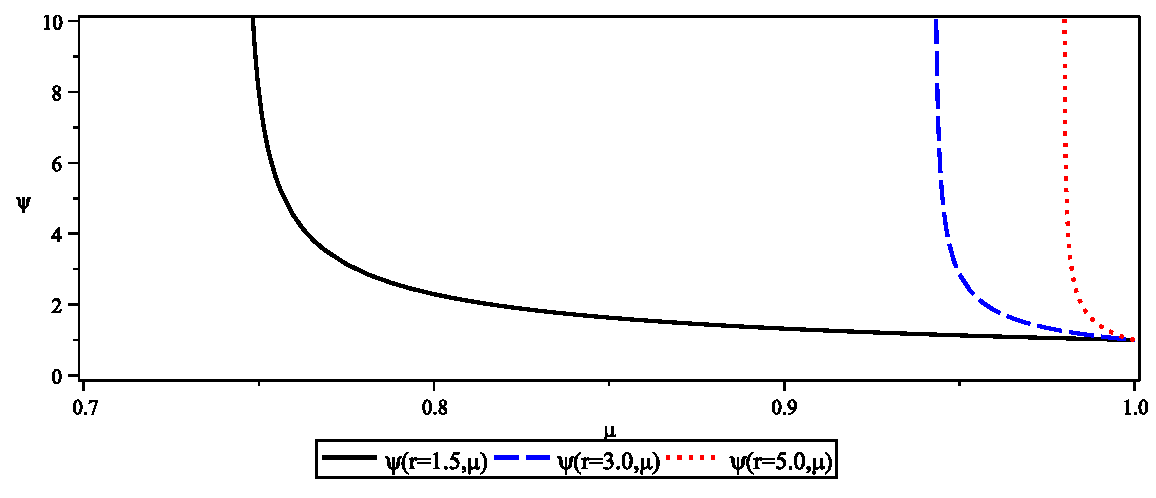
\includegraphics[keepaspectratio, width = 5.0 in]{images/sphere_psi_mu}
    \caption{Angular flux as a function of $\mu$ at certain $r$ values.}
    \label{fig:sphere_psi_mu}
\end{figure}

\section*{Example 3: A Purely Absorbing Slab}

As a final example, we apply what we've learned in vacuum to transport in a purely absorbing slab.  In this case, the 1-d transport equation is
\begin{equation}
 \mu \frac{\partial \psi}{\partial x} + \Sigma_a(x)\psi(x,\mu) = S(x,\mu) \, .
\end{equation}
As an example, we study a uniform slab of length $L$, subject to vacuum boundaries, and with a uniform, isotropic source of volumetric strength\footnote{By volumetric strength, we mean the units are neutrons per unit volume per second.} $S_0$.  Our equation simplifies to 
\begin{equation}
 \mu \frac{\partial \psi}{\partial x} + \Sigma_a \psi(x,\mu) = \frac{S_0}{2} \, .
 \label{eq:slababsorber}
\end{equation}
To solve the problem, we decompose $\psi$ into $\psi_+$ for $\mu > 0$ and $\psi_-$ for $\mu < 0$.  In this way, we can start at one end of the slab and work our way across, essentially as would a neutron.

For $\mu>0$, we divide Eq. \ref{eq:slababsorber} through by $\mu$ and compute the integrating factor
\begin{equation}
 if = \exp{\int^x_0 dx \Sigma_a\mu} = \exp{\Sigma_a x/\mu} \, .
\end{equation}
Then we have
\begin{equation}
 \frac{d}{dx}\Big ( \psi_{+} e^{\Sigma_a x} \Big ) = \frac{S_0}{2\mu}  e^{\Sigma_a x/\mu} \, ,
\end{equation}
and integrating from $0$ to $x$ yields
\begin{equation}
 \psi_{+} = \frac{S_0}{2\Sigma_a}\Bigg (1 - e^{-\Sigma_a x/\mu} \Bigg ) \, ,
\end{equation}
where we note $\psi_+{0,\mu} = 0$ from the given boundary condition.

For $\mu<0$, we do similarly.  It helps in this case to use $-|\mu|$ in place of $\mu$, as it can be easy to lose negative signs.  Using the integrating factor $\exp{(L-x)/|\mu|}$, we find after integrating from $L$ to $x$ that
\begin{equation}
 \psi_{-} = \frac{S_0}{2\Sigma_a}\Bigg (1 - e^{-\Sigma_a (L-x)/|\mu|} \Bigg ) \, .
\end{equation}
For the case of $L = 10$ and $\Sigma_a = 1$, Figure \ref{fig:slab_example_psi} shows $\psi$ for several values of $\psi$.  Note the symmetry, as should be expected. 

\begin{figure}[ht] 
    \centering
    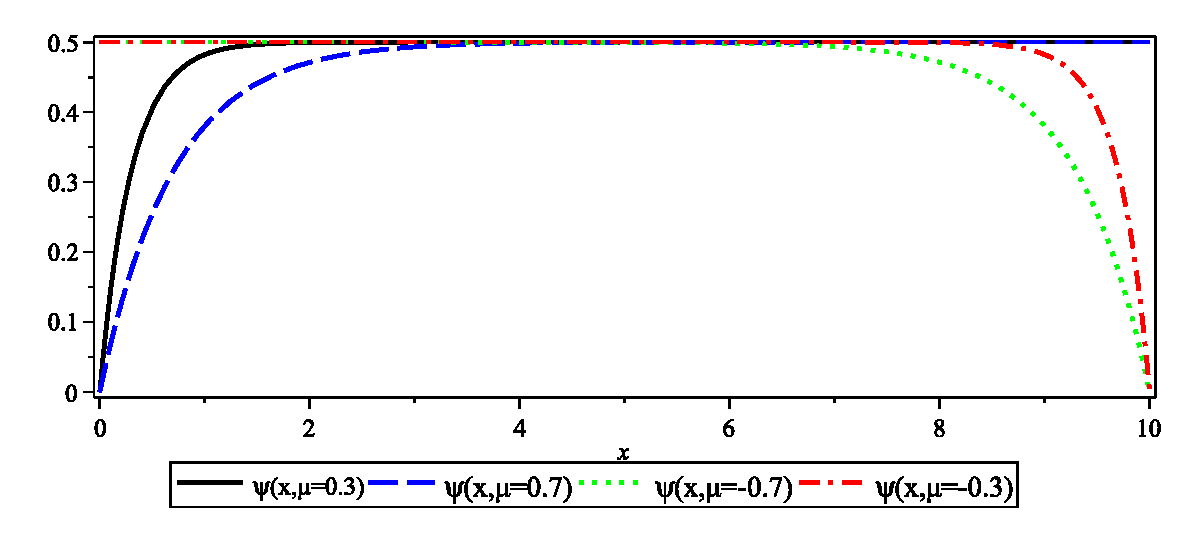
\includegraphics[keepaspectratio, width = 5.0 in]{images/slab_example_psi}
    \caption{Angular flux at specific angles for the absorbing slab.}
    \label{fig:slab_example_psi}
\end{figure}

Our next goal is to compute the scalar flux.  By definition, the scalar flux in 1-d is
\begin{equation}
 \phi(x) = \int^1_{-1} d\mu \psi(x,\mu) \, ,
\end{equation}
which can be broken into
\begin{equation}
  \phi(x) = \int^0_{-1} d\mu \psi_{-}(x,\mu) + \int^1_{0} d\mu \psi_{+}(x,\mu) \, .
\end{equation}
Inserting our expressions above, we have
\begin{equation}
\begin{split}
  \phi(x) &= \frac{S_0}{2\Sigma_a} \Bigg (  \int^{1}_{-1} d\mu - \int^0_{-1} d\mu  e^{-\Sigma_a (L-x)/|\mu|} - \int^1_{0} d\mu e^{-\Sigma_a x/\mu}  \Bigg ) \\
          &= \frac{S_0}{2\Sigma_a} \Bigg ( 2 - \int^1_{0} d\mu'  e^{-\Sigma_a (L-x)/\mu} - \int^1_{0} d\mu e^{-\Sigma_a x/\mu}  \Bigg ) \\
          &= \frac{S_0}{2\Sigma_a} \Bigg ( 2 - E_2(\Sigma_a (L-x)) - E_2(\Sigma_a x)  \Bigg ) \, .
\end{split}
\end{equation}
For the same numerical example, $\phi(x)$ is shown in Figure \ref{fig:slab_example_phi_current} along with the current density $\mathbf{J}(x)$, computation of which is left as an exercise.

\begin{figure}[ht] 
    \centering
    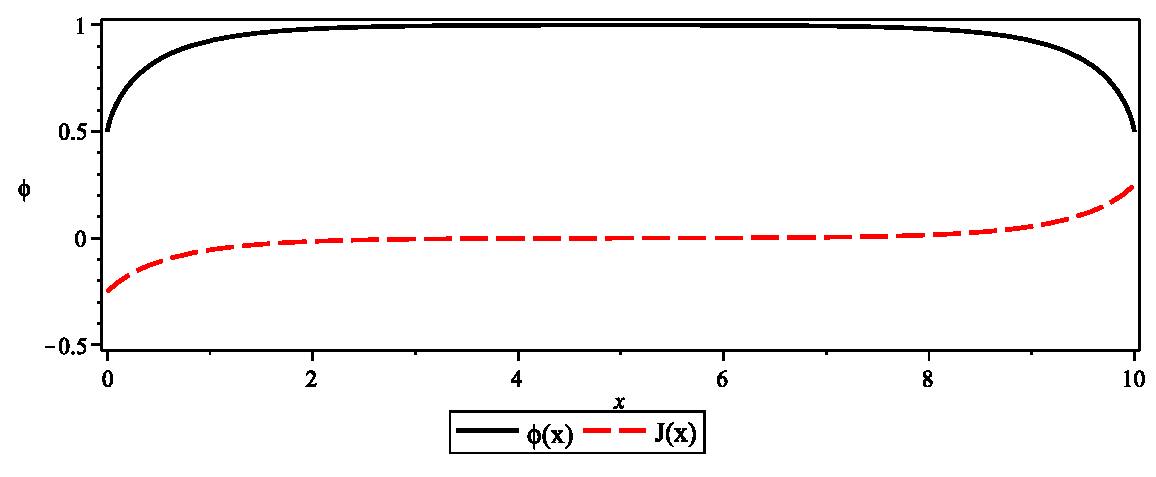
\includegraphics[keepaspectratio, width = 5.0 in]{images/slab_example_phi_current}
    \caption{Scalar flux and current density.}
    \label{fig:slab_example_phi_current}
\end{figure}

\section*{Exponential Integrals}

The functions $E_n(x)$ are called ``exponential integrals'' and are characteristic of slab problems.  They are defined by
\begin{equation}
 E_n(x) \equiv \int^1_0 d\mu \mu^{n-2} e^{-x/\mu} \, .
 \label{eq:EnDefinition}
\end{equation}
They also satisfy
\begin{equation}
 E_n(x) = - \int dx E_{n-1}(x) \, .
 \label{eq:EnIntegration}
\end{equation}
Several of the $E_n$ functions are shown in Figure \ref{fig:slab_example_exp_functions}.

\begin{figure}[ht] 
    \centering
    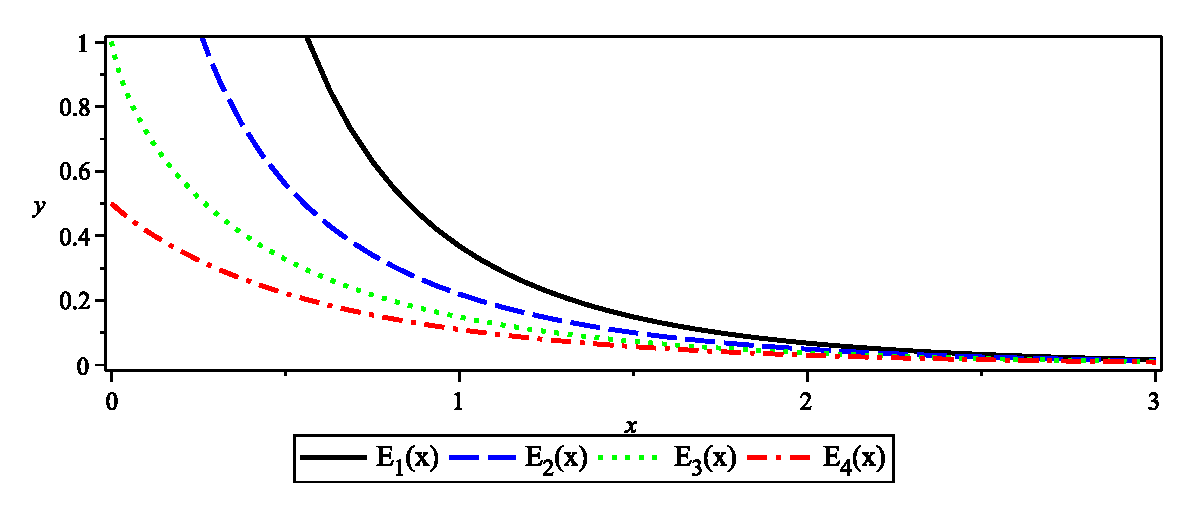
\includegraphics[keepaspectratio, width = 5.0 in]{images/slab_example_exp_functions}
    \caption{The first four exponential integral functions.}
    \label{fig:slab_example_exp_functions}
\end{figure}

\section*{Further Reading}

The problems discussed in this lecture have been rather elementary in nature.  To explore more realistic problems---even just including scattering in slab geometry---would take us into a much more complicated mathematical domain involving integral transforms (with inverses using complex analysis), singular eigenfunction expansions, and more.  Duderstadt and Martin \cite{duderstadt1976tt} cover most of what has been discussed, and much more.  The motivated student should look to that work (specifically Chapter 2), along with Bell and Glasstone (Chapter 2), Case and Zweifel \cite{case1967ltt}, and Davison \cite{davison1957ntt}.  These are listed in reverse chronological order, and perhaps, in increasing order of difficulty.  Davison in particular uses older notation, so the reader be aware!

\begin{exercises}

  \item \textbf{Cylindrical Coordinates}. Derive the streaming term for the neutron transport equation in 1-d cylindrical geometry.  Include diagrams to help explain your approach.
  
  \item \textbf{Angular Current from Plane Source}. In Example 1, what is the angular current $\mathbf{j}$?

  \item \textbf{Isotropic Current Conditions}. For Example 1, find $\psi$ and $\mathbf{j}$ when the boundary condition is an isotropic angular current (rather than an isotropic angular flux).

  \item \textbf{Flux Inside a Sphere}. Solve for the angular flux on the interior of the spherical shell from Example 2.

  \item \textbf{Angular Redistribution in 1-d}. Explain in your own words why $\psi$ in a 1-d spherical problem depends only on the radius $r$ and cosine of the polar angle $\mu$.  Specifically, why is there no dependence on a second angular variable? 

  \item \textbf{Scalar Flux from Spherical Shell Source}. Solve for the scalar flux on the outside of the sphere in Example 2, i.e. integrate Eq. \ref{eq:spherepsi} over $\mu$.  What happens at $r = r_s$ and why?  What is the limiting behavior of $\phi(r)$ as $r\to \infty$?  In other words, what does the spherical source ``look like'' far from its surface?

  \item \textbf{Current Density in a Slab}. Derive an expression for the current density $\mathbf{J}$ for a purely absorbing slab.  Using the values from the example, generate the curves in Figure \ref{fig:slab_example_phi_current}.  Compute the total absorption rate in the slab and the leakage rate at the boundaries.  Is it what you expect?

\end{exercises}

% \chapter{The Integral Form}

In this lecture we consider the integral form of the transport equation in both general coordinates and the specific case of slab geometry.  The integral form is useful in situations where only the scalar flux is required and is the foundation for the collision probabability method, which we cover in the next lecture, as well as the method of characteristics, fast becoming the technique of choice in reactor analysis.  We consider some analytical aspects of the integral equation and finish by discussing a simple numerical approach based on Neumann series expansions.

\section*{The Integral Transport Equation}

You may have noticed from the previous two lectures that the angular dependence of the particle density is a relatively unique aspect of transport processes.  Often, this angular dependence is the hardest aspect that we deal with directly, either analytically or numerically\footnote{Energy is by far more complex, as we've noted, and there are very few analytical problems where energy can be handled directly (slowing down in an infinite homogeneous medium problem is one example). Consequently, we typically use only the crudest representation possible in discretizing the energy variable, though much physics goes into generating the discrete data.}  It would be nice to eliminate the angular variable completely, and for certain problems, the \textit{ integral transport equation} allows us to do with a minimum of approximation.

Before we derive the integral form of the transport equation, it helps define a new quantity called the \textit{emission density},
\begin{equation}
  Q(\mathbf{r},\mathbf{\Omega}) = \int_{4\pi} d\Omega' \Sigma_s(\mathbf{r},\mathbf{\Omega}\cdot\mathbf{\Omega}')\psi(\mathbf{r},\mathbf{\Omega'}) + S(\mathbf{r},\mathbf{\Omega}) \, .
  \label{eq:emissiondensity}
\end{equation}
Essentially, $Q$ is a generalized source containing any external source $S$ and scattering source; of course, fission could also be included.

Recall the discussion of Eq. \ref{eq:spaceratepsi}, where we consider a distance $s$ from some reference point $\mathbf{r}_0$ along the characteristic $\mathbf{r}_0 +s\mathbf{\Omega}$.  The full transport equation in terms of $s$ is 
\begin{equation}
    \frac{d}{ds} \psi(\mathbf{r}_0 +s\mathbf{\Omega},\mathbf{\Omega}) + \Sigma_t(\mathbf{r}_0 +s\mathbf{\Omega})\psi =   Q(\mathbf{r}_0 +s\mathbf{\Omega},\mathbf{\Omega})  \, ,
    \label{eq:forchareq}
\end{equation}
which can be called the \textit{forward characteristic} equation, as we follow neutrons forward from the reference point.  Similar, and which we use below, is the \textit{backward characteristic} form, which represents following neutrons backward along the characteristic from a current point $\mathbf{r}$.  Let $p = -s$.  Then $d/dp = -d/ds$ and Eq. \ref{eq:forchareq} becomes (after dropping the $0$ subscript from $\mathbf{r}$)
\begin{equation}
    -\frac{d}{dp} \psi(\mathbf{r} - p\mathbf{\Omega},\mathbf{\Omega}) + \Sigma_t(\mathbf{r} -p\mathbf{\Omega})\psi =   Q(\mathbf{r} -p\mathbf{\Omega},\mathbf{\Omega})  \, .
    \label{eq:backchareq}
\end{equation}
We wish to integrate from $p=0$ to some maximum distance (eventually to be either infinity or a global boundary).  Introducing the integrating factor
\begin{equation}
 if = e^{ -\int^p_0 \Sigma_t(\mathbf{r} -p'\mathbf{\Omega}) dp'  } \, 
\end{equation}
into Eq. \ref{eq:backchareq}, we have
\begin{equation}
    -\frac{d}{dp} \Big ( \psi(\mathbf{r}_0 - p\mathbf{\Omega},\mathbf{\Omega}) e^{ -\int^p_0 \Sigma_t(\mathbf{r} -p'\mathbf{\Omega}) dp'  } \Big ) =  Q(\mathbf{r} -p\mathbf{\Omega}) e^{ -\int^p_0 \Sigma_t(\mathbf{r} -p'\mathbf{\Omega}) dp'  } \, ,
\end{equation}
and integrating
\begin{equation}
  \begin{split}
    -\int^{\psi(p'=p)}_{\psi(p=0)}  \Bigg(  d \Big ( \psi(\mathbf{r} &- p'\mathbf{\Omega},\mathbf{\Omega})   e^{ -\int^{p'}_0 \Sigma_t(\mathbf{r} -p''\mathbf{\Omega}) dp''  } \Big ) \Bigg ) = \\
   & \int^p_0 Q(\mathbf{r} -p'\mathbf{\Omega},\mathbf{\Omega})e^{ -\int^{p'}_0 \Sigma_t(\mathbf{r} -p''\mathbf{\Omega}) dp''  }dp'   \\
  \end{split}
\end{equation}
yields
\begin{equation}
  \begin{split}
    \psi(\mathbf{r},\mathbf{\Omega}) - \psi(\mathbf{r} &- p\mathbf{\Omega},\mathbf{\Omega})e^{ -\int^{p}_0 \Sigma_t(\mathbf{r} -p''\mathbf{\Omega}) dp''  }  = \\
   & \int^p_0 Q(\mathbf{r} -p'\mathbf{\Omega},\mathbf{\Omega})e^{ -\int^{p'}_0 \Sigma_t(\mathbf{r} -p''\mathbf{\Omega}) dp''  }dp'   \, .
  \end{split}
\end{equation}

We can simplify the notation somewhat by defining the \textit{optical pathlength} $\tau$, such that
\begin{equation}
  \tau ( \mathbf{r} ,\mathbf{r} -p \mathbf{\Omega} ) = \int^p_0 \Sigma_t(\mathbf{r} -p'\mathbf{\Omega}) dp' \, . 
  \label{eq:opticalpathlength}
\end{equation}
Then, the integral equation for the angular flux becomes
\begin{equation}
  \begin{split}
    \psi(\mathbf{r},\mathbf{\Omega}) = \int^p_0 Q(\mathbf{r} -p'\mathbf{\Omega},\mathbf{\Omega})e^{-\tau(\mathbf{r},\mathbf{r}-p'\mathbf{\Omega})}dp'                         +  \psi(\mathbf{r} - p\mathbf{\Omega},\mathbf{\Omega})e^{ -\tau(\mathbf{r},\mathbf{r}-p\mathbf{\Omega}) }   \, .
  \end{split}
  \label{eq:inteqpsi}
\end{equation}

In many cases, the emission density $Q$ is assumed to be isotropic in the lab system.  In this case, we can integrate out the angular dependence and arrive at an integral equation for the scalar flux often referred to as Peierl's equation.  To do so, we let the integration bound $p$ of Eq. \ref{eq:inteqpsi} go to infinity.  We assume the second term on the right hand side to vanish (i.e. either $\psi$ vanishes at infinity, or equivalently, the optical path length $\tau(\mathbf{r},\infty)$ goes to $\infty$, and so the exponential vanishes).  

Letting $Q(\mathbf{r},\mathbf{\Omega}) = Q(\mathbf{r} -p\mathbf{\Omega})/4\pi$, and substituting $\mathbf{r}' = \mathbf{r} - p \mathbf{\Omega}$, we integrate Eq. \ref{eq:inteqpsi} over all angles to get
\begin{equation}
 \phi(\mathbf{r}) = \int_{4\pi} d\Omega \int^{\infty}_0  \frac{Q(\mathbf{r}')}{4\pi}e^{-\tau(\mathbf{r},\mathbf{r}')}dp \, .
 \label{eq:integralphiPRE}
\end{equation}
Now note that $p =|\mathbf{\Omega} p|=|\mathbf{r}-\mathbf{r}'|$, and consequently $p^2 = |\mathbf{r}-\mathbf{r}'|^2$.  Multiplying within the integrand by $1=p^2/|\mathbf{r}-\mathbf{r}'|^2$ yields
\begin{equation}
 \phi(\mathbf{r}) = \int_{4\pi} d\Omega \int^{\infty}_0  \frac{Q(\mathbf{r}')}{4\pi}e^{-\tau(\mathbf{r},\mathbf{r}')}\frac{p^2dp}{|\mathbf{r}-\mathbf{r}'|^2} \, ,
\end{equation}
and if the reader thinks this looks suspiciously like a volume integral in spherical coordinates, she would be right.  Letting $dV' = 4\pi d\Omega dpp^2$, we have
\begin{equation}
 \phi(\mathbf{r}) = \int_{V'} \frac{ Q(\mathbf{r}')e^{-\tau(\mathbf{r},\mathbf{r}')} dV'}{4\pi|\mathbf{r}-\mathbf{r}'|^2} \, .
 \label{eq:integralphi}
\end{equation}

\section*{Integral Transport in Slab Geometry}

We now look at the special case of Eq. \ref{eq:integralphi} in slab geometry, for which the emission density is a function only of $x$, i.e. $Q(\mathbf{r}) = Q(x)$.  We make use of cylindrical coordinates, with the axis taken to be $x$.  Our goal will be to integrate out the radial ($\rho$) and azimuthal ($\omega$) spatial components, leaving just the $x$ dependence. The differential volume is then
\begin{equation}
 dV' = \rho d\rho d\omega dx' ,
\end{equation}
and Eq. \ref{eq:integralphi} becomes
\begin{equation}
\begin{split}
 \phi(x) &= \int^{\infty}_{-\infty} dx' \int^{\infty}_0 d\rho \rho \int^{2\pi}_0 \frac{ d\omega' Q(x')e^{-\tau(\mathbf{r},\mathbf{r}')}}{4\pi|\mathbf{r}-\mathbf{r}'|^2} \, \\
        &= 2\pi \int^{\infty}_{-\infty}dx' \int^{\infty}_0 d\rho \rho \frac{ Q(x')e^{-\tau(\mathbf{r},\mathbf{r}')}}{4\pi |\mathbf{r}-\mathbf{r}'|^2} \, .
\end{split}
\label{eq:integralphix}
\end{equation}

We now need to express $\mathbf{r}$ and $\rho$ in terms of $x$.  Since the cross-sections (as quantified by $\tau$) are really dependent only on $x$, we can relate the full distance $|\mathbf{r}' - \mathbf{r}|$ with its projection along the $x$ axis via a directional cosine $\lambda^{-1}$ such that
\begin{equation}
 \lambda = \frac{|\mathbf{r}' - \mathbf{r}|}{|x'-x|} \, 
 \label{eq:projection}
\end{equation}
and $\tau(\mathbf{r}',\mathbf{r}) = \lambda \tau(x',x)$.  Moreover,
\begin{equation}
 |\mathbf{r}' - \mathbf{r}|^2 = \rho^2 + |x' - x|^2 \, 
\end{equation}
which, using Eq. \ref{eq:projection}, can be rewritten as
\begin{equation}
 \rho^2 = (\lambda^2 -1 )|x'-x|^2 \, ,
\end{equation}
and differentiating, we find
\begin{equation}
 \rho d\rho = \lambda d\lambda |x'-x|^2 \, .
\end{equation}
Noting that $\rho = 0$ corresponds to $\lambda = 1$, Eq. \ref{eq:integralphix} can be written in terms of $\lambda$ to give
\begin{equation}
\begin{split}
 \phi(x) &= 2\pi \int^{\infty}_{-\infty}dx' \int^{\infty}_1 \lambda d\lambda \frac{|x'-x|^2 }{4\pi|\mathbf{r}' - \mathbf{r}|^2}    Q(x')e^{-\tau(\mathbf{x},\mathbf{x}')} \\
        &= 2\pi \int^{\infty}_{-\infty}dx' \int^{\infty}_1 \lambda d\lambda \frac{1}{4\pi \lambda^2}    Q(x')e^{-\tau(\mathbf{x},\mathbf{x}')} \\       
        &=  \int^{\infty}_{-\infty} dx'\frac{1}{2} \int^{\infty}_1 \lambda d\lambda\frac{1}{\lambda}  Q(x')e^{-\tau(\mathbf{x},\mathbf{x}')} \, 
\end{split}
\end{equation}
or
\begin{equation}
 \phi(x) =  \int^{\infty}_{-\infty} dx'\frac{1}{2} E_1(\tau(\mathbf{x},\mathbf{x}'))Q(x') \, ,   
 \label{eq:integralphislab}     
\end{equation}
where we have used the $E_1$ function defined at the end of Lecture \ref{lec:analytical}.  

\section*{First-Flight Kernels}

Eq. \ref{eq:integralphislab} gives us an example of the use of a \textit{first-flight kernel} for the scalar flux, the general use of which takes the form
\begin{equation}
 \phi(\mathbf{r}) = \int d^3\mathbf{r}' k(\mathbf{r},\mathbf{r}')Q(\mathbf{r}') \, 
\end{equation}
for a kernel $k(\mathbf{r},\mathbf{r'})$.  For slab geometry, the first-flight kernel is seen to be
\begin{equation}
 k_{\text{slab}}(x,x') = \frac{1}{2} E_1(\tau(x,x')) \, .
 \label{eq:firstflightkernelslab}
\end{equation}

First-flight kernels have a particularly easy (and important!) physical interpretation. Consider Eq. \ref{eq:integralphislab} for the case of a purely absorbing medium.  Then the emissivity $Q$ consists only of external sources.  To help visualize the problem, take $Q$ to be a delta function at $x_0$, i.e. $Q(x) = Q_0 \delta(x-x_0)$.  Substituting this into Eq. \ref{eq:integralphislab} gives
\begin{equation}
 \phi(x) = \frac{1}{2} E_1(\tau(x,x_0)) Q_0 \, . 
\end{equation}
Thus, the kernel $k(x,x')$ can be seen to give the contribution of the source particles born at $x'$ to the flux at $x$.  In other words, it gives to us the \textit{uncollided flux}.  For many systems, having the uncollided flux can be a good approximation for the total flux, and in some numerical schemes, it can be a good initial guess to help reduce computational time and numerical artifacts (e.g. the discrete ordinates method, discussed in Lecture \ref{lec:discreteordinates}).

If we look back at the Peierl's equation (Eq. \ref{eq:integralphi}), we find the fundamental first-flight kernel of the point source, 
\begin{equation}
 k_{\text{point}}(\mathbf{r},\mathbf{r}') = \frac{e^{-\tau(\mathbf{r},\mathbf{r}')}}{4\pi|\mathbf{r}-\mathbf{r}'|^2} \, .
 \label{eq:firstflighkernelpoint}
\end{equation}

Two things are worth noting about Eq. \ref{eq:firstflighkernelpoint}.  First, the first-flight kernels for all other geometrical configurations can be derived from this kernel.  A second point, related to the first, is that the point kernel is closely related to the \textit{Green's function} for the transport equation.  

\section*{Green's Functions}


A Green's function $G(x,x')$ for a linear differential operator\footnote{We'll discuss the linearity of the transport equation in Lecture \ref{lec:linearity}, and we'll use operator notation extensively in Lecture \ref{lec:adjoint}.} $L=L(x)$ is defined
\begin{equation}
 LG(x,x') = \delta(x-x') \, .
 \label{eq:greens}
\end{equation}
A linear differential operator is any linear combination of basic differentiation operators.  $L$ could be $d/dx$ or $d^2/dx^2$ or $d^2/dx^2 + d/dx$, and so on.  The utility of $G$ arises when we wish to solve the inhomogeneous differential equation
\begin{equation}
 Lu(x) = f(x) \, .
 \label{eq:diffeq}
\end{equation}
If we multiply both sides of Eq. \ref{eq:greens} by $f(x')$ and integrate over $x'$, we find
\begin{equation}
 \int LG(x,x')f(x')dx' = \int dx' \delta(x-x') f(x') = f(x) \, ,
\end{equation}
but this suggests that
\begin{equation}
 Lu(x) = \int LG(x,x')f(x')dx' = L \int G(x,x')f(x')dx'  \, ,
\end{equation}
or 
\begin{equation}
 u(x) = \int G(x,x')f(x')dx'  \, .
\end{equation}
Hence, if we know $G(x,x')$, then we can solve the inhomogeneous equation for $u$.  

What about the transport equation?  Consider again Eq. \ref{eq:inteqpsi}, neglecting the second term, and letting $p\to \infty$, i.e. 
\begin{equation}
  \begin{split}
    \psi(\mathbf{r},\mathbf{\Omega}) = \int^{\infty}_0 Q(\mathbf{r} -p\mathbf{\Omega},\mathbf{\Omega})e^{-\tau(\mathbf{r},\mathbf{r}-p\mathbf{\Omega})}dp                          \, .
  \end{split}
  \label{eq:inteqpsi2}
\end{equation}
Note that this is still integrating along the characteristic.  It is more convenient to cast this as volume integral, similar to what we did above for Eq. \ref{eq:integralphi}.  However, even in volume form, we still want the integration confined to the characteristic.  By defining
\begin{equation}
 \delta(\mathbf{\Omega}\cdot\mathbf{\Omega}') \equiv \delta(\mu-\mu')\delta(\phi-\phi') \, ,
\end{equation}
and
\begin{equation}
 \mathbf{\Omega}_R \equiv \frac{\mathbf{r} -\mathbf{r}'}{|\mathbf{r}-\mathbf{r}'|} \, ,
\end{equation}
and recalling $p = |\mathbf{r}-\mathbf{r}'|$, we can rewrite Eq. \ref{eq:inteqpsi2} as
\begin{equation}
    \psi(\mathbf{r},\mathbf{\Omega}) = \int_{4\pi} d\Omega_R \delta(\mathbf{\Omega}\cdot\mathbf{\Omega}_R) \int^{\infty}_0 Q(\mathbf{r}',\mathbf{\Omega}_R)e^{-\tau(\mathbf{r},\mathbf{r'})}dp                          \, .
\end{equation}
Using $dV' = p^2dpd\Omega_R$, this becomes
\begin{equation}
    \psi(\mathbf{r},\mathbf{\Omega}) = \int_{V'} dV' \frac{1}{|\mathbf{r}-\mathbf{r}'|^2} \delta(\mathbf{\Omega}\cdot\mathbf{\Omega}_R)  Q(\mathbf{r}',\mathbf{\Omega}_R)e^{-\tau(\mathbf{r},\mathbf{r'})}                          \, .
\end{equation}

Now let $Q$ be a delta source at $\mathbf{r}_0$ emitting particles in direction $\mathbf{\Omega}_0$, or  $Q = \delta(\mathbf{r}-\mathbf{r}_0)\delta(\Omega\cdot\Omega_0)$, similar to the right hand side of Eq. \ref{eq:greens}. Then
\begin{equation}
  \begin{split}
    \psi(\mathbf{r},\mathbf{\Omega}) &= \int_{V'} dV' \frac{e^{-\tau(\mathbf{r},\mathbf{r'})} }{|\mathbf{r}-\mathbf{r}'|^2} \delta(\mathbf{\Omega}\cdot\mathbf{\Omega}_R) \delta(\mathbf{r}-\mathbf{r}_0)\delta(\mathbf{\Omega}\cdot\mathbf{\Omega}_0)                           \\
    &= \frac{e^{-\tau(\mathbf{r},\mathbf{r}_0)} }{|\mathbf{r}-\mathbf{r}_0|^2} \delta \Bigg (\mathbf{\Omega}\cdot \frac{\mathbf{r} -\mathbf{r}_0}{|\mathbf{r}-\mathbf{r}_0|} \Bigg ) \delta(\mathbf{\Omega}\cdot\mathbf{\Omega}_0) \\
    &= G_{\text{point}}(\mathbf{r},\mathbf{\Omega};\mathbf{r}_0,\mathbf{\Omega}_0) \, .
  \end{split}
  \label{eq:psigreen}
\end{equation}
This is the Green's function for the angular flux, with which we can find $\psi$ for any emission density $Q(\mathbf{r},\mathbf{\Omega}$)\footnote{Careful! If $Q$ includes scattering, then it depends on $\psi$, and so a direct solution in this form is not possible}.   We can use $G_{\text{point}}$ to recover the scalar flux point kernel by letting $Q$ be a unit isotropic point source, i.e. $Q = \delta(\mathbf{r}-\mathbf{r}_0)/4\pi$.  Then
\begin{equation}
\begin{split}
    \psi(\mathbf{r},\mathbf{\Omega}) &=  \int_V dV' \int_{4\pi} d\Omega' G_{\text{point}}(\mathbf{r},\mathbf{\Omega};\mathbf{r}',\mathbf{\Omega}') \frac{\delta(\mathbf{r}'-\mathbf{r}_0)}{4\pi} \\
    &= \frac{e^{-\tau(\mathbf{r},\mathbf{r}_0)} }{4\pi|\mathbf{r}-\mathbf{r}_0|^2} \delta \Bigg (\mathbf{\Omega}\cdot \frac{\mathbf{r} -\mathbf{r}_0}{|\mathbf{r}-\mathbf{r}_0|} \Bigg ) \, .
\end{split}
\label{eq:psiisosource}
\end{equation}
Integrating $\psi$ over all angles yields
\begin{equation}
\begin{split}
    \phi(\mathbf{r}) &=  \int_{4\pi} d\Omega \frac{e^{-\tau(\mathbf{r},\mathbf{r}_0)} }{4\pi|\mathbf{r}-\mathbf{r}_0|^2} \delta \Bigg (\mathbf{\Omega}\cdot \frac{\mathbf{r} -\mathbf{r}_0}{|\mathbf{r}-\mathbf{r}_0|} \Bigg ) \\
    &= \frac{e^{-\tau(\mathbf{r},\mathbf{r}_0)} }{4\pi|\mathbf{r}-\mathbf{r}_0|^2} \, ,
\end{split}
\end{equation}
which is indeed our point kernel for the scalar flux.

\section*{Neumann Series}

Lecture \ref{lec:cpm} will cover the widely-used collision probability method that is based on the integral transport equation.  Here, we investigate a less versatile yet quite enlightening method based on expansion of the scalar flux in a so-called Neumann\footnote{Carl Neumann, not to be confused with John von Neumann.} series for slab problems that include scattering.

Consider the integral equation in a slab of length $L$:
\begin{equation}
 \phi(x) = \int^L_0  dx' \frac{1}{2} E_1(\tau(x,x'))(S(x') + \phi(x')\Sigma_s(x')) \, .
\end{equation}
Defining the operator $K$,
\begin{equation}
 K\phi = \int^L_0  dx' \frac{1}{2} E_1(\tau(x,x'))\phi(x) \Sigma_s(x) \, ,
\end{equation}
we can rewrite the integral equation as
\begin{equation}
 (I-K)\phi = K\frac{S}{\Sigma_s} \, .
 \label{eq:integraloperatorform}
\end{equation}
Without going into formal detail (though it should seem ``reasonable''), Eq. \ref{eq:integraloperatorform} can be solved by expanding
\begin{equation}
 (I-K)^{-1} = I + K + K^2 + \ldots \, ,
\end{equation}
where $I$ is the identity operator, so that 
\begin{equation}
 \phi(x) = \sum^{\infty}_{n=0} K^n \frac{S(x)}{\Sigma_s(x)} \, .
 \label{eq:neumannseries}
\end{equation}

Suppose we define
\begin{equation}
 \phi_n(x) \equiv K^n \frac{S(x)}{\Sigma_s(x)} \, .
\end{equation}
Then we see that $\phi_0 = K(S/\Sigma_s)$, $\phi_1 = K^2(S/\Sigma_s) = K(\phi_0)$ and so on.  We recognize $\phi_0(x)$ as the uncollided flux, which is then used as input for $\phi_1$.  We recognize $\phi_1$ as those neutrons already having undergone a single collision (and no more).  In general, we call $\phi_n$ the $n$th collided flux.  The Neumann series Eq. \ref{eq:neumannseries} just adds up all neutrons that have not collided, those that have collided once, those that have twice, and so on, thus capturing the entire population of neutrons in the system.  Defining (and computing)  $\phi_n$ in terms of the previous term $\phi_{n-1}$ sequence is called \textit{Neumann iteration}.

\section*{A Numerical Example}

We illustrate the use of Neumann iteration in a simple MATLAB code for a homogeneous slab problem with a uniform isotropic source.  The integrals involved are approximated using the trapezoid rule, though the exercises explore other schemes.  Please refer to the code comments in Listing \ref{list:neumann_slab} to understand the exact implementation of the algorithm.


\lstset{language=Octave,caption=Solution of Slab Problem via Neumann Series, label=list:neumann_slab}
\lstinputlisting{code/neumann_slab.m}

\section*{Further Reading}

The derivation of the integral equations generally follow that of Lewis and Miller \cite{lewis1993cmn}.  First-flight kernels and Green's functions are covered in Duderstadt and Martin \cite{duderstadt1976tt} and Case and Zweifel \cite{case1967ltt}.  Solving for the scalar flux via Neumann iterations is discussed in Duderstadt and Martin \cite{duderstadt1976tt}, while its use as a general technique for integral equations is described e.g. by Arfken and Weber. Any good numerical analysis textbook will provide more information on numerical integration, and the reader is encouraged to explore this fundamental topic.    

\begin{exercises}
  
  \item \textbf{Point-to-slab}. Show how $k_{\text{slab}}$ can be generated using $k_{\text{point}}$.
  \item \textbf{Line source}. Show that the first-flight kernel for an infinite isotropic line source is given by
        \begin{equation}
         k_{\text{line}}(r,r') = \frac{1}{2\pi r}Ki_1(\Sigma_t|r-r'|) \, ,
         \label{eq:linekernel}
        \end{equation}
        where
        \begin{equation}
         Ki_n(x) = \int^{\pi/2}_0 \cos^{n-1}(\theta) e^{-x/\cos(\theta)}d\theta = \int^{\infty}_0 \frac{e^x \cosh(u)}{\cosh^n(u)} \, 
        \end{equation}
        are the Bickley-Naylor function of order $n$, and where $Ki_0(r) = K_0(r)$, the zeroth order modified Bessel function.

  \item \textbf{Spherical shell}. Show that the first-flight kernel for a spherical shell is given by
        \begin{equation}
         k_{\text{sph}}(r,r') = \frac{r'}{2r}Ki_1(\Sigma_t|r-r'|-\Sigma_t|r+r'|) \, ,
         \label{eq:sphericalkernel}
        \end{equation}

  \item \textbf{Current density kernels}. In the lecture found the flux kernel for a plane source, and the kernels for line and spherical sources are given in the first two exercises.  We can also derive kernels for the current density.  For example, in a slab, there is a current kernel $\gamma_{\text{slab}}(x,x')$ such that
  \begin{equation}
   \mathbf{J}(x) = \int^L_0 \gamma_{\text{slab}}(x,x') Q(x') dx' \, .
  \end{equation}
  Derive this kernel $\gamma_{\text{slab}}(x,x')$.
 
  \item \textbf{Using kernels}. Use $k_{\text{slab}}$ to find the scalar flux for the example of Lecture \ref{lec:analytical}, and use $\gamma_{\text{slab}}$ to find the corresponding current density.

  \item  \textbf{Neumann Series}. Use the Neumann series code for the slab in Listing \ref{list:neumann_slab} to plot the scalar flux, uncollided flux, and the first five collided fluxes on the same graph using 20 spatial divisions for $L = 10$, $\Sigma_t = 1.0$, and (a) $\Sigma_s = 0.2$ and (b) $\Sigma_s = 0.8$.  What changes for the case with higher scattering?

  \item \textbf{Convergence}. For the same problem, modify the Neumann series code to compute as many collided fluxes are necessary so that
  \begin{equation*}
   \frac{|\phi_n(x_i)-\phi_n(x_{i-1})|}{\phi_n(x_{i-1}} < \epsilon = 1\times10^{-6} \, \, \, \, \, \, \forall \, x_i \, ,
  \end{equation*}
   and comment on the results. (Hint, which norm on the $x$ vector is appropriate?)
  
  \item \textbf{Nonuniform medium}. Could the Neumann series code be easily modified to handle a nonuniform slab?  Suggest an approach for this.

  \item \textbf{Numerical integration}. Modify the Neuman series code to handle both Simpson's rule and Gaussian quadrature.  Overviews of both can be found in numerical analysis texts.  For the purely absorbing slab example of Lecture \ref{lec:analytical}, compare the trapezoid, Simpson's, and Gaussian schemes to the analytical solution.  Comment on which method appears to get it ``right`` with the least effort.

  \item \textbf{Efficiency}.  The Neumann code is slow due to the symbolic computation of the $E_n$ functions. Modify the code to precomputing the various coefficients (indexed by $i$ and $j$), and comment on any improvement.  For even greater efficiency, find a way to evaluate the exponential functions numerically (via some form of approximation) that allows you compute $E_n(x)$ rapidly; see for example Hebert's \textit{Applied Reactor Physics}.  How does the numerical evaluation affect the accuracy of the result?


\end{exercises}

% \chapter{Collision Probability Method}
\label{lec:cpm}

\begin{exercises}
  \item Assume a medium has total macroscopic cross-section $\Sigma$.  Derive the escape probabilities for (a) an infinite slab of width $a$, (b) an infinite cylinder of radius $r$, and (c) a sphere of radius $r$.
\end{exercises}

% 
\chapter{Discrete Ordinates Method}
\label{lec:discreteordinates}

In the last two lectures, we dealt exclusively with the integral form of the transport equation and ways to solve it numerically.  Now, we return to the integro-differential form of the equation and introduce the \textit{discrete ordinates ($S_N$) method}, one of the most widely-used deterministic transport methods.  We subsequently introduce the method of \textit{source iteration} for treating the scattering source and finish with a brief overview of acceleration via the methods of coarse mesh rebalance (CMR) and coarse mesh finite difference (CMFD).  As in previous lectures, we provide a simple code that implements some of the concepts discussed.

\section*{A Discrete Angle Domain}

The integral methods of the last two lectures are useful in many applications because they effectively eliminate the angular variable.  If we are to treat the transport equation in its integro-differential form, we need a way to handle the angles.  For the sake of brevity, we limit our discussion to transport in slab geometry with isotropic sources and scattering, for which the transport equation reduces to
\begin{equation}
\begin{split}
 \mu \frac{\partial \psi}{\partial x} + \Sigma_t(x)\psi(x,\mu) &= \frac{\Sigma_s(x)}{2}\int^1_{-1}d\mu' \psi(x,\mu') + \frac{S(x)}{2} \\
                                                               &= \frac{\Sigma_s(x)}{2}\phi(x) + \frac{S(x)}{2} \\
\end{split}
 \label{eq:slabtransportequation}
\end{equation}

The discrete ordinates method consists of requiring Eq. \ref{eq:slabtransportequation} to hold only for discrete values $\mu$.  In other words, we require
\begin{equation}
 \mu_n \frac{\partial \psi}{\partial x} + \Sigma_t(x)\psi(x,\mu_n) = \frac{\Sigma_s(x)}{2} \phi(x) + \frac{S(x)}{2} \, .
 \label{eq:snequation}
\end{equation}
What about $\phi$?  This is where the approximation is actually made.  Because we have $\psi$ only at discrete angles $\mu_n$, we cannot perform the continuous integral.  We do the next best thing and compute a weighted sum:
\begin{equation}
 \phi(x) \approx \sum^N_{n=1} w_n  \psi_n(x) \, ,
 \label{eq:phiquad}
\end{equation}
where we have introduced the notation $\psi_n(x) \equiv \psi(x,\mu_n)$.  

The only actual requirement on $w_n$ is that they satisfy
\begin{equation}
 \sum^N_{n=1} w_n = 2 \, ,
\end{equation}
since this sum represents $\int^1_{-1} d\mu = 2$.  Of course, we don't choose the weights arbitrarily, nor do we choose the cosines $\mu_n$ arbitrarily.  The choice of both is the art of numerical quadrature.

\section*{Intermission: Numerical Quadrature (a.k.a. Numerical Integration)}

You saw application of the \textit{trapezoid rule} in the integral transport code of Lecture \ref{lec:integral}.  You have probably seen the trapezoid rule in previous classes, and if not that, then certainly the even simpler \textit{Riemann sum} approximation to integrals, here in the form of the \textit{midpoint rule}:
\begin{equation}
 \int^b_a f(x)dx \approx  \Delta \sum^{N-1}_{n=0} f \Big ( a + (n+1/2)\Delta \Big ) \, ,
\end{equation}
where
\begin{equation}
 \Delta = \frac{b-a}{N} \, ,
\end{equation}
and $N$ is the number of divisions in the center of which $f$ is evaluated.

The general form of a quadrature rule is
\begin{equation}
 \int^b_a f(x) dx \approx  \sum^{N-1}_{n=0} w_n f(x_n) \, , 
\end{equation}
and we see that the midpoint rule chooses equal weights $w_n = w = \Delta$ and evaluates $f$ at equally spaced points $x_n = a+(n+1/2)\Delta$.  The trapezoid rule also takes evenly spaced points, $x_n = a + n\Delta$, for $n = 0 \ldots N$, and with $w_0 = w_N = 0.5\Delta$, and $w_n = \Delta$, $0 < n < N$.

Other quadrature sets using evenly spaced points also exist.  One general class consists of the \textit{Newton-Cotes formulas}, which interpolate $f(x)$ using various order polynomials and thus allows for analytic integration.  The midpoint rule and the trapezoid rule are the simplest examples, using zeroth order and first order polynomials. Another example is \textit{Simpson's rule}, defined
\begin{equation}
\begin{split}
 \int^b_a f(x) dx \approx & \frac{\Delta}{3} \Big ( f(a)+4f(a+\Delta) +2f(a+2\Delta)+4f(a+3\Delta) \\
                          &  +2f(a+4\Delta)+\ldots+ 4f(b-\Delta) + f(b) \Big ) \, .
\end{split}
\end{equation}
Simpson's rule is based on a piece-wise quadratic interpolation of sets of three points and can often be a very good ``quick and dirty'' way to integrate numerically. The reader is encouraged to consult a numerical analysis text for more details.

In many cases, it is possible to use fewer, non-equally spaced points (with unique weights) to yield accurate integral approximations that would otherwise take many equally spaced points.  One such scheme is Gauss-Legendre quadrature, which is the standard quadrature used to define $\phi$ in Eq. \ref{eq:phiquad}.  The $n$-point Gauss-Legendre scheme is constructed so that polynomials of degree less than or equal to $2n-1$ are integrated exactly over the domain of interest.  

Consider a 2-point Gauss-Legendre scheme, i.e. $\int^{1}_{-1} f(x)dx = w_1 f(x_1) + w_2 f(x_2)$.  We have four unknowns, so we need four equations.  The simplest case is to integrate the monomials $1$, $x$, $x^2$, and $x^3$ over the desired range.  Doing so, we get the set of equations
\begin{equation}
 \begin{split}
   \int^1_{-1} 1   dx = 2           & = w_1 + w_2  \\
   \int^1_{-1} x   dx = 0           & = w_1 x_1 + w_2 x_2  \\
   \int^1_{-1} x^2 dx = \frac{2}{3} & = w_1 x^2_1 + w_2 x^2_2  \\
   \int^1_{-1} x^3 dx = 0           & = w_1 x^3_1 + w_2 x^3_2  \, .
 \end{split}
\end{equation}
This system is solved for $w_1 = w_2 = 1$, $x_1 = -1/\sqrt{3}$, and $x_2 = 1/\sqrt{3}$.  Interestingly, $x_1$ and $x_2$ are the roots of the second-order Legendre polynomial $P_2(x) = x^2 - 1/3$.  In fact, the $x_i$ for any $n$-point Gauss-Legendre scheme are the $n$ roots of the $n$th order Legendre polynomial---hence the name of the quadrature rule\footnote{It should be noted that an entire class of Gaussian quadratures exists based on use of other sets of polynomials to approximate integrals where $f$ is weighted by some weighting function associated with the polynomials.  An important example is the Gauss-Chebyshev quadrature, where we approximate the integral $\int^1_{-1} \frac{f(x)}{\sqrt{1-x^2}}dx$. The $x_i$ are found to be roots of the Chebyshev polynomials.}. The weights are defined
\begin{equation}
 w_i = \frac{2(1-x^2_i)}{(n+1)^2(P_{n+1}(x_i))^2} \, .
\end{equation}
As a reference, the Gauss-Legendre abscissa and weights are given in Table \ref{tbl:gaussquad} for $N=2$, $4$, and $6$.  Note, odd orders are not used because the abscissa would then include $x=0$.  Since our goal is ultimately to integrate over $\mu$, and since we shall encounter terms with $1/\mu$, we simply avoid the singularity by choosing even $N$.

\begin{table}[ht]
 \caption{Gauss-Legendre quadrature parameters.}
 \begin{center} 
 {\small
 \begin{tabular*}{0.50\textwidth}{@{\extracolsep{\fill}} ccc} 
  \toprule 
    $N$   & $\mu_i$ & $w_i$   \\
  \midrule      
    2     &  $\pm 0.5773502691$  &  1  \\
  \midrule 
    4     &  $\pm 0.8611363115$  &  0.3478548451  \\
          &  $\pm 0.3399810435$  &  0.6521451549  \\
  \midrule      
    6     &  $\pm 0.9342695142$  &  0.1713244924  \\
          &  $\pm 0.6612093864$  &  0.3607615730  \\
          &  $\pm 0.2386191860$  &  0.4679139346  \\
  \bottomrule 
 \end{tabular*}
 } 
 \end{center} 
 \label{tbl:gaussquad}  
\end{table}


\section*{A Discrete Spatial Domain}

We next deal with the spatial variable, using the finite volume method.  Consider the discretization of Figure \ref{fig:sndisc}.  The slab is discretized into $I$ regions, each of which is assumed to have constant cross-sections and sources, denoted $\Sigma_{ti}$ and so forth.  The cell centers are given by $x_i$, and the cell edges by $x_{i\pm 1/2}$.  For a slab defined over $0 \leq x \leq L$, $x_{1/2} = 0$ and $x_{I+1/2} = L$.

\begin{figure}[ht] 
    \centering
    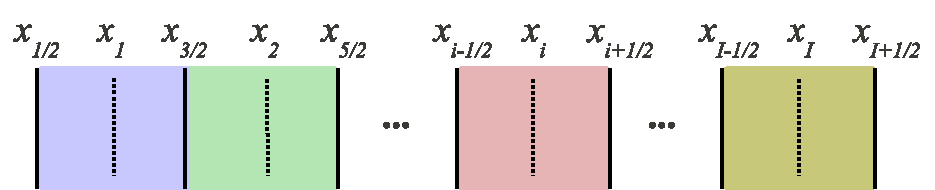
\includegraphics[keepaspectratio, width = 5.0 in]{images/sndisc}
    \caption{Discrete ordinates spatial discretization.}
    \label{fig:sndisc}
\end{figure}

Now, we integrate Eq. \ref{eq:snequation} over cell $i$:
\begin{equation}
  \int^{x_{i+\frac{1}{2}}}_{x_{i-\frac{1}{2}}} dx \Big ( \mu_n \frac{\partial \psi_n}{\partial x} + \Sigma_t(x)\psi_n(x) \Big ) =  \int^{x_{i+\frac{1}{2}}}_{x_{i-\frac{1}{2}}} dx  \Big ( \frac{\Sigma_s(x)}{2} \phi(x) + \frac{S(x)}{2} \Big ) \, ,
\end{equation}
so that
\begin{equation}
   \mu_n ( \psi_{i+\frac{1}{2},n} - \psi_{i-\frac{1}{2},n} ) + \Delta_i \Sigma_{ti}\psi_{i,n} =  \frac{\Delta_i}{2} \Big ( \Sigma_{is} \phi_i +  S_i \Big ) \, ,
\end{equation}
where $\Delta_i \equiv x_{i+\frac{1}{2}} - x_{i-\frac{1}{2}}$ and where the integrals have been approximated via the midpoint rule where needed.  For the sake of brevity, we switch to the emission density, defining
\begin{equation}
 Q_i =  (\Sigma_{is} \phi_i +  S_i)/2 \, ,
\end{equation}
so that
\begin{equation}
   \mu_n ( \psi_{i+\frac{1}{2},n} - \psi_{i-\frac{1}{2},n} ) + \Delta_i \Sigma_{ti}\psi_{i,n} =  \Delta_i Q_i \, .
   \label{eq:discsneq}
\end{equation}

Eq. \ref{eq:discsneq} is a good first step, but we're not done.  Imagine we know the angular flux entering the left side of slab $i$.  We would like to be able to compute the angular flux leaving $i$ to the right.  Doing exactly this over the entire domain is referred to as ``sweeping'' and is a common technique for hyperbolic problems, as it allows us to propagate boundary conditions along the direction of neutron paths.  The problem with Eq. \ref{eq:discsneq} is that we have another unknown: $\psi_{i,n}$, the cell-centered angular flux.  There are several approximations we can use, and we develop two: the diamond difference (DD) and step difference (SD) methods.

For both DD and SD, we define the cell-centered angular flux by
\begin{equation}
 \psi_{i,n} = \frac{1+\alpha_n}{2} \psi_{i+\frac{1}{2},n} + \frac{1-\alpha_n}{2} \psi_{i-\frac{1}{2},n}  \, ,
 \label{eq:ccpsi}
\end{equation}
where
\begin{equation}
 \alpha_n =
 \begin{cases} 0             &   \text{for DD}  \\
               |\mu_n|/\mu_n &   \text{for SD}  \\
 \end{cases} \, .
 \label{eq:alpha}
\end{equation}

The DD method is probably the most ubiquitous of the simple schemes available.  It essentially says the angular flux varies linearly within a cell, and it provides second-order accuracy.  Unfortunately, the DD method can lead to negative fluxes for $\Delta_i$ too large, demonstration of which is left as an exercise.  On the other hand, the SD method cannot yield negative fluxes, but is only first-order accurate.  For the SD method, note that the cell-center angular flux is equal to the incident angular flux at the edge.

\section*{Sweeping Formulas}

We hinted above that we can solve the discrete ordinates equations via use of sweeps across the domain.  In slab geometry, this consists of sweeps to the right for $\mu_n > 0$ and sweeps left for $\mu_n < 0$.  If we have vacuum or some other known boundary flux, we start with that condition, as reflective conditions require information from a sweep having come from the opposite direction.  If all conditions are reflective, a guess must be made for one, which will likely increase the number of iterations required (we'll get to iterations below).

Substituting Eq. \ref{eq:ccpsi} into Eq. \ref{eq:discsneq} and rearranging, we find for sweeping right
\begin{equation}
 \psi_{i+\frac{1}{2},n} = A^+_{i,n} \psi_{i-\frac{1}{2},n} + B^+_{i,n} Q_i \, ,
 \label{eq:rightsweep}
\end{equation}
and sweeping left
\begin{equation}
 \psi_{i-\frac{1}{2},n} = A^-_{i,n} \psi_{i+\frac{1}{2},n} + B^-_{i,n} Q_i \, , 
 \label{eq:leftsweep}
\end{equation}
where
\begin{equation}
 A^{\pm}_{i,n} = \frac{2\mu_n \mp (1 \mp \alpha_m)\Sigma_{ti}\Delta_i}{2\mu_n \pm (1 \pm \alpha_m)\Sigma_{ti}\Delta_i} \, , 
 \label{eq:Aconstant}
\end{equation}
and
\begin{equation}
 B^{\pm}_{i,n} = \frac{\pm 2 \Delta_i}{2\mu_n \pm (1 \pm \alpha_m)\Sigma_{ti}\Delta_i} \, .
 \label{eq:Bconstant}
\end{equation}

\section*{Source Iteration}

When we introduce scattering into the emission density, the right hand side becomes dependent on the solution.  A common way around this is the so-called source iteration method.  The source iteration method is related to the Neumann iteration scheme discussed in Lecture \ref{lec:integral}, and a connection between the two is left as an exercise.  

Source iteration is characterized by a right hand side that lags behind the left hand side.  More explicitly, we solve the equation
\begin{equation}
   \mu_n ( \psi^m_{i+\frac{1}{2},n} - \psi^m_{i-\frac{1}{2},n} ) + \Delta_i \Sigma_{ti}\psi^m_{i,n} =  \Delta_i Q^{m-1}_i \, ,
   \label{eq:discsneqsi}
\end{equation}
where $m$ is the iteration index and 
\begin{equation}
 Q^{m-1} = \frac{1}{2} (\Sigma_{is} \phi^{m-1}_i +  S_i) \, .
\end{equation}
For $m=1$, we need $q^0$.  Often, $\phi^0$ is simply set to zero, unless a better initial guess is easily made.  

The iterations continue until the updated fluxes change insignificantly.  This is usually quantified in a relative sense for the scalar flux by
\begin{equation}
 \frac{ \max | \phi^{m}-\phi^{m-1} |}{\phi^{m-1}}  < \epsilon_{\phi} \, 
 \label{eq:siconvergence}
\end{equation}
for some small $\epsilon_{\phi}$.

\section*{Acceleration}

The discrete ordinates method is in theory a very fast, memory-efficient technique.  Unless the angular flux is needed explicitly, only one set of edge angular fluxes is needed at a time (e.g. the left edge flux for computing the right edge flux, which then can overwrite the left edge flux).  

Despite the algorithmic simplicity of the method, the underlying source iteration scheme can be obnoxiously slow for problems with high scattering ratios.  Several methods have been introduced over the years to accelerate the source convergence.  Of these, diffusion synthetic acceleration (DSA) is probably the most powerful and widespread.  The method essentially involves performing a diffusion solve to update the scalar flux, and has shown spectacular success for a wide variety of problems.  However, DSA can be difficult if not impossible to implement for certain geometries and/or discretization schemes, as it requires a very strict consistency between the transport and diffusion mesh. Instead, we look at two other relatively simple methods that have been quite successful: the \textit{coarse mesh rebalance} (CMR) and \textit{coarse mesh finite difference} (CMFD) methods.

\section*{Coarse Mesh Rebalance}

CMR was probably the first wide-spread method for acceleration discrete ordinates calculations.  Its foundation rests in the \textit{neutron balance equation}, which we obtain in 1-d by integrating Eq. \ref{eq:slabtransportequation} over angle, yielding
\begin{equation}
\begin{split}
 \frac{\partial }{\partial x}J(x) + \Sigma_t(x) \phi(x) = \Sigma_{s}(x)\phi(x) + S(x) \, ,
\end{split}
\label{eq:balance}
\end{equation}
where $J = \mathbf{J}\cdot \hat{i}$ is the net current in the $x$ direction. Now suppose we divide the domain into a number of coarse meshes, indexed by $j$, with cell edges at $x_{j-\frac{1}{2}}$ and $x_{j+\frac{1}{2}}$.  Subtracting the scattering source from both sides and integrating over the $j$th coarse mesh, we obtain
\begin{equation}
\begin{split}
 J_{j+\frac{1}{2}} - J_{j-\frac{1}{2}}  + \int_{x_i} \Sigma_r(x) \phi(x) dx = \int_{x_i} S(x) dx \, .
\end{split}
\end{equation}
Expressing Eq. \ref{eq:net2partial} as $J = J^+ - J^-$, where $+$ indicates to the right and $-$ to the left, we have
\begin{equation}
\begin{split}
 J^+_{j+\frac{1}{2}}- J^-_{j+\frac{1}{2}} - J^+_{j-\frac{1}{2}} + J^-_{j-\frac{1}{2}} + R_j = S_j \, ,
\end{split}
\label{eq:cmrbalance}
\end{equation}
where the partial currents are defined
\begin{equation}
 J^{\pm}_{j+\frac{1}{2}} = \sum_{\mu_n \gtrless 0} \mu_n \psi_{j+\frac{1}{2},n} \, ,
\end{equation}
$R_j$ is the coarse mesh-integrated removal rate, and $S_j$ is the coarse mesh-integrated source.  

Eq. \ref{eq:cmrbalance} must be satisfied by a fully converged fine mesh solution.  For an unconverged iterate, which we denote $\psi^{m+\frac{1}{2}}$, Eq. \ref{eq:cmrbalance} is generally not satisfied.  To force the flux to satisfy neutron balance, we introduce multiplicative rebalance factors $f_j$ such that
\begin{equation}
 \psi^{m+1}_{i,n} =
 \begin{cases} f_j \psi^{m+\frac{1}{2}}_{i,n}     &   x_{j-\frac{1}{2}} < x_{i} < x_{j+\frac{1}{2}} \\
               f_{j-1} \psi^{m+\frac{1}{2}}_{i,n} &   x_{i} = x_{j+\frac{1}{2}} \text{ and } \mu_n > 0 \\
               f_{j+1} \psi^{m+\frac{1}{2}}_{i,n} &   x_{i} = x_{j+\frac{1}{2}} \text{ and } \mu_n < 0 \\
 \end{cases} \, .
 \label{eq:alpha}
\end{equation}
Note the appropriate factor's index denotes from which coarse mesh the neutrons originate. For the case of vacuum boundaries, the corresponding incident partial current vanishes.  For a reflective boundary at the left, $f_0 = f_1$, and similarly for the right boundary.

To illustrate the method, consider a slab with vacuum boundaries divided into three coarse meshes.  Substituting the modified fluxes into the balance equation yields a set of three equations:
\begin{equation}
\begin{split}
  f_1 J^+_{3/2}  - f_2 J^{-}_{3/2}                   + f_1 J^{-}_{1/2} + f_1 R_1 &= f_1 S_1 \\
  f_2 J^+_{5/2}  - f_3 J^{-}_{5/2} - f_1 J^{+}_{3/2} + f_2 J^{-}_{3/2} + f_2 R_2 &= f_2 S_2 \\
  f_3 J^+_{7/2}                    - f_2 J^{+}_{5/2} + f_3 J^{-}_{5/2} + f_3 R_3 &= f_3 S_3 \, ,
\end{split}
\end{equation}
which yields a tridiagonal system written in condensed form as
\begin{equation}
 \mathbf{A} \mathbf{f} = \mathbf{S} \, .
\end{equation}
Solving this equation for $\mathbf{f}$ and updating to $\psi^{m+1}$ allows us to recompute the scattering source, which---hopefully---converges faster than without the rebalancing scheme.  Look to the Further Reading section for references that investigate stability of coarse mesh rebalance.  Algorithm \ref{alg:accel} shows how CMR (or any low order acceleration scheme) can be used within source iteration.

\begin{algorithm}
 \label{alg:accel}
 \caption{Accelerated Source Iteration}
  initialization\;
  \While{$\psi^m$ or $\phi^m$ not converged}{
    compute scattering source \;
    $\psi^{m+\frac{1}{2}} \leftarrow \text{sweep}(\psi^{m})$ \;
    \eIf{using CMR}{
      $\psi^{m+1} \leftarrow \text{cmr}(\psi^{m+\frac{1}{2}})$ \;
    }{
      $\psi^{m+1} \leftarrow \psi^{m+\frac{1}{2}}$ \;
    }
  }
\end{algorithm}



\section*{Coarse Mesh Finite Difference}

The coarse mesh finite difference method has its origins in a nonlinear acceleration technique developed by K. Smith that makes use of discontinuity factors.  With discontinuity factors, any region-integrated high order solution (e.g. from fine mesh transport) can be represented by a low order method (e.g. coarse mesh diffusion).  CMFD makes use of this idea to represent partially converged high order solutions in low order form, followed by subsequent iterations in the low order domain.  This approach is a physical analog of multigrid methods, and its main effect is to dampen low order errors.  What this means is that the high order method will quickly get the ``shape'' right, and a low order acceleration will quickly get the ``magnitude'' right.

We sketch the implementation.  Given a partially converged fine mesh solution, homogenized diffusion coefficients and cross-sections are found for each coarse mesh, as are volume-averaged sources and fluxes.  A coarse mesh diffusion equation is to be solved, but due to an incompletely converged fine mesh solution, discontinuity factors---additive corrections to the effective diffusion coefficients---must be computed to enforce net current continuity between coarse meshes. Once these are defined, the coarse mesh diffusion equations can be solved.  The ratio of the updated average flux to the original average flux of a coarse mesh is used to scale the original fine mesh solution.  The interested student should see the references and exercises for further details.

%  For edge $j+\frac{1}{2}$ joining meshes $j$ and $j+1$, we compute from the high order solution the net current $J_{j+\frac{1}{2}}$ and enforce
% \begin{equation}
%  J_{j+\frac{1}{2}} = -\tilde{D}_{1+\frac{1}{2}} \Big ( \bar{\phi}_{j+1}-\bar{\phi}_{j} \Big ) -\hat{D}_{1+\frac{1}{2}} \Big ( \bar{\phi}_{j+1}-\bar{\phi}_{j} \Big ) \, ,
% \end{equation}
% where
% \begin{equation}
%  \D
% \end{equation}

\section*{A Simple Code}

Here, we provide a simple discrete ordinates code for computing the angular and scalar flux in a slab, given in Listing \ref{list:sn}.  The input requires region (coarse mesh) edge locations, within which the number of fine meshes are defined.  Each region is assigned a material index and volumetric source strength.  The total and scattering cross-sections represent values for different materials; each material can be placed in a region using the appropriate index.  This quick input format allows one to investigate fairly easily a wide range of slab compositions.

Currently, the code is limited to the DD and $S_4$ approximations and vacuum boundaries.  Convergence is tested for $\phi$ only.  The code returns the mesh-centered scalar flux and mesh-edge angular flux.  Within the solver, the notation follows the lecture notation relatively closely.

\lstset{language=Octave,caption=Solution of Slab Problem via Sn, label=list:sn, morecomment=[l]{\%}}
\lstinputlisting{code/sn.m}

% References
\section*{Further Reading}

A good introduction to the discrete ordinates method in 1-d can be found in Chapter 3 in Lewis and Miller \cite{lewis1993cmn}; higher dimensions are covered in Chapter 4 of the same work.  The foundation of the method is usually credited to Chandrasekhar (in the context of stellar radiation) and can be found in his monograph \cite{chandrasekhar1950rt}.  

A review paper by Adams and Larsen \cite{adams2002fim} provides a survey of the many acceleration techniques available for the discrete ordinates equations, and with its several hundred references, is the place to look for further information.  Lewis and Miller provides more information on coarse mesh rebalance, and Cefus and Larsen have assessed its stability \cite{cefus1990sac}.  Park and Cho \cite{park2004cma} have suggested angular-dependent rebalance schemes, and their work is a good place to start to find references to other CMR variations.  The discontinuity factors used in CMFD were first proposed by Smith in the context of homogenization \cite{smith1980shm}, and he later proposed their use for acceleration \cite{smith1983nms}. A recent paper by Zhong et al. \cite{zhong2008itl} provides a modern overview and advanced use of the approach along with a relatively detailed set of equations for implementation.  

Recent advances in the discrete ordinates method include employing advanced Krylov subspace methods, outlined by Warsa, Wareing, and Morel \cite{warsa2004kim}, variations of which are implemented in the state-of-the-art code Denovo \cite{evans2010dnt}.  Moreover, the discrete ordinates equations can be parallelized; the most popular approach is that of Koch, Baker, and Alcouffe \cite{koch1992sfo} (also implemented in Denovo).

For more information on numerical quadrature, see any number of numerical analysis books.  Also, MIT course 18.335 is also highly recommended, as it covers numerical quadrature and many other aspects of numerical methods (including a heavy focus on numerical linear algebra).

\begin{exercises}

  \item \textbf{Negative fluxes}. Using the DD method, express the sweeping step relation in the form
  \begin{equation*}
    \psi_{3/2,n} = A \psi_{1/2,n} + B \, ,
  \end{equation*}
  where $\mu_n > 0$ and $A$ and $B$ are constants to be determined, and eliminate any $\alpha$ terms.  Under what conditions can $\psi_{3/2,n}$ be negative?  Under what conditions, if any, can $\phi_{1,n}$ be negative?  While negative fluxes are not inherently bad numerically, they don't make much physical sense.  Suggest a method for ``fixing'' negative fluxes.

  \item \textbf{Step Difference}.  Implement the step difference method.\footnote{Note, in this and other exercises you are asked to use or modify the given $S_N$ code.  It is also acceptable to use your own code, either written from scratch or via modification of the one given.}

  \item \textbf{Step Characteristic}.  The step characteristic (SC) scheme is another differencing approach based on analytical integration of the transport equation over the fine mesh cell, yielding for example
  \begin{equation*}
    \psi_{i+\frac{1}{2},n}  =  \psi_{i-\frac{1}{2},n} e^{- \frac{\Delta_i \Sigma_{ti}}{\mu}} + \frac{Q_i}{2\Sigma_{ti}} \Big ( 1-e^{-\frac{\Delta_i \Sigma_{ti}}{\mu}} \Big ) \, .
  \end{equation*}
  \begin{enumerate}[(a)]
    \item Derive an expression for $\alpha_{mi}$ as in Eq. \ref{eq:alpha} for use with the SC method.  Note that $\alpha$ in this case is also indexed by the fine mesh index $i$. 
    \item Implement the SC method.
  \end{enumerate}
 
  \item \textbf{Accuracy}.  Here, we want to investigate the accuracy of various difference methods.  To do so, we will use a known analytical solution for as a reference.  See e.g. Appendix A of LeVeque \cite{leveque2007fdm} for more on error analysis.
  \begin{enumerate}[(a)]
    \item Using the $S_6$ approximation, solve \textit{analytically} the discrete ordinates equations for the sample slab problem of Lecture \ref{lec:analytical}.  Implement this reference solution as a function in MATLAB (or your language of choice), so that $\phi(x)$ can be evaluated for any value of $x$.        
    \item Using the DD approximation, solve the $S_6$ equations using 10, 20, 40, 80, and 160, and 320 meshes.  For each case, compute the absolute value of the maximum error between the DD and analytical solution for $\phi$, i.e. find 
    \begin{equation*}
     e^{\text{DD}}_I = \max_{1\leq i \leq I} \Big|\phi^{\text{DD}}_{i}-\phi_{i}^{\text{ref}} \Big |  \, .
    \end{equation*}
    \item Do the same for the SD method.
    \item We say a method is $p$th order accurate if $e(\Delta) \propto \Delta^p$.  Estimate $p$ for both methods. 
    \item Plot the errors for both methods as a function of $\Delta$.  Include also the functions $a\Delta^1$ and $b\Delta^2$, where $a$ and $b$ are constants chosen to yield a nice plot.  Hint: use a log-log plot.
   \end{enumerate}

  \item \textbf{Accuracy: Part Deux}.  Here, we want to investigate the accuracy of the Gauss-Legendre quadrature and hence $S_N$ order.  
  \begin{enumerate}[(a)]
    \item Compute $\phi(x)$ analytically for the sample slab problem of Lecture \ref{lec:analytical}, and make this available as a function.
    \item Compute $\phi$ analytically using the $S_N$ method for orders 2, 4, 8, 16, 32, and 64.  You will have to look up the quadrature parameters for $N > 4$.  
    \item Compute the errors in $\phi$ as in the last problem for $x = 5.0$ and plot as a function of $N$.  
    \item Estimate the ``$p$'' value as in the last problem and comment.  
   \end{enumerate}


  \item \textbf{Reflective Conditions}. Modify the given $S_N$ code to handle reflective conditions, and solve the following problems...

  \item \textbf{CMR}.  Implement CMR in the given $S_N$ code.  Test it on the following problems, using a variety of coarse mesh sizes...

  \item \textbf{CMFD}.  Read the paper by Zhong et al. \cite{zhong2008itl} and derive the CMFD equations in 1-d.  Implement the method in the $S_N$ code and compare it to CMR for the slab configuration given in the last problem.

  \item \textbf{Discrete Ordinates Matrix}.  The discrete ordinates equations are simply a set of coupled differential equations discretized in space and angle.  Consequently, we can express the equations in matrix form.  Consider a uniform slab ($\Sigma_t$ and $\Sigma_s$) with a uniform isotropic source of volumetric strength $S$. Suppose we discretize this slab into three cells of equal width $\Delta$.  Using an $S_2$ approximation with the DD method, and assuming vacuum conditions:
  \begin{enumerate}[(a)]
    \item Cast the sweep-based source iteration scheme in matrix form, expressing the right hand vector in terms of $Q$, the emission density.         
    \item Reformulate the equations so that the source term is brought to the left hand side, thus enabling a direct solution of the equations without source iteration.  
   \end{enumerate}
  For $\Sigma_t = 1.0$, $\Sigma_s = 0.5$, $\Delta = 1.0$, and $S = 1.0$, verify your expressions from parts (a) and (b).  For more on part (b), see the paper by Patton and Holloway \cite{patton2002apg}.

\end{exercises}

% 
\chapter{P$\mathrm{_N}$ Method and Diffusion}

\begin{exercises}

  \item  \textbf{P$_{\mathbf{1}}$ Boundary Conditions}. Derive the $P_1$ equations for isotropic scattering and an isotropic source.  Derive the Marshak vacuum conditions for arbitrary left and right boundaries in a slab.  Do the same for the Mark conditions. 

  \item \textbf{P$_{\mathbf{2}}$ Equations}.Show for the case of linearly anisotropic scattering and isotropic source that the $P_2$ equations can be written as a second order partial differential equation similar in form to the typical neutron diffusion equation.

  \item \textbf{Numerical Solution of the P$_{\mathbf{1}}$ Equations}. Consider a slab of width 10 cm with $\Sigma_t = 1.0$ [cm$^{-1}$], and $c = \Sigma_s / \Sigma_t = 0.5$ (isotropic scattering in the lab system).  A uniform, isotropic source of $1$ [n/cm$^2$-s] is located in the first half of the slab, and both slab edges are subject to vacuum conditions. Write a code to solve the $P_1$ approximation to this problem using Marshak conditions.  Plot $\psi(x,\mu)$ at $x = 0$, $2.5$, $5.0$, $7.5$, and $10$ [cm].  Plot $\phi(x)$ over the whole slab.

  \item \textbf{Numerical Solution of the P$_{\mathbf{3}}$ Equations}. For the same problem, write a code to solve the $P_3$ approximation using Marshak conditions.

  \item \textbf{ Diffusion via asymptotics}.  Consider the following rescaling of the 1-d, mono-energetic transport equation with isotropic scattering. Finish me.

  \item \textbf{Legendre Addition Theorem}. Prove the Legendre polynomial addition theorem.  You may use any resource you want, but make sure you understand all steps of the proof.  A particularly straightforward approach begins as follows.  Start with an expansion of an arbitrary function in the full spherical harmonics.  Then, substitute the definition of the expansion coefficients back into the expansion.  Noting that the integral and summation can be switched, what function must the summation be?  

  \item \textbf{Defining the Scattering Angle}. Prove $\mu_0 = \cos(\theta)\cos(\theta')+\sin(\theta)\sin(\theta')\cos(\phi-\phi')$, where $\mu_0$ is the cosine of the scattering angle and ($\theta$,$\phi$) and $(\theta',\phi')$ are the original and final angles, respectively.  Include a diagram.

\end{exercises}

% \chapter[Linearity and Reciprocity]{Linearity of the Transport Equation and Reciprocity Relations}
\label{lec:linearity}
% \chapter{The Adjoint and Perturbation Theory}
\label{lec:adjoint}

In this lecture, we introduce the \textit{ adjoint} form of the transport equation and describe what it represents physically.  We then apply the adjoint equation in a useful technique known as \textit{first order} or \textit{linear perturbation theory}.  In the next lecture, we make further use of the adjoint in the context of variational approximations.

\section*{The Adjoint Function}

We define the \textit{ inner product} of two  functions $\phi(x)$ and $\psi(x)$ to be
\begin{equation}
  \langle \phi, \psi \rangle \equiv \int \phi(x) \psi(x) dx \, ,
\end{equation}
where $\phi$ and $\psi$ satisfy appropriate continuity and boundary conditions.  A \textit{self-adjoint} operator $M$ satisfies
\begin{equation}
  \langle \phi, M \psi \rangle \equiv  \langle M \phi, \psi \rangle  \, .
\end{equation}
As an example, the operator corresponding to one-speed diffusion can be shown to be self-adjoint, an exercise left to the reader.  Note, self-adjoint and \textit{hermitian} are synonymous.  You may be familiar with the latter term from quantum physics, and you might recall that such operators (say the Hamiltonian) have real eigenvalues (like the energy) and orthogonal eigenfunctions (such as the nice sines and cosines of the infinite well).

If an operator $L$ is not self-adjoint, it is possible to define an operator $L^*$ that is adjoint to $L$.  Then $L^*$ will operate on adjoint functions $\psi^*(x)$ that may satisfy different boundary conditions than those of $\psi(x)$ on which $L$ operates.  The adjoint operator $L^*$ must satisfy
\begin{equation}
  \langle \psi^*, L \psi \rangle =  \langle \psi, L^* \psi^* \rangle  \, ,
  \label{eq:adjointidentity}
\end{equation}
which we refer to as the \textit{adjoint identity} (and which is actually a special case of a generalized Green's theorem).

\section*{Transport Operator}
We now define the transport equation in operator form.  Defining the operator 
\begin{equation}
  \begin{split}
     L\psi & \equiv -\hat{\Omega} \cdot \nabla \psi(\mathbf{r},\mathbf{\Omega},E) \\
           & -\Sigma_t \psi + \int^{\infty}_{0} dE' \int_{4\pi} d\Omega' \Sigma_s(\mathbf{r},\mathbf{\Omega}\cdot\mathbf{\Omega}',E'\to E)\psi(\mathbf{r},\mathbf{\Omega'},E') \, ,
  \end{split}
  \label{eq:transportoperator}
\end{equation}
the transport equation is simply $L \psi = -Q$, for some source $Q$; note the sign of the right hand side.  The transport operator $L$ is \textit{not self-adjoint}.  Convince yourself that this is indeed the case by evaluating the adjoint identity and paying specific attention to the terms corresponding to streaming and scattering.  For convenience, we assume $\psi$ is also subject to vacuum conditions on all external surfaces, i.e. $\psi(\mathbf{r},\mathbf{\Omega},E)=0$ for $\hat{n}\cdot \hat{\Omega} < 0$ where $\hat{n}$ is the outward normal vector.

The adjoint transport operator $L^*$ will satisify $\langle \psi^*, L \psi \rangle =  \langle \psi, L^* \psi^* \rangle $, if and only if we define it such that
\begin{equation}
  \begin{split}
     L^*\psi^* & \equiv \hat{\Omega} \cdot \nabla \psi^*(\mathbf{r},\mathbf{\Omega},E) \\
               & -\Sigma_t \psi^* + \int^{\infty}_{0} dE' \int_{4\pi} d\Omega' \Sigma_s(\mathbf{r},\mathbf{\Omega}\cdot\mathbf{\Omega}',E\to E')\psi^*(\mathbf{r},\mathbf{\Omega'},E') \, ,
   \end{split}
   \label{eq:adjointoperator}
\end{equation}
with the further restriction that $\psi^*(\mathbf{r},\mathbf{\Omega},E)=0$ for $\hat{n}\cdot \hat{\Omega} > 0$. It's worth noting we could have chosen conditions other than vacuum boundaries for $\psi$, which would yield different conditions for $\psi^*$; see the exercises for the case of reflecting boundaries.

\section*{Interpreting the Adjoint}

Let's consider a subcritical, time-independent system containing an arbitrary source.  Suppose we are interested in a detector response with an associated cross-section $\Sigma_d(\mathbf{r},E)$.  Then we have the forward equation
\begin{equation}
  \begin{split}
     &\hat{\Omega} \cdot \nabla \psi(\mathbf{r},\mathbf{\Omega},E) + \Sigma_t \psi = \\
     &\int^{\infty}_{0} dE' \int_{4\pi} d\Omega' \Sigma_s(\mathbf{r},\mathbf{\Omega}\cdot\mathbf{\Omega}',E'\to E)\psi(\mathbf{r},\mathbf{\Omega'},E') + Q(\mathbf{r},\mathbf{\Omega},E)  \, ,
  \end{split}
  \label{eq:foreq}
\end{equation}
subject to vacuum conditions, and the adjoint equation
\begin{equation}
  \begin{split}
     -&\hat{\Omega} \cdot \nabla \psi^*(\mathbf{r},\mathbf{\Omega},E) + \Sigma_t \psi^* = \\
     &\int^{\infty}_{0} dE' \int_{4\pi} d\Omega' \Sigma_s(\mathbf{r},\mathbf{\Omega}\cdot\mathbf{\Omega}',E\to E')\psi^*(\mathbf{r},\mathbf{\Omega'},E')  \, ,
  \end{split}
  \label{eq:adjeq}
\end{equation}
subject to the appropriate conditions.  Here, the detector cross-section, which can be thought of as a ``detector response function'', is the adjoint source.  Now, we multiply Eq. \ref{eq:foreq} by $\psi^*$ and Eq. \ref{eq:adjeq} by $\psi$, subtract the latter from the former, and integrate over all variables to get (operator and inner-product notation)
\begin{equation}
 \langle \psi^*, L \psi \rangle - \langle \psi, L^* \psi^* \rangle = - \langle \psi^*, Q \rangle +  \langle \psi, \Sigma_d \rangle \, ,
\end{equation}
but by the adjoint identity, the left hand side vanishes, and we are left with a most important result:
\begin{equation}
 \langle \psi^*, Q \rangle =  \langle \psi, \Sigma_d \rangle \, .
 \label{eq:adjrule}
\end{equation}
Suppose our forward source is a unit monoenergetic, unidirectional point source, i.e. $Q(\mathbf{r},\mathbf{\Omega},E) = \delta(\mathbf{r}-\mathbf{r}_0)\delta(\mathbf{\Omega}-\mathbf{\Omega}_0)\delta(E-E_0)$.  From Eq. \ref{eq:adjrule}, we find
\begin{equation}
 \psi^*(\mathbf{r}_0,\mathbf{\Omega}_0,E_0) = \int_V d^3r \int_{E} dE \int_{4\pi} d\Omega \Sigma_d(\mathbf{r},E') \psi(\mathbf{r},\mathbf{\Omega},E) = R \, ,
\end{equation}
where $R$ is the total detector response.  In this case, $\psi^*(\mathbf{r}_0,\mathbf{\Omega}_0,E_0)$ is the expected contribution to the detector response due to a unit delta source located at $(\mathbf{r}_0,\mathbf{\Omega}_0,E_0)$ in phase space.  More broadly, $\psi^*$ represents the importance of neutrons in a particular region of phase space to a given detector response.

\section*{Perturbation Theory --- Fixed Source}

In this and the next section, we apply the adjoint in determining the change to an integral system parameter\footnote{Here, an ``integral'' parameter is any integrated quantity, e.g. a reaction rate in a volume, or $k_{e\!f\!f}$ in a reactor.} due to a small perturbation in the system.  We begin with a fixed source example and follow with an eigenvalue example.

Suppose we have a system described by\footnote{Note, the operators in this section have absorbed the minus sign of the right hand side sources above.}
\begin{equation}
 L_0 \psi_0 = Q_0 \, 
\end{equation}
with vacuum boundaries.  Our goal is to evaluate a detector response that takes the form
\begin{equation}
 R_0 = \int \int \int d^3r d\Omega dE \Sigma_d(\mathbf{r},E) Q(\mathbf{r},E,\mathbf{\Omega}) \, .
\end{equation}

Suppose we now introduce some small change.  Perturbation theory can allow us to determine the detector response, to first order accuracy, for a ``small'' perturbation to the system.  Let us define a new, perturbed system to be
\begin{equation}
 L \psi = Q \, ,
\end{equation}
also subject to vacuum conditions, and where $L = L_0 + \delta L_0$, $Q = Q_0 + \delta Q_0$, and $\psi = \psi_0 + \delta \psi_0$.  We assume we know $L$ and $Q$ (we're making the perturbation), and we want to know $\psi$ (and eventually, its effect on $R$). Rewriting the system, we have
\begin{equation}
\begin{split}
 ( L_0 + \delta L_0)(\psi_0 + \delta \psi_0) &= Q_0 + \delta Q_0 \\
  L_0 \psi_0 + \delta L_0 \psi_0 + L_0 \delta \psi_0 + \theta(\delta^2) &= Q_0 + \delta Q_0 \, ,
\end{split}
\end{equation}
but noting our original equation is contained, we are left with two separate equations,
\begin{equation}
 L_0 \psi_0 = Q_0 \, ,
 \label{eq:pertzeroth}
\end{equation}
and
\begin{equation}
 \delta L_0 \psi_0 + L_0 \delta \psi_0 = \delta Q_0 \, ,
 \label{eq:pertfirst}
\end{equation}
where we have neglected terms of order $\delta^2$; hence the theory is known as ``first order'' or ``linear'' perturbation theory.

We now introduce the adjoint to the \textit{original equation}, with the adjoint source being our detector response function $\Sigma_d$, i.e.
\begin{equation}
 L^*_0 \psi^*_0 = \Sigma_d \, ,
 \label{eq:pertadj}
\end{equation}
and as before, we have $\langle \psi^*_0, Q_0 \rangle =  \langle \psi_0, \Sigma_d \rangle = R_0$.  Our goal is to determine $\delta R_0$, or $R-R_0 = \delta R_0 =  \langle \delta \psi_0, \Sigma_d \rangle$.  To do so, we multiply Eq. \ref{eq:pertfirst} by $\psi^*_0$ and Eq. \ref{eq:pertadj} by $\delta \psi_0$, subtract the latter from the former, and integrate over all phase space, yielding
\begin{equation}
  \langle \psi^*_0, \delta L_0 \psi_0 \rangle + \langle \psi^*_0, L_0 \delta \psi_0 \rangle - \langle L^*_0 \psi^*_0, \delta \psi_0 \rangle = \langle \psi^*_0, \delta Q_0 \rangle - \langle \delta \psi_0, \Sigma_d \rangle \, .
\end{equation}
The second and third terms on the left hand side cancel by way of the adjoint identity, and the second term on the right hand side is $\delta R_0$.  Thus, we have
\begin{equation}
 \delta R_0 = \langle \psi^*_0, \delta Q_0 \rangle - \langle \psi^*_0, \delta L_0 \psi_0 \rangle \, .
 \label{eq:fixedpertresp}
\end{equation}
From Eq. \ref{eq:fixedpertresp}, we see that an increased source gives rise to a \textit{greater} response, and an increase in $L$, corresponding to greater leakage or interaction, produces a \textit{lower} response, as is expected.

\section*{Perturbation Theory --- Eigenvalue}

As another example of perturbation theory, consider the unperturbed eigenvalue problem
\begin{equation}
 H_0 \psi_0 = \lambda_0 F_0 \psi_0 \, 
\end{equation}
subject to vacuum conditions.  As above, suppose we introduce some small change, and let a new, perturbed system be
\begin{equation}
  H \psi = \lambda F \psi \, .
\end{equation}
where $H = H_0 + \delta H_0$, $F = F_0 + \delta F_0$, $\psi = \psi_0 + \delta \psi_0$, and $\lambda =\lambda_0 + \delta \lambda_0$.  Our goal is to find $\delta \lambda_0$ due to the perturbation.  

We rewrite the perturbed system
\begin{equation}
 (H_0 + \delta H_0)(\psi_0 + \delta \psi_0) = (\lambda_0 + \delta \lambda_0)(F_0 + \delta F_0)(\psi_0 + \delta \psi_0) 
\end{equation}
and expand
\begin{equation}
\begin{split}
  H_0 \psi_0 + \delta H_0 \psi_0 &+ H_0 \delta \psi_0 + \theta(\delta^2) \\
      &= \lambda_0 F_0 \psi_0 + \lambda_0 F_0 \delta \psi_0 + \lambda_0 \delta F_0 \psi_0 + \delta \lambda_0 F_0 \psi_0 + \theta(\delta^2)  \, .
\end{split}
\end{equation}
Again, we recognize our original equation and a second equation with first-order perturbations,
\begin{equation}
 (H_0 - \lambda_0 F_0) \delta \psi_0 = (\lambda_0 \delta F_0 \psi_0 ) - (\delta H_0 - \delta \lambda_0 F_0)\psi_0 \, .
 \label{eq:eigenpertfirst}
\end{equation}

We define the adjoint problem
\begin{equation}
 H^*_0 \psi^*_0 = \lambda_0 F^*_0 \psi^*_0 \, 
 \label{eq:eigenpertadj}
\end{equation}
subject to the appropriate boundary conditions.  Similar to our treatment in the fixed source example, we multiply Eq. \ref{eq:eigenpertfirst} by $\psi^*_0$ and Eq. \ref{eq:eigenpertadj} by $\delta \psi_0$, subtract the latter from the former, and integrate over all phase space.  After a bit of rearranging, we find
\begin{equation}
 \delta \lambda_0 = \frac{\langle \psi^*_0,(\delta H_0 - \lambda_0 \delta F_0)\psi_0 \rangle}{\langle \psi^*_0, F_0 \psi_0 \rangle} \, .
 \label{eq:eigenpertresp}
\end{equation}

\section*{Further Reading}

Most of the development here follows that of Bell and Glasstone \cite{bell1970nrt}, Chapter 6.  Duderstadt and Hamilton \cite{duderstadt1976nra} develop the adjoint within the diffusion framework and apply it to problems of reactor physics in Chapters 5 and 7.  A particularly appealing description of the physical interpretation of the adjoint, albeit with a reactor physics flavor, is given by Henry \cite{henry1975nra}.  

It's worth noting that the adjoint was developed first by Lagrange as a mathematical construct; however, its physical utility was first realized much later in the context of quantum mechanical perturbation theory, and later yet in reactor physics.  This history and more is to be found in Marchuk's treatise on adjoint methods \cite{marchuk1995aea}.  That first application of the adjoint in reactor physics was due to the ``father of nuclear engineering,'' Eugene Wigner \cite{wigner1945esp}.  

The available literature on perturbation theory is quite large.  One important recent effort has been to couple sensitivities defined by perturbation theory to cross-section uncertainties in order to estimate the uncertainty of integral system parameters including the eigenvalue \cite{broadhead2004sau} and various worths \cite{williams2007sau} due to the underlying data uncertainty.  

\begin{exercises}

  \item \textbf{Self-adjointness}. Prove the one-speed diffusion operator, i.e. $L\phi = D\phi_{xx} - \Sigma_a\phi(x) = -S$ is self-adjoint.  You may assume a homogeneous medium with zero-flux boundary conditions, neglecting extrapolation distances.

  \item \textbf{Adjoint Transport Equation}. Demonstrate that the adjoint operator $L^*$ defined by Eq. \ref{eq:adjointoperator} really is the adjoint to the forward operator $L$ for the given boundary conditions.

  \item \textbf{Adjoint Boundary Conditions}. (a) For the case that $\psi$ satisfies vacuum conditions, we found that $\psi^*(\mathbf{r},\mathbf{\Omega},E)=0$ for $\hat{n}\cdot \hat{\Omega} > 0$.  What does this mean physically?  (b) For the one-speed transport equation, derive the boundary conditions for $\psi^*$ when $\psi$ satisfies reflecting conditions.

  \item \textbf{Using the Adjoint}. (a) Briefly describe the physical meaning of the adjoint flux. (b) Suppose we have a known shield with a known detector on one side.  Suppose further that the particle source on the opposite side of the shield is not known \textit{a priori} and can take widely varying forms.  (An example of this might be a shielding analysis for a fusion reactor, where we think we have a good shield and then we try using it for several possible sources).  How could the adjoint be used so that only one ``transport'' calculation would be needed to compute the detector dose given an arbitrary source?

  \item \textbf{A Point Detector}. Repeat the process used to obtain $\psi^* = R$ but for the case of a point detector, $\Sigma_d = \delta(\mathbf{r}-\mathbf{r}_0)\delta(\mathbf{\Omega}-\mathbf{\Omega}_0)\delta(E-E_0)$.  Clearly, one obtains an expression for $\psi(\mathbf{r}_0,\mathbf{\Omega}_0,E_0)$.  What does $\psi^*(\mathbf{r},\mathbf{\Omega},E)$ represent in this case?  This result is a generalization of reciprocity relations previously discussed for one-speed transport.

  \item \textbf{The ``Contributon'' Flux}. In 1-d and one-speed, define the quantity 
  \begin{equation*}
   C(x,\mu) = \psi(x,\mu)\psi^*(x,\mu) \, ,
  \end{equation*}
  where $\psi$ and $\psi^*$ are the forward and adjoint angular fluxes.  Take the forward problem to have vacuum boundaries.  (a) Mathematically, express the vacuum boundary condition for $\psi$ at a general external boundary $x_b$.  (b) With your knowledge of the corresponding adjoint boundary condition, write down the mathematical expression for the boundary condition of $C(x,\mu)$.  (c) Taking the adjoint source to be a flux-to-dose factor, what are the units of $\psi$, $\psi^*$, and $C$?  Can you interpret $C$ physically?  (For more information on this mysterious quantity, see the paper by Williams \cite{williams1991gcr}.)

  \item \textbf{Eigenvalue Perturbation}.  Prove Eq. \ref{eq:eigenpertresp}.  Also, describe what possible changes in the system coincide with the perturbations $\delta H_0$ and $\delta F_0$ and how such changes impact the eigenvalue perturbation.  Remember that $k_{e\!f\!f}$ is $\lambda^{-1}$.

  \item \textbf{Eigenvalue Sensitivity}.  Defining the sensitivity of $k_{e\!f\!f}$ to a cross-section $\Sigma_x$ to be
  \begin{equation*}
   S_{k,\Sigma_x} = \frac{\Sigma_x}{k_{e\!f\!f} }\frac{\partial k_{e\!f\!f}}{ \partial \Sigma_x} \, ,
  \end{equation*}
  find an expression for $S_{k,\Sigma_x}$ in terms of the partial derivatives of $H_0$ and $F_0$ with respect to $\Sigma_x$.


\end{exercises}

% \chapter{Variational Methods}

In this lecture, we investigate use of \textit{variational principles} in the 
context of nuclear engineering.  An entire course could be devoted to this 
subject; here, we focus on the same two quantities analyzed in 
Lecture \ref{lec:adjoint}, namely the reaction rate for a fixed source problem 
and the eigenvalue of an eigenvalue problem.  We demonstrate that variational 
principles can be used to estimate these quantities using approximate fluxes. 
We finish by showing how our first order perturbation theory can be derived 
directly from variational principles.

%------------------------------------------------------------------------------%
\section*{Variational Principles, Functionals, and Stationary Points}

A variational principle casts a particular function, usually a problem's 
solution, as the stationary point of some \textit{functional}. Often, the 
functional itself is called the variational principle.  A functional is 
simply a function that takes another function as its argument and returns 
a scalar as its value.  Consider a function $f(x) = Ax + B$.  A possible 
functional would be $F[f(x)] = \int_{x_1}^{x_2} f(x)dx$, which certainly 
yields a scalar value.  Typically, the value of the functional represents 
a quantity of interest, which in transport applications is often a 
reaction rate.

We see that functionals are quite like functions; how exactly then do we 
define a \textit{stationary point}, and what does it mean in the context 
of a variational principle?  Recall from elementary calculus that a stationary 
point is the value of the independent variables such that the function reaches 
a local extremum (or saddle-point), i.e. the function's derivative (or 
gradient) vanishes.  The same idea applies to functionals.  Defining 
the ``weak derivative'' of $F$ at a point $f(x)$ in the direction $g(x)$ as
\begin{equation}
 \delta F[f,g] = \lim_{\epsilon \to 0} 
                 \frac{ F[f+\epsilon g] - F[f] }{\epsilon} \, ,
\end{equation}
the \textit{first variation} of $F$ is defined 
\begin{equation}
 \delta F[f,g] = \left ( \frac{d}{d\epsilon} F[f+\epsilon g] \right ) 
                 \Bigg |_{\epsilon = 0} \, ,
\end{equation}
for arbitrary $g$.  When $\delta F[\tilde{f},g] = 0$ for all $g$, $\tilde{f}$ 
is called a \textit{stationary point} of $F$, and the expression
\begin{equation}
 \delta F[\tilde{f},g] = 0 \, ,  \, \, \, \, \, \, \forall g 
\end{equation}
defines the variational principle for $\tilde{f}$.  For $F[f]$ that represents 
a quantity of interest, $F[\tilde{f}]$ represents the true value for that 
quantity.  Moreover, very near the stationary point, $\delta F \to 0$ by 
construction, and the errors in $F$ (and hence the quantity of interest) are 
second order, which gives rise to the utility of variational approximations.

%------------------------------------------------------------------------------%
\section*{A Simple, Illustrative Example}

It is easiest to understand these ideas through a simple example (unrelated 
to nuclear engineering).  Suppose we wish to find the curve giving us the 
shortest difference between two points in a plane  Of course, this is 
intuitive: the solution should be a line.  We show this using variational 
techniques.  

Let the curve be $f(x)$. From any calculus book, we know the differential arc 
length is then
\begin{equation}
 dl = \sqrt{ dx^2 + df^2 } = \sqrt{1 + (f')^2} \, .
\end{equation}
We take as our functional the arc length,
\begin{equation}
 F[f] = \int^{x_2}_{x_1} \sqrt{1 + (f')^2} dx \, ,
\end{equation}
where ($x_1$, $y_1$) and ($x_2$, $y_2$) are the points of interest, as 
illustrated in Figure \ref{fig:shortest_path}.

\begin{figure}[ht] 
    \centering
    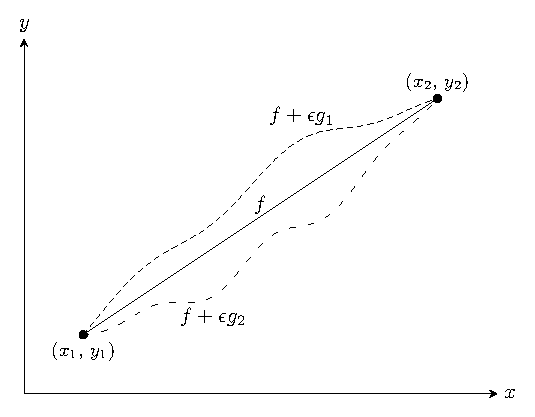
\includegraphics[keepaspectratio, width = 4.0 in]{images/shortest_path}
    \caption{The shortest path between two points ($x_1$, $y_1$) and 
            ($x_2$, $y_2$) is indicated by the solid curve $f$.  Two possible
            curves for arbitrary $g$ are also given.}
    \label{fig:shortest_path}
\end{figure} 

Taking the first variation of $F$,
\begin{equation}
\begin{split}
\delta F[f,g] &= \left ( \frac{d}{d\epsilon}\int^{x_2}_{x_1} 
                         \sqrt{1 + (f'(x)+\epsilon g'(x))^2} dx \right ) 
                 \Bigg |_{\epsilon=0} \\
              &= \left ( \int^{x_2}_{x_1} 
                         \frac{(f'(x)+\epsilon g'(x))g'(x)}
                              {\sqrt{1 + (f'(x)+\epsilon g'(x))^2}} \right ) 
                 \Bigg |_{\epsilon=0} \\
              &= \int^{x_2}_{x_1} \frac{f'(x)g'(x)dx}{\sqrt{1 + (f'(x))^2}} \, ,
\end{split}
\end{equation}
we find that the arc length is minimized when
\begin{equation}
 \delta F[y,g] =
   \int^{x_2}_{x_1}\frac{f'(x)g'(x)}{\sqrt{1 + (f'(x))^2}} = 0 \, .
 \label{eq:exampleprinciple}
\end{equation}
In this form, we can't say anything about $f$ or $g$.  Instead, we use 
integration by parts to go from $f'$ and $g'$ to $f''$ and $g$, and
Eq. \ref{eq:exampleprinciple} becomes
\begin{equation}
 \delta F[f,g] =
   \left [ \frac{f'(x)g(x)}{\sqrt{1 + (f'(x))^2}} \right ]^{x_2}_{x_1} - 
   \int^{x_2}_{x_1} \frac{f''(x)g(x)dx}{(1 + (f'(x))^2)^{\frac{3}{2}}} = 0\, .
 \label{eq:exampleprinciple2}
\end{equation}
While $g(x)$ is arbitrary \textit{between} $x_1$ and $x_2$, we must have 
$g(x_1) = g(x_2) = 0$ to that $f(x_1) = y_1$ and $f(x_2) = y_2$.  Thus, the 
first term of Eq. \ref{eq:exampleprinciple2} vanishes. 
By inspection, the second term vanishes for 
arbitrary $g$ only if $f'' = 0$.  This relation is known as 
the \textit{Euler equation}\footnote{In general, setting the first variation 
to zero gives rise to a set of partial differential equations collectively 
known as the Euler equations.}.  Of course, to satisfy $f''=0$ requires 
our solution to be of the form $Ax+B$, as expected.

%------------------------------------------------------------------------------%
\section*{A Variational Principle for Fixed Source Problems}

Suppose we are interested in a linear functional of the flux, such 
as $G_{\text{fs}}[\psi] = \langle \psi, \Sigma_d \rangle$, a reaction rate. 
An appropriate variational principle is represented by 
the \textit{generalized Roussopoulos functional}
\begin{equation}
 F_{\text{fs}} [\psi,\psi^*] = 
   G_{\text{fs}}[\psi] + \langle \psi^*, (Q-L\psi) \rangle \, .
\end{equation}
Note, $\delta F_{\text{fs}}[\psi,\psi^*] = 0$ is a variational principle 
for $G_{\text{fs}}$ if the corresponding solution $\psi$ 
yields $F_{\text{fs}}[\psi,\psi^*] = G_{\text{fs}}[\psi]$.  We see this is 
so when the second term of $F$ vanishes when $\psi$ solves $L\psi = Q$, i.e. 
when $\psi$ is the solution to the transport equation.

To determine the variational principle, we take the first variation 
of $F_{\text{fs}}$,
\begin{equation}
 \begin{split}
  \delta F_{\text{fs}} & [\phi,\phi^*] \\
   &= \left ( \frac{d}{d\epsilon} 
            \left ( \langle (\phi+\epsilon \delta \phi) \Sigma_d \rangle + 
                    \langle (\phi^* + \epsilon \delta \phi^*), 
                            (Q-L(\phi+\epsilon \delta \phi)) \rangle 
            \right ) 
    \right ) \Bigg|_{\epsilon=0} \\
   &= \langle \delta \phi, \Sigma_d \rangle - 
      \langle \phi^*,L \delta \phi \rangle + 
      \langle \delta \phi^*, Q \rangle - 
      \langle \delta \phi^*, L \phi \rangle +
      \mathcal{O}(\epsilon^2) \, .
 \end{split}
\end{equation}
Noting 
$\langle \phi^*,L\delta \phi \rangle = \langle L^* \phi^*,\delta \phi \rangle$, 
we have for our principle 
\begin{equation}
 0 = \langle \delta \phi, (\Sigma_d - L^* \phi^*) \rangle + 
     \langle \delta \phi^*, (Q-L\phi) \rangle \, ,
\end{equation}
which is satisfied when $L\phi = Q$ and $L^* \phi^* = \Sigma_d$.  These are 
the corresponding Euler equations, and we see they are just the original 
forward and adjoint transport equations.

The importance of this variational principle (and others in general) is that 
it gives us an estimate for $G_{\text{fs}}$ accurate to second order for 
approximate fluxes $\phi$ and $\phi^*$.  To demonstrate this, suppose the 
true solutions to the Euler equations are $\psi$ and $\psi^*$.  
Let $\phi = \psi + \delta \psi$ and $\phi^* = \psi^* + \delta \psi^*$.  
We subsitute these expressions into $F$ and find
\begin{equation}
 \begin{split}
    F_{\text{fs}} [\phi,\phi^*] &= 
      \langle \Sigma_d, (\psi+\delta \psi) \rangle + 
      \langle (\psi^*+\delta \psi^*),(Q-L(\psi+\delta \psi^*) \rangle \\
    &= \langle \Sigma_d,\psi \rangle + 
       \langle \Sigma_d, \delta \psi \rangle + 
       \langle \psi^*,Q \rangle + 
       \langle \delta \psi,Q \rangle  \\ 
    &- \langle \psi^*, L\psi \rangle - 
       \langle \psi^*, L\delta \psi \rangle - 
       \langle \delta \psi^*, L\psi \rangle - 
       \langle \delta \psi^*, L\delta \psi \rangle \\
    &= \langle \Sigma_d, \psi \rangle - 
       \langle \delta \psi^*, L\delta \psi \rangle \\
    &= G_{\text{fs}}[\psi] + \mathcal{O}(\delta^2) \, .
 \end{split}
 \label{eq:secondorderfs}
\end{equation}
Hence, $F$ provides a first order accurate (i.e. good through first order) 
estimate of the reaction rate given approximate forward and adjoint fluxes.

\section*{A Variational Principle for Eigenvalue Problems}

For eigenvalue problems, an appropriate functional is 
the \textit{Rayleigh quotient}
\begin{equation}
 F_{\text{ev}}[\psi,\psi^*] = 
   \frac{\langle \psi^*,L\psi \rangle}{ \langle \psi^*, F \psi \rangle } \, .
 \label{eq:rayleigh}
\end{equation}
Here, the quantity of interest is $G_{\text{ev}} = \lambda$, and, unlike the 
fixed source case, we have $G_{\text{ev}} = F_{\text{ev}}$.  You should show 
that $F_{\text{ev}}$ is in fact a valid expression for $\lambda$.  The 
associated Euler equations are just the forward and adjoint eigenvalue 
equations, which can be shown by setting the first variation 
of $F_{\text{ev}}$ to zero, an exercise left to the reader.
For approximate fluxes $\phi$ and $\phi$
\begin{equation}
 F_{\text{ev}}[\phi,\phi^*] = \lambda + \mathcal{O}(\delta^2) \, ,
\end{equation}
the proof of which is also left as an exercise.

\section*{Perturbation Theory from Variational Principles}

In general, it is possible to find first order perturbation estimates using 
the expression
\begin{equation}
 \delta = \bar{F}[\psi,\psi^*] - F[\psi,\psi^*] \, ,
 \label{eq:pertfromvar}
\end{equation}
where $F$ is the appropriate functional with nominal operators 
and $\bar{F}$ is the function evaluated with perturbed operators.  It must 
be stressed that $\psi$ and $\psi^*$ are assumed to be the exact fluxes for 
the unperturbed problem.

As an example, we re-derive the first order perturbation to a detector 
response.  Suppose the perturbations to our system 
include $L+\delta L$, $Q+\delta Q$, 
and $\Sigma_d + \delta \Sigma_d$.  Then Eq. \ref{eq:pertfromvar}  gives
\begin{equation}
\begin{split}
 \delta_{\text{fs}} &= \bar{F}[\psi,\psi^*] - F[\psi,\psi^*] \\
        &= \langle \psi, (\Sigma_d+\delta \Sigma_d) \rangle + 
           \langle \psi^*,(Q+\delta Q-(L+\delta L)\psi ) \rangle - 
           \langle \psi, \delta \Sigma_d \rangle \\
        &= \langle \psi,\delta \Sigma_d \rangle + 
           \langle \psi^* , \delta Q \rangle - 
           \langle \psi^*,\delta L \psi \rangle \, .
\end{split}
\label{eq:fixedpertvar}
\end{equation}
The last line is equivalent to Eq. \ref{eq:fixedpertresp} with the addition 
of the first term, which explicitly accounts for changes in the detector 
response function.

Eq. \ref{eq:pertfromvar} can also be applied to the Rayleigh quotient, 
yielding Eq. \ref{eq:eigenpertresp}, proof of which is left 
as an exercise.

%------------------------------------------------------------------------------%
\section*{Further Reading}

Most of the material presented here is contained in Chapter 7 of 
Duderstadt and Martin \cite{duderstadt1976tt}  in addition to Chapter 1 
of Stacey \cite{stacey1974vmn}.  The former contains several examples 
and a variational derivation of the diffusion equation.  The reader is 
also encouraged to look up Pomraning's large body of work on variational 
methods\footnote{It is worth noting that Stacey and Pomraning, both with 
prolific work in variational methods, did their graduate work in 
this department.}.

%------------------------------------------------------------------------------%
\begin{exercises}

  %----------------------------------------------------------------------------%
  \item \textbf{Second Order Accuracy}. 
    Show that the Roussopoulos functional $F[\phi,\phi^*]$ gives a second 
    order accurate value for $\langle \psi,\Sigma_d \rangle$ when $\phi$ 
    and $\phi^*$ are approximate values of $\psi$ and $\psi^*$, i.e. 
    prove Eq. \ref{eq:secondorderfs}.

  %----------------------------------------------------------------------------%
  \item \textbf{Fixed Source Perturbation}. 
    Prove Eq. \ref{eq:fixedpertvar}.
 
  %----------------------------------------------------------------------------%
  \item \textbf{Rayleigh Quotient}. 
    \begin{enumerate}[a.]
      \item Take the first variation of the Rayleigh quotient with respect to 
            the forward and adjoint fluxes and show the stationarity conditions 
            are just the forward and adjoint eigenvalue problems. 
      \item Demonstrate that the Rayleigh quotient is a second order 
            estimator for $\lambda$.
    \end{enumerate}

  %----------------------------------------------------------------------------%
  \item \textbf{Losses-to-Gains}. 
    Directly from the eigenvalue equation, we find 
    \begin{equation*}
      \lambda = (L\psi)/(F\psi) \, ,
    \end{equation*}
    a compact way to define losses-to-gains.  
    \begin{enumerate}[a.]
      \item Show why this is not a variational principle for $\lambda$.
      \item Consider again Eq. \ref{eq:rayleigh}.  How does the adjoint change 
            the physical interpretation of gains-to-losses?
    \end{enumerate}

  %----------------------------------------------------------------------------%
  \item  \textbf{Eigenvalue Perturbation}. 
    Prove that $\bar{F}_R[\psi,\psi^+]-F_R[\psi,\psi^+]$ yields the first 
    order perturbation estimate for $\delta \lambda$ given 
    by Eq. \ref{eq:eigenpertresp}.

  %----------------------------------------------------------------------------%
  \item  \textbf{Applying Roussopoulos}. 
    Consider a 1-d, 1-speed diffusion problem in a slab of 
    width $2a$, $\Sigma_a = 0.022$, and $D = 0.14$. 
    \begin{enumerate}[a.]
      \item Solve for the exact scalar flux $\phi(x)$, using the 
            conditions $\phi(\pm a)=0$, and
            assuming a uniform source $Q(x) = 1$ and $a=1$.
      \item Compute the total absorption rate in the slab.
      \item Now, approximate the solution as 
            $\tilde{\phi}(x) = Ax^2 + Bx +C$ with the same maximum 
            and the same boundary conditions.  Compute the absorption rate  
            using $\tilde{\phi}(x)$.
      \item Finally, recalling the 1-d, 1-speed diffusion equation is 
            self-adjoint, use the Roussopoulos principle to compute the 
            absorption rate.  What can you conclude? 
    \end{enumerate}

  %----------------------------------------------------------------------------%
  \item \textbf{More Roussopoulos}. 
    For the same problem, estimate the total absorption rate if something 
    causes $\Sigma_a = 1.1$.  Be careful to consider the impact of the change 
    in $\Sigma_a$ on both $\Sigma_d$ and $L$.

  %----------------------------------------------------------------------------%
  \item \textbf{Approximating Escape from a Slab}. 
    Recall the escape probability $P_{\text{esc}}$ for a homogeneous 1-d slab, 
    the subject of 
    Chapter \ref{lec:analytical}, Problem \ref{itm:escapeprobability}.  
    Here, consider a discrete ordinates approximation using the 
    two point Gauss-Legendre quadrature and Mark boundary conditions
    for a 10 cm slab with $\Sigma_t = 10$ [1/cm].
    \begin{enumerate}[a.]
      \item Solve for $P_{\text{esc}}$ directly using the S$_{\text{2}}$ 
            approximation.
      \item Use a variational principle to improve 
            your estimate of $P_{\text{esc}}$. 
      \item Compare both values to the exact value.
    \end{enumerate}

\end{exercises}

% 
% 
% \part{Bibliography and Appendices} 
% 
% % Reset to a simple chapter title and format
% \renewcommand\printchaptertitle[1]{%
%     \begin{tabular}{@{\Large\bfseries\chaptername}@{ }p{1.0cm}!{\quad}p{\textwidth-4cm-2em-4\tabcolsep }}
%       \ifNoChapNumber\relax\else\chapnumfont \thechapter\fi
%       & \chaptitlefont 
%     \end{tabular}
%     \NoChapNumberfalse
% }
% \renewcommand{\chaptername}{Bibliography}
% \bibliographystyle{plain}
% \bibliography{biblio106}
% 
% 
% \appendix
% \renewcommand{\chaptername}{Appendix}
% \chapter{Nomenclature}

To facilitate understanding of the various terms used throughout the lecture materials, we provide here a list of variables, short definitions, and common units where applicable.  In very few cases, symbols are used more than once due to convention (e.g. $\phi$ for both flux and azimuthal angle).  Bold symbols indicate a vector quantity.

\begin{table}[th]
 \caption{Fundamental quantities}
 \begin{center} 
 {\small
 \begin{tabular*}{0.90\textwidth}{@{\extracolsep{\fill}} ccc } 
  \toprule 
   Symbol                            & Description   & Units  \\
  \midrule 
   $\psi(\vec{r},\hat{\Omega},E,t)$          & angular flux                  & $\frac{\mathrm{n}}{\mathrm{cm^2-s-eV-ster}}$  \\
   $\psi^+(\vec{r},\hat{\Omega},E,t)$        & adjoint angular flux          & $\frac{\mathrm{n}}{\mathrm{cm^2-s-eV-ster}}$  \\
   $\phi(\vec{r},E,t)$                       & scalar  flux                  & $\frac{\mathrm{n}}{\mathrm{cm^2-s-eV}}$  \\
   $\phi^+(\vec{r},E,t)$                     & adjoint scalar flux           & $\frac{\mathrm{n}}{\mathrm{cm^2-s-eV}}$  \\
   $\mathbf{j}(\vec{r},\hat{\Omega},E,t)$    & angular current density       & $\frac{\mathrm{n}}{\mathrm{cm^2-s-eV-ster}}$  \\
   $\mathbf{ J}(\vec{r},E,t) $               & current density               & $\frac{\mathrm{n}}{\mathrm{cm^2-s-eV}}$  \\
   $J_{\pm}(\vec{r},E,t)$                    & partial current density       & $\frac{\mathrm{n}}{\mathrm{cm^2-s-eV}}$  \\
  \bottomrule 
 \end{tabular*} 
 }
 \end{center} 
 \label{tbl:snmeshstudy}  
\end{table}


% %
\chapter{Numerical Solution of the Diffusion Equation}
\label{app:diffusion}

We covered the $P_N$ equations and how the diffusion equation is formally derived in Lecture \ref{pn_method_and_diffusion}.  In this lecture, we revisit the diffusion equation for slab geometry and develop a straightforward differencing scheme for its numerical solution.  We provide a simple code that performs multigroup diffusion for fixed source and eigenvalue (reactor) problems.

\section*{The Diffusion Equation}

\section*{Albedo Conditions}

\section*{Difference Schemes}

\section*{Further Reading}



\begin{exercises}

  \item \textbf{Boundary Sources}.  Modify the albedo condition given in Eq. ?? to include a boundary source. 

  \item \textbf{Diffusion in 2-d}.  Derive the difference equations for diffusion in 2-d Cartesian geometry following the procedure used for 1-d above.

\end{exercises}


\end{document}